%--------|---------|---------|---------|---------|---------|---------|---------|
%       10        20        30        40        50        60        70        80
%-------------------------------------------------------------------------------


% Make sure you have a good editor. This file is _way_ too large to be really practical to work with. I should split it up into at least a few sections, e.g: campaign, side quests, appendices, playthrough. But since I'm writing this mainly on a small laptop, on the go, with an excellent text editor, it's actually faster for me to keep it in one single file. I'm lacking the multiple monitor screen space I'm used to. Love my 3x portrait 24" 4k workspace!
% If you're going to do any significant work in here please contact me and I'll split it all up.





\documentclass[11pt, twoside, titlepage, a4paper]{article}
% set utf8 encoding, and set font encoding T1 to allow "|" ">" "<" etc
\usepackage[utf8]{inputenc}
\usepackage[T1]{fontenc}
\usepackage[a4paper,inner=40mm,outer=25mm,top=25mm,bottom=25mm,pdftex]{geometry}
% These page settings give images 1.0\linewidth around 135-140mm wide (ca 138mm)
% meaning a 300dpi image is around 1600 pixels wide
\usepackage{graphicx}   % For eps figures
\usepackage{epsfig}     % Alternative package
\usepackage[hang,small,bf]{caption}

\usepackage[british]{babel}       

\usepackage[yyyymmdd]{datetime}
\renewcommand{\dateseparator}{--}

\usepackage{fancyhdr}
\pagestyle{fancy}
% with this we ensure that the chapter and section
% headings are in lowercase.
%\renewcommand{\chaptermark}[1]{\markboth{#1}{}}  % no "\chapter" in article doc type
\renewcommand{\sectionmark}[1]{\markright{\thesection\ #1}}
\fancyhf{} % delete current setting for header and footer
\fancyhead[LE,RO]{\bfseries\thepage}
\fancyhead[LO]{\bfseries\rightmark}
\fancyhead[RE]{\bfseries\leftmark}
\renewcommand{\headrulewidth}{0.5pt}
\renewcommand{\footrulewidth}{0pt}
\addtolength{\headheight}{0.5pt} % make space for the rule
\fancypagestyle{plain}{%
    \fancyhead{} % get rid of headers on plain pages
    \renewcommand{\headrulewidth}{0pt} % and the line
}


% remove forced implicit vertical whitespace before and after verbatim environment
\makeatletter
\preto{\@verbatim}{\topsep=0pt \partopsep=0pt }
\makeatother


% allow to force indentation of first line in section
% \indent is not working, so workaround \hspace{\parindent} works
\newcommand{\forceindent}{\hspace{\parindent}}


\newcommand{\degrees}{$^\circ$~}
\newcommand{\degree}{$^\circ$}
\newcommand{\ca}{$\approx$}

\newcommand{\vs}{$\backslash\ $}  % "versus" slash
\newcommand{\bs}{$\backslash\ $}  % just backslash


% want clear dash insert commands
\newcommand{\dash}{-}     % just a normal hyphen dash  "-"
\newcommand{\ndash}{--}   % n-dash "--"
\newcommand{\mdash}{---}  % m-dash "---"


%link new command names to the original font sizes,
%for easier to remember smaller font size
\newcommand{\vsmall}{\footnotesize}  % simpler to remember
\newcommand{\vvsmall}{\scriptsize}   %
%\newcommand{\vvvsmall}{\tiny}


\usepackage[colorlinks=true,linkcolor=black,urlcolor=blue]{hyperref}


\usepackage{ifthen}


% \needspace{5\baselineskip}      << reserves approximately 5 lines, leaves raggedbottom, more efficient
% \Needspace{5\baselineskip}      << reserves exactly 5 lines, leaves raggedbottom, less efficient
% \Needpsace*{5\baselineskip}     << leaves flushbottom if \flushbottom is in effect, otherwise ragged
\usepackage{needspace}



% \skill{blabla}
\newboolean{skillsaslist}
\setboolean{skillsaslist}{true}
\ifthenelse{\boolean{skillsaslist}}{\newcommand{\skill}[1]{\item[#1]}}{\newcommand{\skill}[1]{\subsubsection*{#1}}}
\ifthenelse{\boolean{skillsaslist}}{\newcommand{\openskillslist}{\begin{description}}}{\newcommand{\openskillslist}{}}
\ifthenelse{\boolean{skillsaslist}}{\newcommand{\closeskillslist}{\end{description}}}{\newcommand{\closeskillslist}{}}

% \action{blabla}
\newboolean{actionsaslist}
\setboolean{actionsaslist}{true}
\ifthenelse{\boolean{actionsaslist}}{\newcommand{\action}[1]{\item[#1]}}{\newcommand{\action}[1]{\subsubsection*{#1}}}
\ifthenelse{\boolean{actionsaslist}}{\newcommand{\openactionslist}{\begin{description}}}{\newcommand{\openactionslist}{}}
\ifthenelse{\boolean{actionsaslist}}{\newcommand{\closeactionslist}{\end{description}}}{\newcommand{\closeactionslist}{}}

% \eqitem{blabla}
\newboolean{itemsaslist}
\setboolean{itemsaslist}{true}
\ifthenelse{\boolean{itemsaslist}}{\newcommand{\eqitem}[1]{\item[#1]}}{\newcommand{\eqitem}[1]{\subsubsection*{#1}}}
\ifthenelse{\boolean{itemsaslist}}{\newcommand{\openitemslist}{\begin{description}}}{\newcommand{\openactionslist}{}}
\ifthenelse{\boolean{itemsaslist}}{\newcommand{\closeitemslist}{\end{description}}}{\newcommand{\closeactionslist}{}}


\newenvironment{readoutloud}%
{\begin{quote}\begin{itshape}}%
{\end{itshape}\end{quote}}%



% need a nice easily visible TODO marker
\newcommand{\todo}{\textbf{TODO:}~}
\newcommand{\TODO}{\LARGE\textbf{TODO:}\normalsize~}







%-------------------------------------------------------------------------------
\begin{document}



% DONE: set hyphenation language to UK English  >>  see settings.article above
% Manually specify hyphenation for names, etc. 
% Remember: space separated word list: lead with space.
% hyphens can only occur on specified "-" characters, 
% words without hyphens will never be hyphenated, overrides language rules
% see link regarding location of hyphenation block
% https://en.wikibooks.org/wiki/LaTeX/Text_Formatting#Hyphenation
\hyphenation{ 
 Gammel-Tant 
 Gam-ling 
 Hemske-lina 
 Go-blan-da 
 Stur-Skurk 
 Hjal-mar Hjäl-te 
 Bur-mak 
 Lund-qvist 
 Grim-Gnash 
 Evil-nius 
 Thing-a-ma-jig 
 Gros-Orc 
 muta-mon-ster 
 muta-meat 
 Iffy-Griff 
 Hoo-man Hoo-mans hoo-man hoo-mans 
 Da-tar-i-an Ma-ras No-stro-mo 
}





%-------------------------------------------------------------------------------
% make a simple title page
%-------------------------

%-------------------------------------------------------------------------------
% cover page for work in progress, remove when completed
%-------------------------------------------------------

\thispagestyle{empty}

\null          % make an empty mark, so that following white space will be honoured
\vspace{4cm}   % not honoured at beginning of page without something above

\begin{center}

\huge
Goblin Destiny

\vspace{0.3\baselineskip}

\large
Death by GrimGnash

\vspace{2cm}

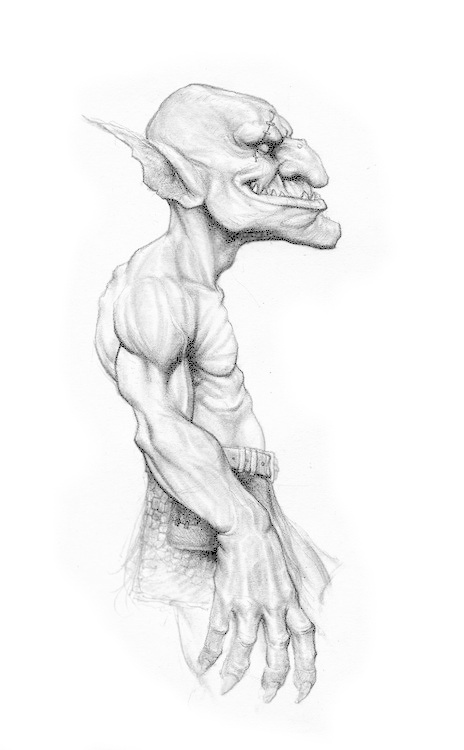
\includegraphics[width=50mm]{./fig/goblinside.jpg}

\vspace{2cm}

\normalsize
finished campaign\\
cleanup in progress\\

\vfill

\today

\end{center}






%-------------------------------------------------------------------------------
% copyright etc on the back side of the title page
%-------------------------------------------------
\clearpage
\thispagestyle{empty}
\raggedbottom

\vsmall
\noindent 
This work is licensed under a Creative Commons \\
Attribution-NonCommercial-ShareAlike 4.0 \\
International License. (CC BY-NC-SA 4.0).\\
\url{https://creativecommons.org/licenses/by-nc-sa/4.0/} \\
\url{https://creativecommons.org/licenses/by-nc-sa/4.0/legalcode} \\
If you want to use it in any other fashion please contact the author.

\

\noindent
All images are temporary placeholders, \\
most are downloaded and unattributed.\\
They need to be replaced with licensed art.

\normalsize






%-------------------------------------------------------------------------------
% begin main matter
%------------------
\cleardoublepage
\pagestyle{fancy}
\flushbottom

%\setcounter{page}{1}


% will mark both left and right pages with an abbreviated section title
% since this is most likely to be read on screens one page at a time instead of
% printed in a binder/book with left/right pages visible simultaneously.
%\markboth{lefttitle}{righttitle}


%\mainmatter  -- nope, not in article




%--------|---------|---------|---------|---------|---------|---------|---------|
%       10        20        30        40        50        60        70        80
%-------------------------------------------------------------------------------
\section*{Goblin Destiny}
\markboth{goblin destiny}{goblin destiny}

A silly campaign, playing Villainous Goblins fighting to survive against long odds.

\

\noindent \textbf{These misadventures} follow the GamGang goblin clan and their struggle to carve out a tiny slice of the world for themselves. Their land and livelihood is invaded by another group of bandits and their Fearless Leader Gamling dies during a highway robbery. The old prophecy of \emph{Death by GrimGnash} is coming true...

\

\tableofcontents                                   % sets page header "CONTENT"
\markboth{goblin destiny}{goblin destiny}          % restore the page headers

\vspace{4\baselineskip}

% ensure enough space left on page (15 lines), or flush a new \clearpage
% so as not to break the introduction too early
\needspace{15\baselineskip}

\phantomsection\addcontentsline{toc}{section}{introduction}
\subsection*{Introduction}

The campaign should be more fun than serious. Crazy adventures, plans gone wrong, comical stupidity and short-sightedness. The fights are challenging. Goblins have issues with planning, discipline, and lower hp and strength than most typical heroes.

Early on the Heroes will improve their situation, gaining loot and experience. As their banditry grows so does the response from the law and order in the region. Patrols are more frequent. Loot is more difficult to sell. Specialised troops start hunting them. Occasionally they will find long lost dungeons, plan revenge assaults, go on monster hunts and shopping sprees, scouting for real estate, and other non-bandit activities. In the end most Heroes will die or flee when they finally face GrimGnash. Regardless, the GamGang clan is no more after GrimGnash is done.

%\todo include ?
%Perhaps even Burmak or Lundqvist manage to root out enough of the gang to close the campaign, but it's more fun if you can balance it on the thin edge so it's difficult, two steps forward, one step back, survival by flight to fight another day.

\

\noindent \textit{Goblin life ain't easy!}

\

\


\subsection*{Campaign outline}

The following adventures make up the main campaign arc. They are intended as milestones. Inject the other small adventures between them.

\begin{description}

    \item[another day in the office] A short intro fight to get the players oriented with their characters. Just some farmers, guards, and a bit of loot.

    \item[robbery gone wrong] Another band of robbers show up during a routine highway robbery. Gamling dies. GammelTant is the new Leader and calls for Revenge! She recognises the first sign of the Dread Prophecy of \emph{Death by GrimGnash}.

    \item[kill the bandits] The murderous invaders must be killed. Their camp has been scouted. An attack in the middle of the night is the brilliant idea to revenge Gamling and kill off the competition.

    \item[defend Hoom Hool] The Horrible Hoomans have banded together and hired some adventurers to root out the goblin clan. The Heroes must defend their Hoom Hool cave.

    \item[flee and relocate] The Horrible Hoomans try again and again, eventually they succeed. Forcing the goblins to flee and find somewhere else to nest.

    \item[GrimGnash] They go to certain death when they to kill GrimGnash to escape the \emph{Death by GrimGnash} prophecy. Perhaps a few characters flee and survive for future adventures, perhaps they all die.

\end{description}

\


\noindent Below are small intermission adventures that are not part of the main campaign arc and can usually be played at any time. Insert the ones that tickles your fancy,  where suitable.

\begin{description}

    \item[patrols] When travelling the gang runs into patrols. Discuss, bluff, bribe, or fight. The patrolmen are not automatically confrontational. If the gang can pass for traders, travellers, or other civilians they can even get some information, or an escort on their way. Later on the patrols will be hunting for them specifically.

    \item[iffygriff eggs] They have spotted IffyGriffs flying to an area in The Moors. An old outpost has an IffyGriff nest, a small warband, and a haunted guard tower with a cursed sword.

    \item[mutamonsters] A magical place in the forest which turns goblins and critters into strange monsters. They can fight their way to the magic source and get strange mutated abilities and magic-ified equipment.

    \item[torture dungeon] They have found a treasure map pointing to somewhere in the Duns. Ruins of a tower with an old torture dungeon below filled with undead, black bugs, a strange trap, and some loot.
    
    \item[mountain hools] Central BlackPeak mountains hold a few caves. Occupied of course, but perhaps suitable for the relocating clan after aggressive negotiations.

    \item[plunder] Perhaps a few road side ambushes or village periphery raids to gather some coin? Or food, or just some stuff to trade for food?

    \item[fishy burglary] They have heard that a Richy Rich is staying in the tavern \emph{Sleeping with the Fishes}. Must be worth sneaking in and plunder his room and stuff.

    \item[shopping] At some point they might want to go shopping for food or gear, or to sell some loot. Who knows what can be found in a nearby village? Some soldiers perhaps?

\end{description}

\noindent The Heroes can also go on other adventures, extra raids, weekend shopping sprees, etc. As long as they have enough food to feed GamGang they are more or less free to do what they want. But when GammelTant's stomach starts growling it's dangerous to be around the cook pot empty handed ...


\subsection*{The GamGang clan}

Gamling leads the Gang with an iron fist and an empty head. GammelTant is smarter but will not be leading until after Gamling dies.
At the start of the campaign the GamGang crowd is about 30 heads strong. Approximately 20 goblins, including the Heroes, and some 10+ runts, wolves, critters, etc.

The whole gang, including heroes, require lots of food each day. Food scarcity, lack of money, lack of good loot, etc, should be common and urgent for most, if not all, of the campaign. Gamling and GammelTant will get angry when the food runs low, and in the end start cooking the goblins or runts they dislike the most, including uppity obnoxious Heroes.

Generally, life in the bandit gang is simple. You help find food and loot. Steal, hunt, gather, or whatnot. You avoid ending up in the cook pot. And you keep doing this ... until you don't.


\subsection*{Goblin Destiny~\mdash~\emph{Death by GrimGnash}}   %\,\textendash\,

The prophecy says that when The Great Leader dies by The Blue Boss, GamGang must kill GrimGnash or be themselves destroyed.

GrimGnash is a dragon and there is no way the Goblins will win that fight. Thus, the destiny of the goblins is to die! \emph{Mostly}. Some might escape and appear in later campaigns.


\subsection*{What's with Goblins?}

Playing a goblin band is a bit different from a regular group of adventurers. Goblins are lazy, cowardly, blood thirsty, often hungry, live day to day and are poor planners.

Finding enough food should be an issue, pushing the Heroes to never sit still for long. They will be tasked with feeding the whole gang, and even though Gamling has money in the coffer he won't give any to the Heroes to buy food. A slain human is a delicacy and can feed the whole gang for a day. Try to have smart enemies flee when things turn sour. Less loot, money, and food. 

Remember that goblins don't speak Common by default. Don't remind them. If none of the Heroes bothered to learn Common they won't be able to communicate with most humans. And if they have low Common skill let them roll for the communication and be merciless with injecting misunderstandings and misinterpretations. Hilarious. 
% see mail 180115

% https://tex.stackexchange.com/questions/7627/how-to-reference-paragraph
\phantomsection \label{misunderstandings}
Some goblins even have very low Svartlingo skills. They can't understand or communicate complex sentences or unusual topics easily, even when talking amongst the gang. Have the players use only simple words, pidgin grammar, short sentences, and so on.

\begin{quote}
\begin{small}

On their way to Sleepy Cove, two wagons with eight brave goblins roll north over the grassland. Dawn, barely an hour after they've crawled out of their potato sack sleeping bags, eaten some cold snails, and gotten under way. In the distance a small group of humans approach. A man on horse and three more walking, relaxed. Closing slowly they carry spears and shields, uniformed. The man on horse rides ahead a little bit and and waves to the goblins as he approaches from a distance.

\begin{description}

\item[Fizzleflare:] \vvsmall (svartlingo) \small
"He waves his men to reinforce, mussst kill'im qvick!"

\item[Patrolman rider:] \vvsmall (common, shouts from distance) \small 
"Hi, hi. Hello over there!"

\item[GamGang:] \vvsmall (svartlingo, giggling amongst themselves) \small 
"Slaughter smashing! Hehe!"

\item[Heidiblast:]
"I'll prepare a black bolt! Will blow his head clean off!"

\end{description}
... the patrol squad approaches casually ...
\begin{description}

\item[Patrolman rider:] \vvsmall (common) \small
"Hi there Happy Tradesmen, how's the beautiful morning treating you? What lovely sunshine we have! And to think that Sanna the Seer claimed it would rain. Haha."

\item[Old Maz:] \vvsmall (fail common, broken svartlingo) \small
"What 'im say?"

\item[Kizraz:] \vvsmall (fail common, broken svartlingo) \small
"Clue no have. No-Know."

\item[Grapplebottom:] \vvsmall (fail common, broken svartlingo) \small
"What understand? Speak Talk?"

\end{description}
... and so on until Fizzleflare manages to understand ...
\begin{description}

\item[Fizzleflare:] \vvsmall (broken common) \small
"We come southfrom. Fishesh. Go Sleepy Cove."

\item[Patrolman rider:] \vvsmall (common) \small
"Ah. How nice! Please be careful when travelling the area south of town. There is a band of horrible goblin bandits in the woods. Hjalmar Hjälte is in Sleepy Cove gathering a posse to go deal with them. He think they live out of the old goblin warren which Datarian, Maras, and Nostromo cleaned out before the Big Demon Rampage. But why are you coming this strange way? The road is much faster."

\item[Old Maz:] \vvsmall (fail common, broken svartlingo) \small
"What say he?"

\item[Kizraz:] \vvsmall (fail common, broken svartlingo) \small
"No understand gabbadigook!"

\item[Fizzleflare:] \vvsmall (broken common) \small
"Öööh-hum. Big Bandit! Attacked! SturSkurk! Blue Sword. Orcsesh and Fishesh."

\item[Patrolman rider:] \vvsmall (common) \small
"Another bandit? Oh no! We don't have enough patrols out on the roads these days. Not since the Demon Rampage killed off Baron Pawa. SturSkurk? With Blue Swords and fishing orcs? Apologies, I don't quite understand?"

\end{description}
Meanwhile, the Röbank brothers walk up to the rider and looks at his horse.
\begin{description}

\item[Dunkab Röbank:] \vvsmall (fail common: "Hey! Give us horse or we beat the blood out of you:") \small
== "Hurru! Hours-yet grave ooze! Moor ley banshee blood lay Flanders!"

\item[Patrolman rider:] \vvsmall (common) \small
"Uhm? Excuse me. I didn't quite understand. Could you please repeat that?"

\end{description}

And here Smashesh Röbank has lost his patience and bashes the horse in the head with his large club. So the murdering begins!

After a surprisingly quick fight the goblins have a wounded horse and four human cadavers to feast on. They promptly forget about trading in Sleepy Cove and instead turn back to Hoom Hool to celebrate.

\end{small}
\end{quote}


\subsection*{Practicalities}

Goblins are squishy but numerous. The players run two goblins each. This is fun and different but an impractical design on my part. Play testing with up to six players controlling two Heroes each, plus sidekicks, meant very large and thus slow fights for part of the campaign. To keep the speed up consider using simplified rules or have the players control only one goblin each and scale down the opposition accordingly. \emph{But}, some of the fights are spectacular when the players have a small army of crazy goblins to throw around. The main playthrough was done with 8-20 Heroes and sidekicks zerging around on the board at all times.

As the Heroes die off roll replacement goblins with (85+1D10)\% of the the xp of the dead one. The first two goblin Heroes the player starts the campaign with should come from a rolled set of five, then each replacement from a new set of three. Use \verb|rollchars.py| to quickly roll sets of goblins.

For players that absolutely don't want to play goblins, have them play a single Hero from another race. Choose a race and roll a small set of characters from that race only (human 2, dwarf 1, elf 1, halfling 2, orc 1). Any elf here should probably have a mental disability to live in a goblin gang, or perhaps they are anthropologists studying the life of the native lesser races?

It can be fun to allow all the goblins to have the effect of infinite prescient training. I.e: they can spend xp to learn skills at any time, not just in between sessions or adventures. This makes for a lot of comedy situations. E.g: \emph{Oh Sh*t! I'm about to die! I'll buy possum to 8.}


\subsection*{This corner of the world ...}

GamGang is new to the region. They have fled from unknown southlands after being chased out by orcs. On their way north they found two battered goblins. The two used to belong to a bandit gang who had a great hool in the bountiful forest south of Sleepy Cove. Then some Heroes came and slaughtered most of them a while back, a crazy bloodthirsty armoured dwarf and some others. After Gamling promises them a place in GamGang they tell him all about their Hoom Hool, Bestest LootSpot, Skaary plains, Hoomans, etc. GammelTant then promptly wrings their necks and cooks them. The gang was short on food, as usual, and goblins are decent eating.

\begin{figure}[h!]
  \centering
  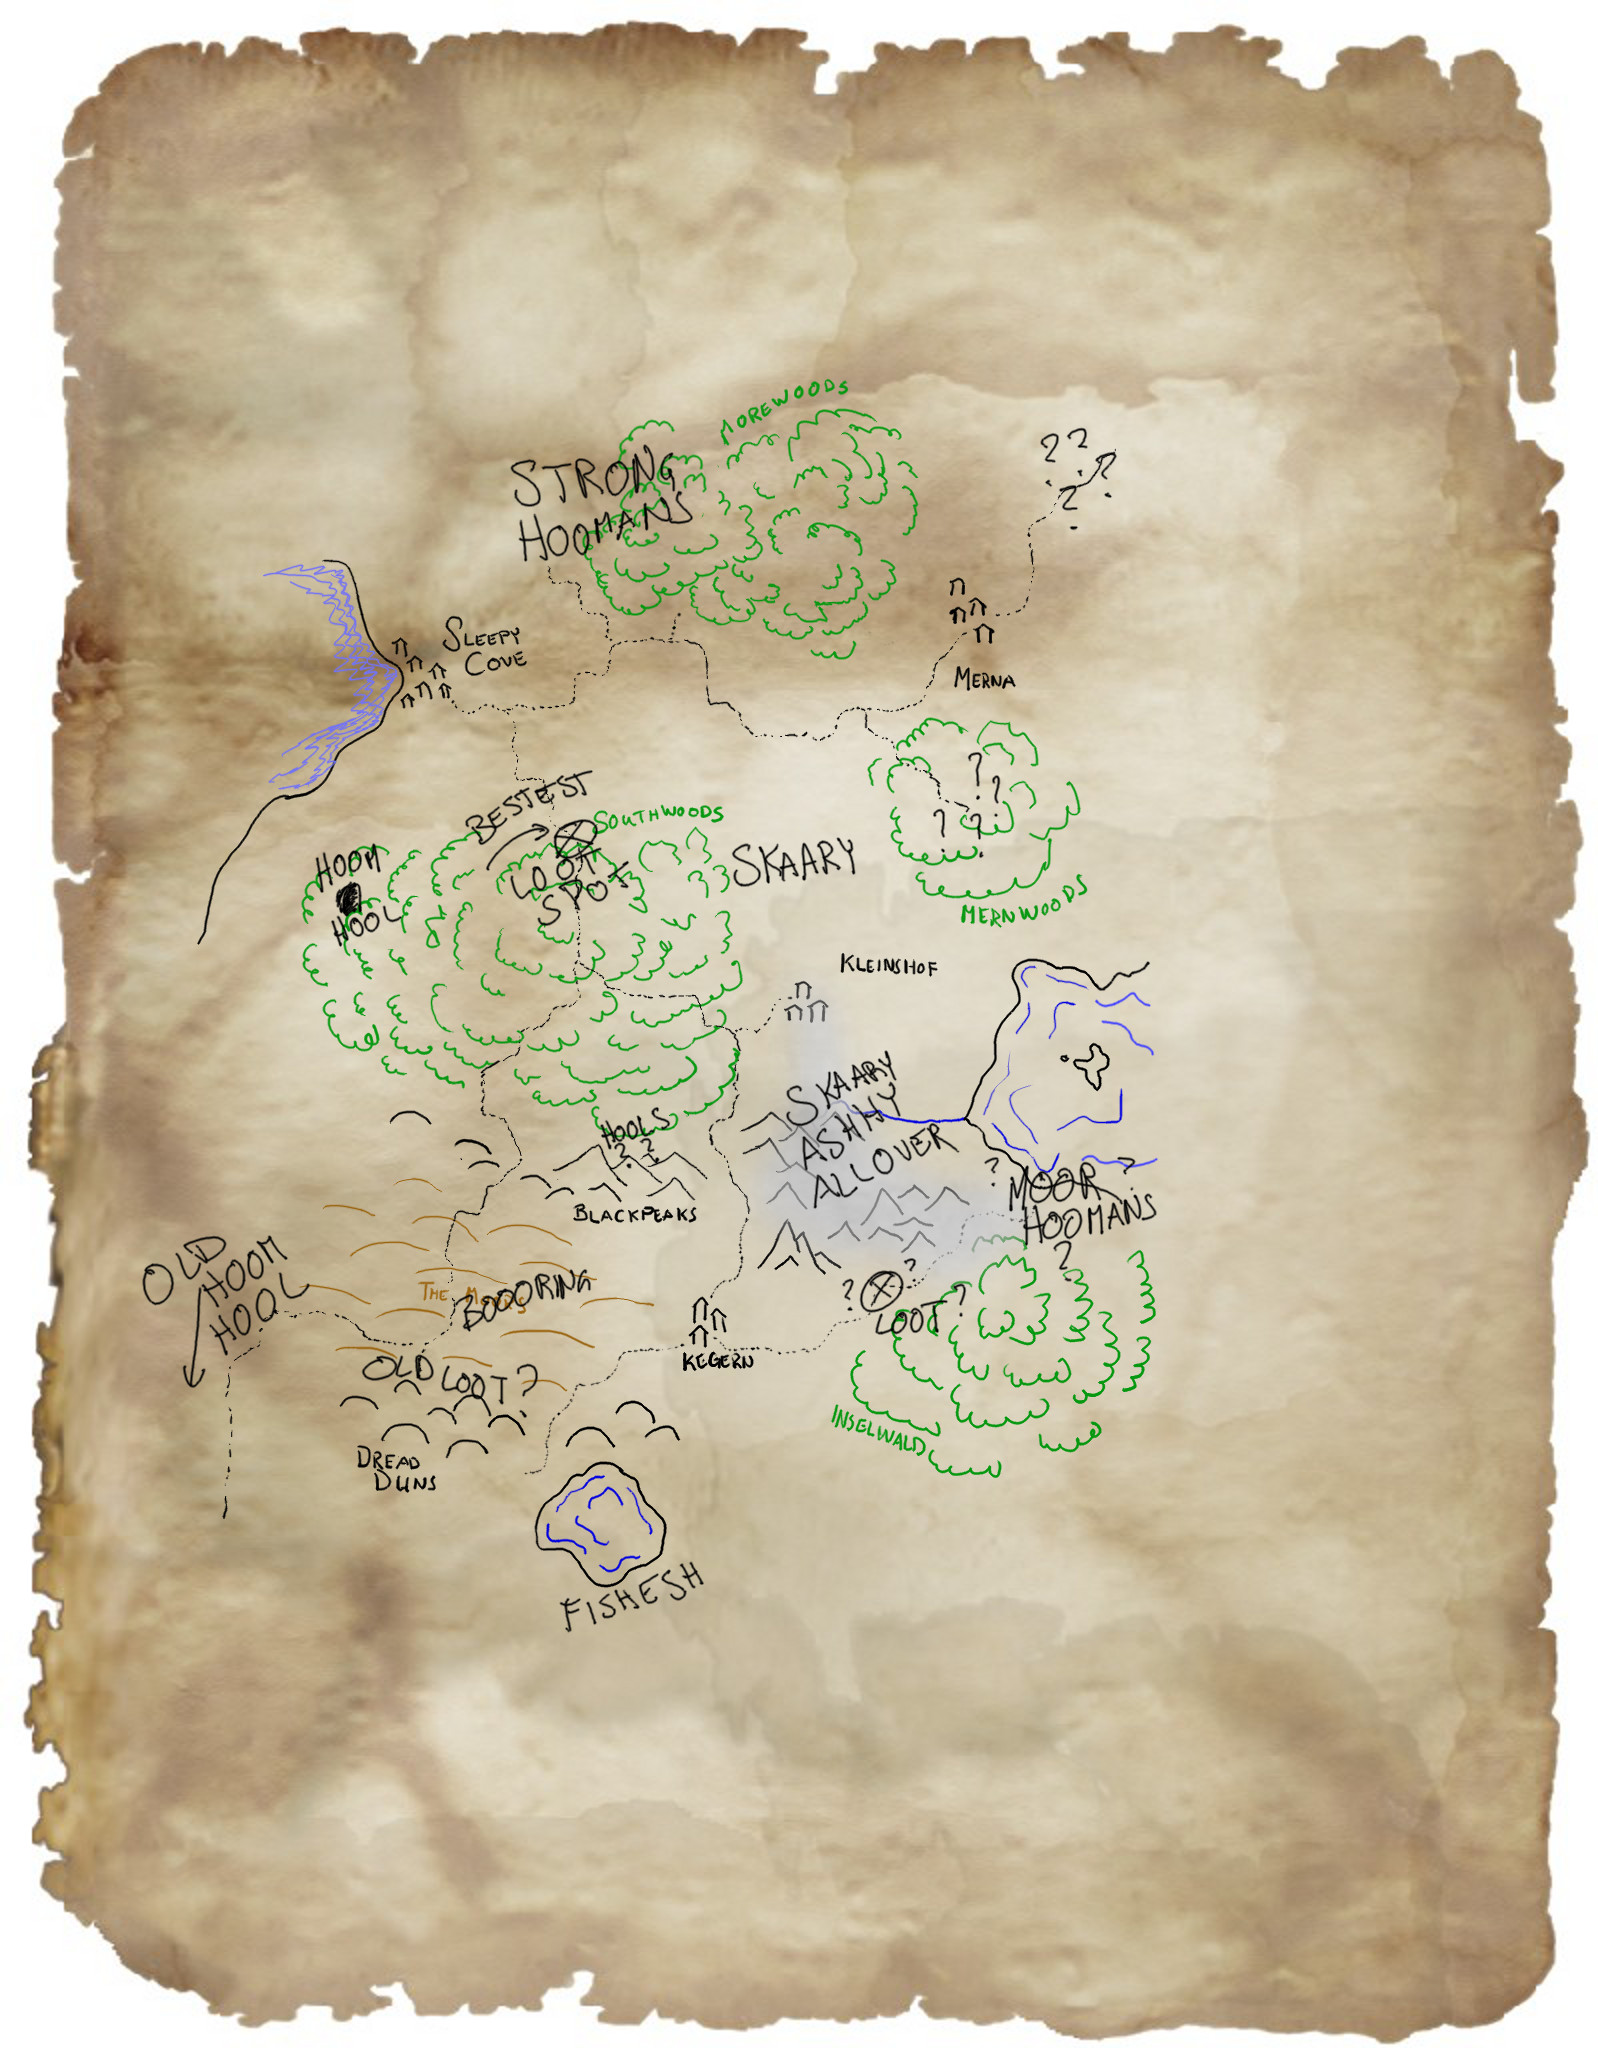
\includegraphics[width=0.999\textwidth]{fig/region.jpg}
  \caption*{The local region, as known by GamGang}
\end{figure}

In short: Hoom Hool sits in a rich forest where even an inept and lazy bandit gang can forage and hunt for around 50\% of their food. Nearby is a good ambush spot along a trade route from Sleepy Cove harbour to Kleinshof and Kegern. The Gang has settled in since a couple of weeks and done one quick highway raid at the Bestest Lootspot already. The region map shows what the goblins know of their new surroundings, though nothing outside Hoom Hool, Bestest Lootspot, and their immediate surroundings has been scouted yet.

The region is under rule of Baron Evilnius Conq. He has light patrols out keeping the peace after the \emph{unfortunate} incidents a while back where he employed evil demon magic to topple Baron Pawa. There are still some demons and monsters roaming around in the aftermath of the whole Uchly Namen rampage. And then there was this sorcerous plague in the south east which turned the land grey and ashen. Other than that it's a good place to live. \textit{See the earlier campaigns and adventures like \texttt{Return of Uchly Namen} and \texttt{Edwin the Chromophobe}.}

Apart from some loose demons and monsters there are no bandits in the general area around Sleepy Cove since the previous Heroes took care of both the SouthWoods goblin bandits and the Eisenkrafs bandits during the \texttt{Return of Uchly Namen}. So when GamGang starts up they find a fairly relaxed populace to prey on. Demons usually eat lonely traveller rather than wagon caravans.

Robert the Reeve is the lawman in charge of keeping the peace around Sleepy Cove, Merna, Kleinshof. He is efficient but selectively corrupt. The Heroes can run into his patrolmen when they travel the wild or visit a village. Any survivors of the goblins' banditry will be screaming bloody murder in the various villages and put all patrols on alert for the villains. If any of the Heroes are particularly memorable in appearance they will be recognised if they enter a village or encounter a patrol, but usually goblins all look alike to humans and people will normally not assume that every bunch of goblins encountered are the Beastly Bandits that the neighbours have been talking about.

Goblins are generally treated well in the region as long as they are part of society; follow the law and don't eat any babies. They are welcome in the villages if they dress well, behave, bring some commerce, and try to speak common tongue.

Note that villagers will generally recognise locally stolen property. If the Heroes loot a wagon going from Kleinshof to Sleepy Cove, then try to sell the stuff back in Kleinshof, odds are good someone will notice and tell the patrols. The villagers also have a chance to recognise donkeys, wagons, etc originating from the village even if the goods come from somewhere else. Patrol horses, armour, weapons etc are also easily recognisable, leading to questions.
\textit{I swears it! That stupid donkey we took just wandered off to a farm in the village. And woddunt-ya-now, the farmer said it was his, and that we had stole it from him! And then 'em soldiers came runnin'.}

\subsection*{... and how it changes}

As the goblin banditry escalates, Robert the Reeve will send patrols to try to find them. Any survivors might join and help out as well. If Hjalmar Hjälte survives the first fight he will gather survivors and mercenaries on his own, and he is good at tracking the GamGang both to their Hoom Hool and any other camp they might set up in the region. Remember that survivors also get xp, so have them level-up, buy gear, and rent hirelings suitable for revenge.

As the goblins ambush, raid, pillage, etc throughout the land they will become known and the people in the villages will learn what they look like. Trade convoys will be guarded. Patrols will flee and call in the cavalry. The village militias will be armed and manned.

When it becomes evident that the patrols can't keep the land safe, Robert the Reeve will ask Baron Conq to send the Burmak Squad to root out the Goblin Bandits. If they fail the task will fall to Captain Lundqvist to take care of the problem once and for all. GamGang might beat Burmak, but Lundqvist will eventually stand victorious and force them to flee. If they beat Lundqvist once he will come back again later with a stronger force.

Relocating gives the gang a bit of respite, but only until they start their banditry again. As soon as they show themselves the hoomans will try to track them down. At this point the region is too difficult for a bandit gang and it's time to finish the campaign soon. Throw in a side adventure, perhaps, then send them on to GrimGnash.


\subsection*{General path through the campaign}

First get the players accustomed to their new goblins by having a couple of robbery fights. \hyperref[00justanotherdayattheoffice]{\texttt{Just Another Day at the Office}} and \hyperref[01robberygonewrong]{\texttt{Robbery Gone Wrong}} introduce \hyperref[hjalmarhjalte]{Hjalmar Hjälte} and \hyperref[sturskurkboss]{SturSkurk}, and set the Dread Prophecy of \emph{Death by GrimGnash} rolling.

As time goes on the GamGang becomes more known in the region, more patrols and more caravan guards show up. Villagers have a higher chance of recognising the Villainous Goblins making trade harder. Hjalmar Hjälte, if surviving, will lead the early attempts to find and hunt down the Goblins. He gathers survivors, patrolmen, hirelings, etc, into militia or posse groups.

GammelTant will push for Revenge against SturSkurk: \hyperref[02killthebandits]{\texttt{Kill the Bandits}}. Sooner or later the Heroes will have to go kill him. Push the players to insert short intermission adventures here and there to get variation between banditry.

After a while the Law of the Land will send military squads like \hyperref[appendixburmak]{Burmak} and \hyperref[appendixlundqvist]{Lundqvist} to combat the bandits. The hoomans will track the goblin bandits back to base, forcing them to \hyperref[03defendhoomhool]{\texttt{Defend Hoom Hool}}. The soldiers could also follow up on patrol or caravan sightings and ambush in the open or other adventure locations. Burmak will be difficult but beatable. The only way to survive Lundqvist is to eventually \hyperref[04fleeandrelocate]{\texttt{Flee and Relocate}}. Lundqvist and his men will never give up. If defeated they will return in greater numbers. Captain Lundqvist is a legend, and near impossible to kill.

Forced to relocate, the \hyperref[appendixmountaingoblins]{BlackPeak hools might do, if they first kill or assimilate the goblin clans already living there}. The old Edwin Chromophobe dungeon should be mostly empty? A forest camp in MernWoods or the tower ruin in the MoreWoods perhaps? The old ruin on the Moors can work, but orc warbands will come and fight them for it. They could even try to live out of \hyperref[appendixtorturedungeon]{the old torture dungeon in the Dread Duns...} If they learn how to operate the meckanickery.

With the region armed and on alert, and the military hunting them as soon as they show themselves, life will get progressively more difficult for the gang. Soon it's time to wrap up the campaign. Prepare them early. Start having GammelTant scare them with GrimGnash horror stories early, a few days after Gamling has died. Have scout groups and foraging parties disappear occasionally. GammelTant will get more pushy for them to attack GrimGnash as time goes by. Don't drag out the campaign too long. When it's time to end, if they still don't want to go and GammelTant can't make them, GrimGnash will come calling when they are out travelling or at another adventure location. \hyperref[05deathbygrimgnash]{\texttt{Death by GrimGnash}!}.

\

The players have a lot of choice in what they do and when. Make sure they find the treasure map to the torture dungeon early on. While travelling they will see the IffyGriffs far away. Soon the mutated runts will show up and they can lead the way to the magic stream. Throw in patrols, traders and travellers, etc, as suitable. Simple things like going shopping can turn into adventures if someone in town recognises stolen merchandise or goblin bandits, perhaps a patrol group is resting at the local inn? A village might hire some warriors to clear the bandits or guard the town or caravans. The Heroes might get tired of GammelTant? Let them try to seize power.

\

Regardless, 
\hyperref[02killthebandits]{get them to attempt an attack on SturSkurk before 150xp}. 
\hyperref[03defendhoomhool]{Send Burmak at them before 250xp}. 
\hyperref[03defendhoomhool]{Lundqvist should make a first attack before 350xp}. \hyperref[05deathbygrimgnash]{Finally, make them face GrimGnash before 500xp}.


\subsection*{Recommendations on XP}

Setting a baseline of 5xp per session to all active Hero characters for the campaign gives a slow steady progression even if the battles are slow and the opposition xp share per Hero is small. I would deduct this from the specified "adventure xp". E.g: an adventure specifying a baseline 15xp each with 8xp bonus for successfully finding Thingamajig would pay out 5xp to each character for each of the two sessions it took, plus 5xp to each character upon completion for the rest of the "adventure xp" and 8xp each since they managed to find Thingamajig. Then another (e.g.) 34xp to share between the characters for the opposition they scared off, killed, befriended, or snuck around. If the same adventure took four sessions I would still pay out 4 * 5xp for the sessions, no extra xp for adventure completion, full 8xp for Thingamajig and split the shared XP for the opposition as normal.

In the playthrough the Heroes went from ca 100xp to ca 500xp over 44 sessions. Since I used a baseline of 5xp per session it means that more than half the total XP came from session XP rather from achievement or opposition XP. Not great perhaps, but it wasn't obviously visible to the players and it created a slow steady progression with a few spurt boosts here and there when they completed major milestones, or did something clever, funny, or cool.

Note that, apart from GrimGnash, this campaign has nothing relevant intended for a dozen half-k Heroes, so tie up the story around there, if not before. 








\clearpage
%--------|---------|---------|---------|---------|---------|---------|---------|
%       10        20        30        40        50        60        70        80
%-------------------------------------------------------------------------------
\phantomsection\addcontentsline{toc}{section}{00 just another day at the office}
\section*{00 just another day at the office}
\markboth{just another day}{just another day}
\label{00justanotherdayattheoffice}

This is a simple intro fight to get the Heroes tested out, so it's business as usual. Go to the twisty bit of the road and wait for the wagons. Capture some loot and get rich. Cook a tasty Victory Stew from the corpse of an unfortunate farmer.


\subsection*{synopsis}

Travel to the Bestest Loot Spot, set up an ambush, fight the wagon train. Probably get at least some loot even though most of the opposition will escape. Go home and celebrate.


\subsection*{adventure}

Gamling sends the Heroes to do a robbery on their own. They cannot bring any other goblins, wolves, etc from the camp. The Heroes have to fight as they are rolled up and with their starting gear.

\begin{readoutloud}
\emph{[Gamling speaks:]}
Yoo faitas! Yoo go hunt food! We hungry! Me Bizzi! Run get loot at Bestest Lootspot.
\end{readoutloud}

\noindent The Heroes can pick up some minor equipment from the camp, but not much of value. They can't go buying anything new before this first mission either. If they want to bring something of value from the camp have them argue with Gamling about it. Haggle, Leader, or any fancy intelligence based arguments won't work since Gamling will just smack them with superior strength and fighting skills. Instead have a psy-vs-psy nagging argument modified mod-1 for every 10c value they want to bring. If they fail-3 then Gamling will smack the arguing Hero until he shuts up, doing 1hp damage per nag roll. If the Heroes are cheeky and want to roll for defence, allow them at mod=0, just regular light brawling, but if they succeed Gamling gets angry and will try to smack them harder, actually landing a real brawling fist attack. Continue until they give up or flee and stay away for at least a few hours. Or, why not have a tiny fight? Impromptu 1v1 with lots of others cheering on? Gamling won't kill anyone on purpose though. Ganging up on Gamling will bring the whole clan down on them and it will be time to roll new Heroes.

The camp has only a few days worth of food, some torches, a few extra knives, staffs, clubs, shitty spears, rusty axes, goblin short bows, etc. A few hides, some rope, a handful of torches, and other simple equipment is also available. Most of the camp gear is mod-1 or 66\% abs or some such. It's good if they bring the camp's old donkey though, since it can carry a lot more loot than the Heroes can. But let them think of it themselves. Gamling will scream at them when they get back if they forgot it. GammelTant will kill and cook one of them if they loose the donkey though.

The wagons only move during the day so no use bringing night fighting gear. They can of course be sneaky and try to seek out the wagons during the night if they want. They need enough track skill or actually move the party onto the wagon night camp to find it. The wagons travel from Kleinshof to Sleepy Cove, which at 10 leagues per day (10sq/d) takes two days. They camp for the night just north of the trail fork. A lightly forested area with a wagon circle and tents, fire pit, lookout, etc.

Have the players set up the robbery as they please. They have plenty of time to prepare. If any of them pass int rolls you can helpfully suggest things like: \emph{If you'd had anyone with the skill "traps" you could have set traps by the road...}

When the players are finished, start the fight by having the wagon train move onto the map, wagon by wagon over a few rounds. Hjalmar Hjälte leads the train, walking a few squares in front of the first wagon.


\subsection*{map mechanics}

The route along the road is almost 100sq long. Assume the wagons moves at a safe 5sq/r (slow run) after being attacked. That gives 20r for the GamGang to force them to stop before they leave the map.

One way to get more time is to barricade the road with a tree, stones, angry goblins, etc. They can also try to break one of the wagons, or kill a donkey to have the wagon stop at a difficult to pass spot, or some such. But don't hint at them to barricade the road. More fun if they for example have a running fight, chasing the wagons through the map.

The wagons enter the map at speed 3, with 3-6sq empty space between them. Then accelerate to speed 5 when in a fight. The wagoneers and heroes have mod-3 to their perception rolls unless something indicates that there might be an attack incoming. Things like a tree felled over the road will indicate an attack and make them suspicious and careful. Same if they find goblins hiding or in plain sight.

The map has trees, bushes, boulders, etc. Should be plenty of good opportunity to hide, set up an ambush, take cover, etc.


\subsection*{opposition: wagons and Hjalmar Hjälte}

Stats for Hjalmar Hjälte is available in the \hyperref[hjalmarhjalte]{appendix} page \pageref{hjalmarhjalte}. Get stats for typical farmers, swordsman, archers from the rulebook, campaign section. Farmers ca 100xp, swordsmen and archers ca 150xp.

The caravan is led by Hjalmar Hjälte, a not too difficult hero, and guarded by Swordsmen (150xp) and Archers (150xp). Each wagon is driven by a farmer armed with knife or axe and each wagon has either a Swordsman or Archer walking alongside or riding in it.

Hjalmar Hjälte and one wagon should be enough to go against four goblins, then bring in another wagon for every two additional goblins. Recommend first two wagons have swordsmen, then one with an archer, then another archer or swordsman.

The wagons can go faster than 5sq/r but risk breaking down. For every speed step above 5 a wagon suffers 5\% chance per round to loose a wheel, overturn, etc. E.g. at speed 9 it's a 20\% chance per round.

If the road is blocked they will go into defensive position bringing the wagons together, phalanx fighters with archer support, etc. If the Heroes wait to attack (must pass psy or int rolls, goblins are impatient) the farmers will finally act to remove a road block or impediment, but will be guarded by the swordsmen and Hjalmar Hjälte.

If the farmers are loosing and can flee they will dump some loot and no longer suffer the risk of breaking their wagons when they go fast. Without loot a wagon can safely travel 10sq/r and the farmers are great drivers.

Hjalmar Hjälte will make simple attempts to coordinate with the swordsmen guards, and possibly the farmers, but nothing super clever. He will retreat and quaff if hurt. If he still can't win he will flee when almost dead.

Story-wise the best outcome is if Hjalmar Hjälte manages to flee together with some wagons. Then it's natural that he starts trying to gather a posse to go after the goblins a little bit later in the campaign.


\subsection*{loot}

The wagons have mostly food, simple materials, etc. Assume each wagon has total loot for around 10s, but nothing fancy. Just look through the price/equipment lists and pick a few items. E.g: 50x days food, 2x 10l kegs of beer, 6x blankets.\\
Each farmer has 1d3 silver and 1d10 copper.\\
Swordsmen and archers have 1d5 silver and 1d20 copper.\\
Hjalmar Hjälte have 3+1d5 silver and 10+1d20 copper.\\
Also nice if one of the wagons have a hidden bag of 10+1d10 silver (find mod+3 if they say they search the wagon and spend a few rounds, perception is not enough).

The donkeys are difficult to subdue since they don't like goblins. Requires a series of str vs str successes, or a smaller series of ride successes, or an animal command success per donkey. 

If they bring wagons when leaving it's slow going. The wagons only have 2 leagues cruise speed through forest, and require a successful ride roll per day to avoid getting stuck or damaged by terrain if not on roads.

The loot cannot be sold in Kleinshof since that's where it comes from. The wagons or donkeys cannot be sold in Kleinshof, Sleepy Cove or Kegern. The villagers will recognise the donkeys or wagons and have Conq Solders arrest the Heroes for thievery! Interesting little side adventure if they try.

Note that Gamling and GammelTant will take any money and loot not hidden away and put it to the Coffer. The players should figure out their stories beforehand if they want to sneak something past the loot collector when they return, or they all have to pass int rolls to not let something slip and squeal. This will be the same for the return of every adventure as long as Gamling or GammelTant are alive.

\

The adventure is worth 10xp each, and shared opposition xp. Add another 5xp each if they do a clever ambush, or something fun.











\clearpage
%--------|---------|---------|---------|---------|---------|---------|---------|
%       10        20        30        40        50        60        70        80
%-------------------------------------------------------------------------------
\phantomsection\addcontentsline{toc}{section}{01 robbery gone wrong}
\section*{01 robbery gone wrong}
\markboth{robbery gone wrong}{robbery gone wrong}
\label{01robberygonewrong}

Business as usual. Go to Bestest Lootspot and wait for the wagons. Capture some loot and get rich. The problem is that the SturSkurk gang shows up and Gamling gets killed. This is the start of \emph{Goblin Destiny: Death by GrimGnash}.


\subsection*{synopsis}

GamGang prepares a highway robbery. The wagon train enters and the fight starts. Soon the SturSkurk Gang enters the map. Gamling charges SturSkurk Boss and quickly dies. Rest of GamGang flee the fight soon thereafter, grabbing minor loot. It is unlikely but not impossible to beat both the wagon train and the SturSkurk Gang.


\subsection*{adventure}

The food from the previous raid is gone, and the GamGang is starving again. Must have more food! More Loot! This time Gamling himself will lead the outing.

\begin{readoutloud}
\emph{[Gamling speaks:]}
Em faitas! We go hunt moar loot stuff! Grabba em spearsanswords! Hurtysticks for all! Waik em shootas. To e twisty bit we go. Tiny Looka has seen beeg wagon komma! Lotsa loot! Go! Go!
\end{readoutloud}

\noindent Since Gamling is with them they can also add some support goblins. A couple of disposable warriors or fighters, as long as they can all travel fast enough on the region map. The camp is soon hungry again! Gamling will allow at most five days away: two days to Bestest Lootspot, one day for the robbery, two days home again. This means a minimum of four leagues per day. Any goblins who can't keep up should buy "travel" or suffer as Gamling will force march the group. Every lacking league gives the slow-poke 1hp damage and max stamina -1 until home again and rested.

Allow the players to position and prepare for the robbery. But it can't be too clever or Gamling will scream at them to do it differently.

The wagons arrive and there is some fighting, the heavy wagoneer should be an issue. Keep Gamling somewhat near the map border where you plan to have SturSkurk enter. Once SturSkurk arrives Gamling will charge him and die quickly. After Gamling dies SturSkurk will fight both the goblins and the wagon train. The goblins are more of a threat so SturSkurk will focus on them first, unless it costs them loot opportunity.
GamGang should be forced to flee soon after Gamling is slain. Perhaps they pick up some loot along the way.


\subsection*{map mechanics}

Same as before, see the map mechanics section under the previous adventure. But this time Hjalmar Hjälte is not with them even if he survived the last encounter. Instead the wagon train has the heavy Wagoneer at the end. His armoured-illers can clear road blocks to some extent and push carts or bandits out of the way to allow for escape.

As soon as the fight with the wagons has started properly the SturSkurk Gang will arrive. Gamling charges SturSkurk and his two orcs. Make sure Gamling dies in a couple of rounds. Gamling won't defend, just attack all out with his axe. SturSkurk will play it safe and use his black cat and luck to make sure the dice against Gamling fall the right way.


\subsection*{opposition}

With first the farmers and Wagoneer, then the SturSkurk Gang, it is unlikely that the Goblins will win this fight. Try to balance so that the players feel it really is \emph{very dangerous but not impossible} to beat both the wagon train and SturSkurk Gang. It is possible to get the SturSkurk Gang to fight the wagon train, and carefully pick off some of the people on both sides until the rest of GamGang has a chance to win.


\subsection*{opposition: wagons}

The heavy Wagoneer counts for 2x goblins. For every further 2x goblins add another wagon with guard. Use archer guards and get the farmers to escape as soon as possible.

The heavy Wagoneer comes last in the wagon train. If the road is blocked his armoured-illers can push aside other wagons, or perhaps even a tree if they have some time. The Wagoneer will fight if necessary, but will try to just escape.

The farmers will try to escape, including turn around if it seems to help. Archers can fire from wagons with mod-3.


\subsection*{opposition: SturSkurk}

This is not the full SturSkurk gang, the rest are back at the camp. Adjust as needed. SturSkurk Boss, 2x front line melee orcs, the witch, 3x archers goblins.

The SturSkurk gang enters the map in staggered group. Main melee line phalanx, the witch in between, then archers group behind.
They will start to attack the goblins, but will also attack farmers and the Wagoneer if they can snag some loot.

SturSkurk will fight and kill Gamling first, since Gamling will charge him immediately on arrival. The melee phalanx line will protect their archers, and only push into the fight if their archers are not strong enough to win a shooting duel.

Main melee front line is SturSkurk Boss with the two orcs on either side. They move together and fight defensively, primarily mainly making sure that the opposition get pinned in place so their archers can whittle down the outliers. When Gamling charges Boss will block and let the orcs stick him to death. If Gamling leave an opening Boss and Orcs will be merciless.

The Witch will shock bolt and cast slow on Heroes when possible to aid her melee line. She will do this on Gamling immediately when he charges. She will also run up and use ward shield on the boss and orcs if necessary. For self defence she'll use fire storm.

The SturSkurk archer group will run around to stay out of reach and pepper arrows when possible to suppress Heroes' archers and casters.

If it's obvious that they will loose then Boss will order a retreat. He does not want to loose his fighters here.


\subsection*{loot}

The regular farmer carts have similar loot as in Just Another Day at the Office, ca 10s worth of food and simple items.\\
The heavy wagon is a small camping house and has 100+1d100 days' food, ca 20s of random trade stuff, and a couple of high end items e.g. Quaff!. It also has a small stove, some cooking gear, a few days of good food, minor trinkets, clothes, etc. In a \emph{hidden compartment} in the wagon is 20+1d10 silver and 50+1d50 copper (find roll required mod-0, can't find with perception roll).\\
SturSkurk people have just 1d3s + 1d10c each. Their gear is in ok condition.

If the Heroes flee, perhaps SturSkurk Blue Boss takes Gamling's big 2h axe as a trophy? It also has a sales value so they wouldn't leave it behind.

\

Award ca 10xp each for the adventure, and shared xp for the defeated opposition. Don't deduct if the Heroes flee. They are supposed to run away here. Add another 5xp each if they force SturSkurk to flee, and another 5xp if they manage to stop and loot the heavy wagoneer, and 3-5xp if they manage to get away with at least some loot.

\

This is a good place to have the Heroes find  
\hyperref[appendixtreasuremap]{the treasure map to the Dread Duns,} 
leading them to 
\hyperref[xxtorturedungeon]{the Old Tower Ruin and the Torture Dungeon below.} 
It can be stuffed in a hidden compartment in a wagon, stuffed in the shirt of a corpse, or hidden away in the Wagoneer's coin stash.





%-------------------------------------------------------------------------------
%formatting: flush to bottom of page, or top of next empty page.
\vfill
\needspace{12\baselineskip}
\section*{Gamling is Dead, all hail GammelTant!}

After Gamling has died GammelTant will be furious for a bit, call for revenge, and send Hemskelina to scout for the SturSkurk gang. Soon she remembers the Old Prophecy of \emph{Death by GrimGnash}, and locks herself away with her crystal ball.

When Hemskelina comes back reporting of the SturSkurk bandit camp location GammelTant sends the Heroes to kill them all and steal all their shit. And of course to bring back the corpse of the Blue Boss so she can cook a Victory Revenge Stew!










\clearpage
%--------|---------|---------|---------|---------|---------|---------|---------|
%       10        20        30        40        50        60        70        80
%-------------------------------------------------------------------------------
\phantomsection\addcontentsline{toc}{section}{02 kill the bandits}
\section*{02 kill the bandits}
\markboth{kill the bandits}{kill the bandits}
\label{02killthebandits}

The camp of the SturSkurk bandits has been found by Hemskelina. It's time to kill them all! And eat the good ones.
Make GammelTant force them to attempt killing SturSkurk at least once before the Heroes reach \textbf{150xp}.


\subsection*{synopsis}

Scout the SturSkurk camp. Assault in darkness. Kill the SturSkurk bandit gang. Grab SturSkurk Boss' corpse for GammelTant, at least the head. If fail, try again later on.


\subsection*{adventure}

The Heroes are responsible for planning and execution. Hemskelina is coming along but will not fight as a lead figure. Her task is to kill SturSkurk Blue Boss if he tries to escape.
The Heroes can bring a couple of fighters, warriors, runts, and a wolf if they want.

\begin{readoutloud}
\emph{[GammelTant shouts:]}
Go Get Em Killt! Blue Boss bring back! Kook-em corpse in Victory Revenge Stew I will! Take-a em few warrjas and faitas with-ya!
\end{readoutloud}

Hemskelina will have scouted the outskirts of the camp but not the interior. Provide limited view into the camp from a few vantage points. The Heroes can see the outline of the camp but not all of the the interior.

SturSkurk gang has have a competent scout on guard patrolling the camp. Hemskelina can track him but need help to kill him quickly.
The Heroes can position and prepare for the camp assault but they cannot dig trap pits or do similar heavy work/noise activities in the area without getting spotted. 

\

This should be a tough fight. The Heroes might fail their first attack and have to come back later with a better plan, or find some help. Make sure to force the Heroes to attack SturSkurk early in the campaign, before they have become too powerful.


\subsection*{map mechanics}

Apart from a couple of goblin fighters and a camp babe by the fire, the bandits are sleeping hidden in their tents, not visible from the outside. Two dogs are sleeping by the fire and two more elsewhere in the camp. They wake easily (per 12).

The scout on patrol outside the camp palisade slowly and carefully sneaks around, and he's a competent scout. Either kill him or time the setup and assault so the scout can't see it. Hemskelina will keep approximate track of his expected whereabouts, but that's not 100\%. If the scout sees anything he will sound the alarm immediately, then try to gather info on the size of the enemy force and signal the gang if possible.

As soon as intruders are detected the whole camp will immediately wake up and start emerging from their tents to fight. It takes each bandit 2+1d3 rounds to wake up, grab weapons, and emerge from their tents.


\subsection*{opposition}

For the \hyperref[01robberygonewrong]{\texttt{Robbery Gone Wrong}} fight there is probably just the boss, 2 orcs, witch, 3 archers. For the assault here the rest of the SturSkurk Gang is available, minus those that were killed in the previous episode. The full gang is the boss, the witch, 2x orcs, 4x archers, 4x spear men, 2x scouts, 2x goblin fighters, 3x camp babes, 4x dogs. Adapt to suit your players. 
\hyperref[appendixsturskurk]{See the SturSkurk appendix for stats and info}, page \pageref{appendixsturskurk}.

SturSkurk gang doesn't have anyone with medical or magical healing skills. Their wounds will heal at normal speed, and they can't easily recruit more people quickly. If GamGang is quick, SturSkurk gang will still be wounded from the previous fight when the Heroes assault the camp. 

The gang is not suicidal. They will fight hard and take some losses, but if they can't see victory they will grab as much of their treasure as they can and flee to regroup later. They can always come back for revenge later, and take back what gets stolen.


\subsection*{assistance ?}

A clever idea could be to go to one of the villages nearby and talk to a patrol soldier about \emph{"this nasty bandit gang in the forest camp over there"} and have the soldiers fight SturSkurk. But SturSkurk is also somewhat smart, he has already bribed Robert the Reeve, the lawman in charge of the region between Sleepy Cove and Kleinshof.

For this to work the Heroes can go further North to Baron Conq's castle up in \emph{Strong Hoomans} territory and talk directly to the military leaders like Burmak or Lundqvist, strong merchants, or some such. And they must be pretty convincing to be able to get someone to look into it.
The heavier military groups like Burmak and Lundqvist don't take orders from Robert the Reeve. But normally the military will respond that it's the Reeve's responsibility and not theirs.

SturSkurk have already bought selective blindness from Robert the Reeve so the Heroes can't hint/convince/bribe him to order patrols to attack SturSkurk. No patrol leader will bring his group to fight SturSkurk camp knowingly without direct orders from the Reeve. But give the Heroes some xp anyway if they try to persuade the law man.

\

One trick that could succeed though is if they manage to entice a patrol group into pursuing them directly into conflict with the SturSkurk gang in their camp. The patrol officers don't know that SturSkurk have bought safe harbour from Robert the Reeve. The Heroes can also pick up a posse gang or similar to pursue them to the bandit camp and bring them into confrontation with SturSkurk camp. \hyperref[playthroughkillthebandits]{This is how it was done in the playthrough}, page \pageref{playthroughkillthebandits}.


\subsection*{loot}

SturSkurk camp has quite a bit of practical loot, and a bit of treasure if the Heroes can find it before someone in the SturSkurk gang flees with it. The corpses are good for eating and their weapons and equipment is of decent quality. 
\hyperref[appendixsturskurk]{See the SturSkurk appendix for a loot list}, page \pageref{appendixsturskurk}.


The camp site itself is also easy to defend and has three ways out if assaulted by a superior force. It's not a bad place to settle GamGang if Hoom Hool is lost.

\

Reward 15xp each for taking out the SturSkurk Gang. Another 5xp each for killing or capturing SturSkurk Blue Boss. Any clever way to have a third party help in the fight should give 10xp each. Then split the opposition xp as usual.

\

If the Heroes haven't found it yet, this is a good place to have them find 
\hyperref[appendixtreasuremap]{the treasure map to the Dread Duns,} 
leading them to 
\hyperref[xxtorturedungeon]{the Old Tower Ruin and the Torture Dungeon below.} 
SturSkurk might have it in his tent, or locked away in his treasure chest.


\subsection*{followup}

If SturSkurk flees he may want revenge. If they flee with enough treasure and people left they will form up, scout, and sneak up on Hoom Hool later, or lay an assault along a travel route, or attack when the Heroes are coming up for air after some hard fight, already wounded.

\

At this point it's good to remind the Heroes of the Looming Doom. Death by GrimGnash. GammelTant has spent many late hours gazing into her crystal ball. She has seen Teeth and Claws kill all the goblins over and over again. Still she has no clue who, where, or even what GrimGnash is. Just large teeth and huge claws, and lots of dead goblins. 

Still she will insist that the only way to avoid total death of whole GamGang is to kill GrimGnash before the prophecy comes true! She will remind them often and try to get them to also gather info themselves on who GrimGnash might be, and where.














\clearpage
%--------|---------|---------|---------|---------|---------|---------|---------|
%       10        20        30        40        50        60        70        80
%-------------------------------------------------------------------------------
\phantomsection\addcontentsline{toc}{section}{03 defend Hoom Hool}
\section*{03 defend Hoom Hool}
\markboth{defend Hoom Hool}{defend Hoom Hool}
\label{03defendhoomhool}

Sooner or later some gang of hoomans is going to track the goblin bandits back to Hoom Hool. The approximate location is already known to the law, as it was previously home to another gang of goblin bandits. See the historical campaign \texttt{Return of Uchly Namen}, adventure \texttt{The Red Stone}, where the Heroes of the time are tasked to clear out the previous occupants of Hoom Hool in search for the lost Jewel.

Plan the assaults so you can 
\hyperref[appendixburmak]{throw Burmak at them before the Heroes reach \textbf{250xp}}, and 
\hyperref[appendixlundqvist]{Lundqvist should attack before \textbf{350xp}}.

\

\noindent\textbf{Note:} This adventure is not necessarily aimed at Hoom Hool. Perhaps GamGang has already settled somewhere else? Then let the hoomans attack there. The main goal of the hoomans is to weaken GamGang, force them to flee somewhere else, away from looting and banditry, to stop them preying on the region's civilians.


\subsection*{synopsis}

The Law of the Land attacks Hoom Hool to drive out the Goblin Scourge. If they fail they will come back later and try again, with a stronger force. At some point GamGang must flee, continued in \hyperref[04fleeandrelocate]{\texttt{04 flee and relocate}}.


\subsection*{adventure}

The hoomans have found Hoom Hool, and now they attack. This adventure will probably happen more than once before GamGang is defeated and flees.

Most likely this will happen once or twice. Perhaps a surviving Hjalmar Hjälte gathers a posse and make a doomed attempt to take revenge on the Goblins. This should be beatable without too heavy losses.
Later on Burmak will attack. This is supposed to be difficult but the Heroes should win.


\subsection*{map mechanics}

This is where it pays to have fed the gang well. The more food there is the fewer goblins are away out in the woods foraging for food. If the goblins are well fed and the larder stocked then the whole gang can be in the camp at full strength. If they are starving then as many as 75\% can be away in the woods when the attack comes.

Start out with most goblins present out in the camp. Then let them either scatter and flee, or retreat to the cave for a more defensible position. Once in the cave though it's easy to get cornered, but the T section behind the entrance is a good place to counter attack the intruders from two fronts and perhaps split them and force them into a corner.


\subsection*{opposition}

First gang should be a posse or militia group made up of survivors. E.g: Hjalmar Hjälte or some other Brave Hero of the Land, out for revenge, or fame and fortune. Balance the group to be tricky but not too difficult. Assemble from survivors, standard civilians, common hirelings, and build a fun Hero or two to throw into the mix.
The attackers are not suicidal and should flee when it's clear they are loosing, bringing word to Robert the Reeve that a heavier force is needed.

Burmak force is the next step up. A cohesive military squad. They are much more difficult to fight and should be balanced to have a good chance of routing GamGang from Hoom Hool. See \hyperref[appendixburmak]{appendix Burmak for stats and info}, page \pageref{appendixburmak}

If Burmak fail, then Lundqvist will be tasked to finish up. His group is too difficult for GamGang to beat, and they will be forced to flee. See \hyperref[appendixlundqvist]{appendix Lundqvist for stats and info}, page \pageref{appendixlundqvist}.

If for some reason Lundqvist fails he will gather more soldiers and specialists and try again until he succeeds. And if GamGang kill Lundqvist, Baron Conq can always send for Sam Slick, Bling SwordSlash, or some other Major Hero to finally stomp out the menace.


\subsection*{loot}

The attacking force won't have much money on them. Their equipment is probably in good condition though, and their corpses should be excellent eating.

\

Surviving a posse attack should be 10xp each plus shared opposition xp. Burmak should be 15xp each plus shared opposition xp, and Lundqvist 20xp each plus shared opposition xp.


\subsection*{followup}

If SturSkurk is out for revenge, this might be a good time for them to strike, when GamGamg is either fleeing or wounded after repelling an attack.

At some point GamGang must relocate, continue with 
\hyperref[04fleeandrelocate]{\texttt{04 flee and relocate}}.












\clearpage
%--------|---------|---------|---------|---------|---------|---------|---------|
%       10        20        30        40        50        60        70        80
%-------------------------------------------------------------------------------
\phantomsection\addcontentsline{toc}{section}{04 flee and relocate}
\section*{04 flee and relocate}
\markboth{flee and relocate}{flee and relocate}
\label{04fleeandrelocate}

Another attack on Hoom Hool. This time the intruders are too strong. GamGang must flee and relocate somewhere else. Or perhaps the clever goblins have figured out that their current location will sooner or later get them dead since the hoomans know where they are, even if they have managed to survive the latest attacks.


\subsection*{synopsis}

One way or another, force GamGang to abandon their established location and move to somewhere less secure, further away from good banditry and loot locations.


\subsection*{adventure}

The hoomans are tired of the goblin bandits, and pile on increasing amounts of force to get them dead or gone. If GamGang make the move willingly they can move in an orderly fashion, in peace. If they are routed by force they must flee any way they can and probably scatter into the night, to gather later on, somewhere else.

\textbf{First:} escape, survive, regroup. If they are fleeing from a fight they probably scatter into the night. Some of them will be hunted down and killed, but most who make it off map will survive by hiding for a few days. Then they start gathering again, collecting escaped gang members over the next several days.

If they move willingly they just need to avoid getting ambushed when on the move and unprotected. Probably good to keep to the forests and hills as much as possible.

\textbf{Then:} find somewhere else to live. Where? SturSkurk camp is a decent spot but the Hoomans will find them there before long. Some other forest camp? Same again, the hoomans will find them. 
\hyperref[appendixmountaingoblins]{The hools in BlackPeak mountains are good spots to hide but already occupied}, page \pageref{appendixmountaingoblins}. 
\hyperref[appendixtorturedungeon]{The Torture Dungeon in the Dread Duns is out of the way but haunted by wraiths and infested by bugs}, page \pageref{appendixtorturedungeon}. 
The dungeon palace of Edwin the Chromophobe is probably still empty after the Heroes of Yore cleared it out in the earlier campaign adventure \texttt{Edwin the Chromophobe}?

It's a decent assumption that the Heroes will at least check out the BlackPeak hools if they haven't already done so. 


\subsection*{map mechanics}

They are probably leaving Hoom Hool, but look through the escape routes and situations for whatever location they are leaving. The attackers are not stupid and will try to kill off as many of the goblins as possible and will try to hinder escape.

Regardless of location, GammelTant will never leave her crystal ball. If they are loosing a fight and have to escape she will either run to get it herself, or send Hemskelina to do it. Hemskelina is an excellent sneak and can grab the ball and hide until the attackers have left and she can slink away.


\subsection*{opposition}

What will finally drive GamGang from Hoom Hool? Probably \hyperref[appendixburmak]{Burmak} or \hyperref[appendixlundqvist]{Lundqvist}, see appendices, pages \pageref{appendixburmak} and \pageref{appendixlundqvist}, and the previous adventure \hyperref[03defendhoomhool]{\texttt{03 defend Hoom Hool}}, page \pageref{03defendhoomhool}.


\subsection*{loot}

Whatever they can grab when they run away for their lives.


\subsection*{aftermath}

Settled somewhere else GamGang can start to rebuild. But as soon as they go out to resume their banditry the greater society of the region will start looking for them again, to hunt them down and kill them for sure this time. Perhaps the goblins can flee and relocate another couple of times but this quickly gets tiresome and boring.

It's better to push them towards facing GrimGnash than have them repeatedly fight for somewhere to live and food to eat.













\clearpage
%--------|---------|---------|---------|---------|---------|---------|---------|
%       10        20        30        40        50        60        70        80
%-------------------------------------------------------------------------------
\phantomsection\addcontentsline{toc}{section}{05 Death by GrimGnash}
\section*{05 Death by GrimGnash}
\markboth{GrimGnash}{GrimGnash}
\label{05deathbygrimgnash}


The prophecy comes true. Death by GrimGnash. No way around it. Here ends the campaign. Push them to face GrimGnash before they reach \textbf{500xp}.


\subsection*{synopsis}

Either they go hunt down GrimGnash where he sleeps in his lair, or GrimGnash attacks them somewhere else. Either way most die, some might flee to survive for cameos in later campaigns. If they try to attack then manage to flee, GrimGnash will sniff them out and retaliate very soon.


\subsection*{adventure}

GammelTant, or whoever is the leader at the time, sees Certain Death each night in the crystal ball and feverish nightmares. Huge Teeth and Claws rip the goblins apart. No matter where they move the Teeth and Claws come hunting for them. But still they don't know who, where, or what GrimGnash is.

\begin{readoutloud}
\emph{[GammelTant:]} Mussst go kill GrimGnash! Or it comes Kill Us All! Find it sleeping and Slay it Dead! Deader! Deaded for sure!
\end{readoutloud}

Sooner or later it's time to finish the campaign. If GammelTant is alive she will have visions of \emph{the Cave at the Highest Peak above the clouds, and the dark cave with the fiery light deep within}. If she is dead, give the new owner of the crystal ball \hyperref[coupaftermath]{the visions described in the aftermath section of the coup.} This should point them in the right direction. 

\

\noindent GrimGnash the Mighty Dragon sleeps in his lair in the highest peak, above the clouds, four leagues NE of Kegern. Best if the goblins find the lair and then attack when GrimGnash is asleep. GrimGnash can always attack them at any open sky map, flying over again and again torching them and whatever else can burn on their local battle map to crispy death and ash.

When he sleeps they can enter his lair and make some sort of clever attack. He will of course wake up and start killing the intruders.


\subsection*{map mechanics}

GrimGnash lair is split by a bottomless chasm. The walls can be climbed at mod+3. The platforms are elevated but not high and can be climbed in 1r at mod+3 or jumped in 3ap with a successful acrobatics-3 or jump-6 rolls. 

The huge northern flaming pyre vat braziers look different. Something is odd. When close (within per sq), roll per to notice that they look like they are alive and writhing. 
\begin{readoutloud}
The fire burning in the large pyres looks unpleasantly strange, flames moving around like they have a life of their own.
\end{readoutloud}
Casting ranged spells within the cave will spawn a fire elemental from one of the large pyre vats on the north section. Each pyre vat can spawn one elemental per round.

\

When entering the lair GrimGnash is asleep. He will wake from any loud noise anywhere in the lair. Any ranged magic being cast will spawn elementals and that will also wake him. Roll per-6 to see if he wakes up for anyone not sneaking when on the northern region, and per-3 for anyone moving on the dais section and failing sneak.


\subsection*{opposition}

GrimGnash himself and an endless stream of Fire Elementals that can spawn from the two large pyres in the north section of the map.

GrimGnash is a colossal (6x6) size monster with lots of hitpoints and thick scales, claws, teeth, tail, and fire breath. He's fast and can fly. At low hp he will regenerate slowly. He'll focus on high damage dealers and either swat them away or try to grab them and bite their head off. For multiple grouped attackers he will use fire breath or tail swipe. If in danger he'll fly to safety or simply rush through enemies throwing them aside.

Fire Elementals are simple. They will swarm targets and coordinate movement and attacks somewhat intelligently. They can move unhindered up and down platform edges.

See the \hyperref[appendixgrimgnash]{GrimGnash appendix}, page \pageref{appendixgrimgnash} for stats and details on both the Dragon and the elementals.


\subsection*{loot}

GrimGnash is rich, but he's also really vain. He's been spending most of his gold on giant skeletons, fake \emph{impressive}-looking treasure, large magical pyre vats, huge intimidating torches, etc. So there's not so much actual gold left, not compared to how the cave is decorated. 

Centre on the northern dais is a huge pile of treasure. Closer inspection will show that it's all fake giant stone coins with thin leaf gold surface polished to a perfect glimmering sheen.
All weapons found in the lair are of good quality, but enormous. They have never been used and are polished weekly. Assume 4x normal abs, requiring 10 + 2x normal strength, and suitably high damage potential. The scorched skeletons are well maintained and carefully posed, originally from enormous giants, 3-5m tall.

There is a treasure chest hidden in a niche in the north wall. Roll find+3 if searching the area, or per-6 if walking by when looking for loot. The actual coinage in the hidden treasure chest amounts to 50+2d50g in mixed denominations. The total cost of the strange decorations is sure to have run into thousands of gold. But who would buy it? Another odd Dragon?

\

Total xp to anyone who survives a full on encounter with GrimGnash should be 30xp each and permanent psy-1 nightmares. If they sneak out quickly give them 15xp and permanent psy-2. If they manage to slay the beast award another 10xp each and 100xp to share, and a permanent psy+1 self confidence boost. Slaying GrimGnash and boasting about it is also a quickly spreading permanent famous+3 bonus, \emph{if} they have something to prove the veracity of their tall tale.


\subsection*{prophecies}

GrimGnash is tired of prophecies. He figures in sooo many of them. And they make no sense whatsoever. Why would he go scouring the region hunting down some foul smelling goblins? He has better things to do. Nah, never believe in them.

\

But in this case... Mighty GrimGnash once lost a treasured bauble. The Shiny McGuffin was stolen by some Obnoxious Hero. Soon thereafter mr OH died, drowned in a stream in the forest a couple of leagues north of BlackPeak mountains. Time passed, as it does i stories. Then, by strange fate, the McGuffin started leaking warped magic, tainting and mutating the surrounding area. Anyone who has been there and got the taint will reek of it, reminding the Mighty GrimGnash of his lost Treasured Trinket. 

\

\begin{center}
\begin{minipage}[t]{0.48\textwidth}                   % [t] top align both boxes
    \emph{Alt, the Heroes find GrimGnash:}\\
    Then one day, whaddayaknow, he wakes from slumber to see a brace of goblins in his Lair, and they reek of taint. Reminded, his anger rises. He huffs and puffs and prepare to burn them all to a crisp!
\end{minipage}
\hfill
\begin{minipage}[t]{0.48\textwidth}                   % [t] top align both boxes
    \emph{Alt, GrimGnash must find the Heroes:}\\
    Then one day, when he's out flying low over the lands, he smells the taint. Reminded, his anger rises. He sees a group of goblins travelling the road below. He dives to attacks!
\end{minipage}
\end{center}

\

\noindent Or, if we twist it a bit:

If the Heroes decide to strike back first, and go murder GrimGnash just so he won't come murdering them, it turns out that GrimGnash had no clue about it all. He will at the next Boss Monster Social complain widely about the stupid goblins who crawled into his Lair and disturbed his sleep just because someone had gotten it in their head that he would kill them.

If, on the other hand, the Heroes try to avoid GrimGnash he will run across them one day and kill them all. Of course he will. He is destined to do so. Did they really think they could outrun destiny? And yet again he will complain to his Boss Monster colleagues that the Damned Destiny Writer is up to no good again, forcing him to go hunting when he would rather be sleeping...

\

\noindent \emph{Eh, what can you do?} 
















%===============================================================================
%                         I N T E R M I S S I O N S
%                         -------------------------



%%extra leaf, empty header, note of content
%%-------------------------------------------------------------------------------
%\clearpage
%\pagestyle{empty}
%\cleardoublepage
%\null
%\vspace{10cm}
%\begin{center}
%\emph{here ends the main campaign arc}
%\end{center}
%\vfill
%%-------------------------------------------------------------------------------
%\cleardoublepage
%\pagestyle{fancy}

















\clearpage
%--------|---------|---------|---------|---------|---------|---------|---------|
%       10        20        30        40        50        60        70        80
%-------------------------------------------------------------------------------
\phantomsection\addcontentsline{toc}{section}{XX patrols}
\section*{XX intermission: patrols}
\markboth{patrols}{patrols}


Patrols from the Castles or villages travel the lands to search for enemies, hunt bandits, and safeguard routes for travellers and merchants. The patrol soldiers are not automatically hostile. All depends on how well the goblins are known, what they do and how they are dressed when meeting, and what they are carrying.


\subsection*{synopsis}

When travelling they run across patrols. Talk or fight. Look and behave like civilians or fight like bandits. Small low level patrols are easy to trick unless anything "bandity" is obvious. They are also not that tricky to fight.


\subsection*{adventure}

Patrols are most likely along the roads, but will be out in the field as well. They usually don't enter the forests unless necessary.

\begin{readoutloud}
\emph{[Friendly Patrol Soldier speaks:]}
Hello hello there! How's life this fine day? Where are you fellows travelling this day? Anything interesting in those wagons? My dear wife is looking for some fine cloth for a new dress. Can you give me good price?
\end{readoutloud}

\noindent The Heroes need to either talk their way through the patrols by pretending to be traders, or bribe them, or fight them. The important part is to not allow any patrolmen on horseback to escape, which will immediately bring more soldiers down on them, as soon as they can muster and get there, usually within a day or two. And the soldiers bring trackers... The physical description of the goblins can also becomes known in the nearby villages.

If the goblins can pass for peaceful traders or farmers this is not an issue. If they start fighting and the soldiers are loosing they will try to flee, and one will take off on horseback to get help. Any soldiers on foot that manage to flee will try to follow the goblins at a safe distance (a few leagues behind), but only have limited track (3 or so).

Response groups can muster from Castle Pawa or Castle Conq and can travel up to 15 leagues per day. They will be 5-10 cavalry soldiers and have a scout (track 8) with them. They will likely be very quick to track down the goblins unless they can get into hiding quickly, or are very good at track or sneak to sufficiently hide their trail.

Civilian militia response groups can be called from any village, but will generally only be farmers, hunters, and a couple of hirelings. They travel at 8 leagues per day, and will have a good hunter (track 9) with them. A civilian militia group will not necessarily attack when they find the goblins. It may be enough that they track and stay nearby, to join with a later real military group.

If a civilian militia is raised from Sleepy Cove and Hjalmar Hjälte is alive, then he will join it together with any other survivors from the previous battles who happen to be available in the village.


\subsection*{map mechanics}

Just open field or plain. Add some rocks and trees, or old ruins, to make the terrain more interesting, but it should be relatively open battle ground.
Encounter will probably be during the day, unless the Heroes see a patrol camp, or the weary solders see the Heroes' camp.


\subsection*{opposition}

Just a small patrol group. One or two on horseback and three to five on foot. Standard patrol soldiers are found in the rulebook, NPC chapter. The soldiers fight with crossbows at range, one or two salvoes, then switch to spear and shield phalanx in close quarters.

They will try to flee if the fight is not going their way, and they will immediately try to send someone on a horse to get help and report once they see that they can't handle the goblins themselves.


\subsection*{loot}

The soldiers' gear is in good order, and they have some minor coin. A horse or two is also worth quite a bit of money, or food. A civilian militia group has less gear and coin.

\

A small patrol encounter is worth 5xp each, and split opposition xp.










\clearpage
%--------|---------|---------|---------|---------|---------|---------|---------|
%       10        20        30        40        50        60        70        80
%-------------------------------------------------------------------------------
\phantomsection\addcontentsline{toc}{section}{XX mutamonsters}
\section*{XX intermission: mutamonsters}
\markboth{mutamonsters}{mutamonsters}
\label{xxmutamonsters}

Strange Magic abounds in the hidden places off of the travelled routes.


\subsection*{synopsis}
%---------------------
GamGang discovers a magical stream in the forest. They fight strange monsters to reach an island with magical light. If they stay in the light too long they might turn into strange mutants or their equipment might become magical.


\subsection*{adventure}
%----------------------
Either they stumble across this are when travelling through the forest, a couple of leagues north of BlackPeaks, or they get alerted when two very strange runts show up in their camp. If just stumbling onto it, dump them on the map without any intro and let them explore. If the runts come back mutated they will lead the Heroes back to the stream.

\

Assuming runts:\\
One day two very strange-looking runts come into the camp and start calling for GammelTant. They are seriously mutated and look like nothing you've seen before. One has wings and the other has three arms. After almost getting killed by the camp fighters, Goblanda saves them and start talking with them. They are also somewhat changed mentally, skittish. Also, the stone knife carried by one seems to have become magical.

They insist that they come from GamGang and have just been away hunting for a week or two. Goblanda counts through the runts and it seems their story checks out. They explain they have found a strange magical stream in the south east of the forest, a few days away. Wonderful magicky! Excellent Eating!

\

Sooner or later GammelTant will send out a party to find out what the runts are talking about. If there is great eating it's perhaps worth getting some miscoloured gang members? The runts will lead the way.

\

\noindent When approaching the stream:
\begin{readoutloud}
The forest is deep and dark, ancient and powerful. No sunlight make it down through the heavy canopy of enormous trees, the forest lies in deep darkness. In the distance you see soft blue-green lights slowly move among the trees. And there is a strange tingly feeling in the air.
\end{readoutloud}

\noindent Once on site the strange mutarunts will simply sit down and relax, care free since the mutamonsters will not attack them. They will point and say the magicky wonderlight is over there.


\subsection*{map mechanics}
%--------------------------
The map is always a low light area, even in the middle of the day this magical deep forest is always nightly dark.

This is an endless map. More critters will always keep coming, with periods of low population or empty map if the Heroes are fast enough to kill off everything. The surrounding forest spawns light bugs, air fish, moss lumps, and larva. The stream spawns air fish, moss lumps, and tentacle crabs. Stuff trickle in every few rounds, with larger batches every 10-20r, and full synchronised re-population waves around every 50-100r over a few rounds. New monsters don't immediately start attacking the Heroes. They will meander around for a bit, but get aggressive when attacked, and start to draw others to the fight.

The monsters are aggressive towards non-mutated folk and animals. They ignore mutated people as long as they are not attacked.
Light is an issue. The light bugs are attracted to light sources, and will get aggressive when they find non-mutated folk near a light source or in their own feeble light (2sq or so). The lightbugs will however not fly into major fire, e.g. fire balls, etc.

It's ca 30sq to the magic island if they follow the road, so at least 10 rounds at normal pace, and 3-5r if someone manages to dash there to scout. It's about 20sq straight shoot through the trees, so the island can seen after the first tree, or glimpsed if they explore south a bit.

All the wild magic in the area is refreshing for the goblins. Any goblin heroes (not other races) regain 1 mana and 1 stamina each 10r.

The mutamonsters are also randomly magical. If attempting to drain them they will have 1d10 mana available and 3+1d10 psy for the resistance roll. After 5+1d10r the creature's magic has recharged to a new random amount and protected by new random psy value. It is not possible to push the critters to sleep by draining them to 0 temporary mana.

The first \emph{successful} expedition to the magical light will give full xp for the exploration, kill, and map clearing. If they return again to boost a new character or weapons the map will have repopulated, but will not give any more xp unless the characters experience things they missed before.


\subsection*{opposition}
%-----------------------
Mutated monsters: Ranging from very large tentacle crab to tiny explosive light bugs. See the \hyperref[appendixmutamonsters]{mutamonster appendix}, page \pageref{appendixmutamonsters}, for details on the various critters.

The monsters don't coordinate much, but the light bugs will probably drive people on the move during the fight, or require that a spellcaster keep bolting them. As they move they will stir up and attract more monsters as they go. Once in a fight the violence and smell of blood will quickly attract other mutamonsters.

The mutamonsters don't attack other mutated beings. So the already mutated runts can move freely in the area if they are present. Don't tell the players this though, and see if they notice. The mutated runts don't want to attack the mutamonsters either, so they must be forced to do so. This also applies to mutated Heroes who return to the map later. They won't get attacked until they get aggressive.

Start out with a tentacle crab half in the water near the magic island, and 1-2 larva roaming the forest, along with 5-8 moss humps, 4-6 airfish, and 10-12 light bugs spread out with another 3 near the magic island.
Before the fighting starts the light bugs and airfish lazily amble around 1-2 sq/r, the rest stay mainly still.

As long as the Heroes are in the area new monsters will come from the forest and the stream, random alone and in waves. Keep the players stressed. This is not just a clear out and rest place. It takes fighting and mobility to stay here any significant time. Short respites can be had if they are quick to kill off and clear the map.

If the Heroes flee the map it will rapidly repopulate before they can return.


\subsection*{loot}
%-----------------
Magical Mutationous Powers and Mutamonster Meat awaits those who survive long enough. Miscellaneous body parts from the mutamonsters can also be sold in the villages at 50\% chance, and shipped to TradeTown for more gold if the Heroes can arrange for it.

If they manage to freeze, sleep, or otherwise capture lightbugs and bring them to the camp, Goblanda will be excited and start cooking up fun stuff. Including detonation grenades in 1d10+5 days, with each lightbug yielding two grenades.

\

The whole mutamonster experience should be worth 10-15xp each depending on how far they go, and shared opposition xp.


\subsection*{loot: mutamonster meat}
%-----------------------------------
Mutamonster meat is edible but poisonous and with side effects. Eating mutamonster meat should have some fun effects like temporary stat changes, odd roll behaviours, perhaps very temporary abilities or curses. And of course: interesting cosmetic anomalies. Temporary in the beginning, but if the GamGang set up the forest stream as a significant long term food source the oddities should become permanent and they will start to take permanent damage from the weird food.

Aside from fun miscellaneous side effects, all food prepared from mutamonster meat gives temporary psy-3 and for two days. For every week eating high mutamonster meat diet the Hero takes a permanent psy-1 and temporary str-1 and stamina-1. If they keep going the temporary str-1 and stamina-1 will become permanent and cumulative, as will the permanent psy-1.

Make sure to describe the strange effects from the food so the players have a chance to figure things out before it becomes an issue.


\subsection*{loot: magic mutations}
%----------------------------------
Going to the island and touching the magic light has some chance to give serious bodily changes, as well as affect equipment brought there. The longer the Hero stays there, and the more he touches the light, the more mutations he will get. At first it's generally good, then it will become worse and worse. Be careful to describe the effect and give the player a decent chance to figure out that it might be a bad idea to stick around too long. Each "tick", giving a new mutation seed, should take a few rounds to give the player time to think.

\

\noindent Example:
\begin{readoutloud}
Climbing onto the little island you reach out to touch the shimmering light. A sudden spark hits you with a quick stabbing pain \emph{(take 1dam 1pain)}.\\
Suddenly the skin around the strike starts to turn \emph{blue/pink/purple/orange} with discoloured tendrils rapidly growing up your arm onto your body.\\
\emph{E.g: growing a wing:} You feel muscle and bone starts shifting in your back and a small lump growth starts pushing against your armour.\\
\emph{E.g: extra arm:} An itchy crawling feeling in your left armpit... a tiny runt arm is crawling out of an angry red oozing welt.\\
Your mind is reeling from the strangeness \emph{(take psy-1 permanent)}.
\end{readoutloud}

\noindent The first mutation should be something small and cosmetic: big eyes, glowing snot, purple skin, extra big flapping ears, smoking nose, tail, long curly hair, extra fingers, snake tongue (speaking-2, per+1), etc. This first hit gives a psy-1 permanent mod. Successive mutations do not have \emph{this} automatic penalty.

If the Hero stays longer, or touches the light again for a second time, he will get the seed of a serious ability. Example random roll lists are provided in the \hyperref[appendixmagicisland]{mutamonster appendix}, page \pageref{appendixmagicisland}. Initially it will just manifest as a weird lump or similar but will, over time and with xp, grow into whatever is suitable for the ability. An extra arm, smelly pustules, brain nodules, etc.

Remaining in the light longer and repeatedly touching the light will get worse and worse with more detrimental mutations, draining stats, etc. Effects:\\
1st: roll 1x Cosmetic weirdness and 1x Minor boost\\
2nd: roll 1x Serious mutation with suitable cosmetic component\\
3rd: roll 1x Major boost, 1x minor drain\\
4rd: roll 1x Dubious mutation with suitable cosmetic component, 1x minor drain\\
5th: roll 1x Cosmetic weirdness, 1x minor drain\\
all further rolls give 1x minor drain and int-1 or psy-1 (50/50)

\

The mutation seeds will develop over time. If the Heroes don't spend xp on them, let them start stealing some of the xp from each session and start developing on their own anyway.


\subsection*{loot: magifying gear}
%---------------------------------
Bringing items and leaving them on the island for a few days will make them magical, for better or worse. It's a 50/50 chance the items will just disappear, or get destroyed. If they remain, then they accrue some fun minor behavioural hiccup, boost, defect, or cosmetic change.

Examples: colour change, glowing, smoking, hot, cold, burning, dripping water, attack+1, parry+1, reach+1, knockback+1, abs$\pm$50\% or even +100\%, or "indestructible", wielder stat changes like str+1 or int-1, or giving special ability like "Black Knight 2" or "Combat Advantage", or simply tagged "magical" meaning it can harm some incorporeal things and special monsters.
Perhaps the weapon seems to be cool with a mod+1, but actually gives 50\% of failing all hits that are not success+3 or better? A sneaky curse.










\clearpage
%--------|---------|---------|---------|---------|---------|---------|---------|
%       10        20        30        40        50        60        70        80
%-------------------------------------------------------------------------------
\phantomsection\addcontentsline{toc}{section}{XX IffyGriff eggs}
\section*{XX intermission: IffyGriff eggs}
\markboth{IffyGriff eggs}{IffyGriff eggs}
\label{xxiffygriffeggs}

Just a small side adventure, should come somewhat early in the campaign. Save it for an evening when only a few players are available.


\subsection*{synopsis}

IffyGriffs have been spotted flying to and from The Moors. IffyGriff Eggs are a delicacy for the goblins...


\subsection*{adventure}

They have seen IffyGriffs and go scouting for the nest. They want to get the eggs which are a delicacy to goblins. The eggs are also worth quite a bit of money if they can be brought quickly to a larger town.

\begin{readoutloud}
\emph{[GammelTant roars:]}
Go Get Me Em Eggs! Or I Will Make Goblin Cook Stew For Next Dinner!
\end{readoutloud}

\noindent Travel south to the moors. They'll need some track skill to easily find the IffyGriff nest site.

The IffyGriffs live in the ruined tower. The other tower has somewhat intact roof and walls and it is possible to hide in there, but the roof and walls are very unsafe and might collapse if an adult IffyGriff attacks.

If the goblins arrive in the day at least one adult IffyGriff is away hunting. At night both adults are present.

The small bandit gang is present on a 50/50 basis. Adapt to suit the level and amount of Heroes. Can also switch out goblins to heavier orcs. The bandits have smeared IffyGriff poo over themselves to not get attacked by the birds. \emph{This works, but will eventually eat away at their armour, then clothes and skin, highly toxic.}


\subsection*{map mechanics}

The IffyGriffs are housing their nest in an old crumbled tower ruin. There is no roof and a sturdy tree growing in the old ruin.

The ghost in the western tower activates when someone enters the tower. It only speaks Ancient. It will ask all who enter (in ancient):
\begin{readoutloud}
\emph{[ghostly whisper (in ancient):]}
Have you come to relieve me and take up my post?
\end{readoutloud}
\noindent If they can't understand, or don't answer (in ancient) that they will take up his post he will scream \emph{Intruders!} (in ancient) and attack. The scream is a fear attack with: fear mod-3, on fail: flee and drain 3stam 3mana, fail-3 pass out.
If they answer "yes" (in ancient) the ghost will hand them the key to the tower and the magical sword "Ifring". If they take the key and sword they are now bound to the tower for eternity, or until they can pass on the post to someone else. If they don't take the key and sword he will scream \emph{Infiltrators!} (in ancient) and attack, same as before.

The Key binds the Hero to the tower for eternity or until the post is passed on to someone else. The Sword is cursed and eventually forces them to travel to the tower and take up the key (the guard post). The holder of the sword must pass daily psy roll or start travelling to the guard tower to take up the post.


\subsection*{opposition}

The adult IffyGriffs will defend their young until death. If the young are not around they will flee when below half hp. The young will flee and regroup when below half hp. They can all leave the eggs behind if too seriously wounded.

The bandits take shelter in the ruin. They don't trust the "intact" tower and are afraid of the ghost.

The ghost must be avoided or defeated with magic. It won't pursue past 10sq from the tower, and will simply wait a bit then go back in and de-materialise soon after. The ghost will however pursue anyone who holds the sword but not the key!


\subsection*{loot}

The bandits have a few silver and copper on their persons, and a bit more in the hidden loot stash. The stash must be searched for with "find", not perception. For Heroes with "find" it's mod+3. Heroes without "find" cannot find it.

The sword "Ifring" is \emph{very} valuable. In the small villages it will sell for 10g with successful haggle. In trade town at least 20g. But: the sword is cursed. The owner must pass a psy roll each day or start travelling to the tower to take up the guard post...

\

\goodbreak 
\small \begin{samepage} \begin{verbatim}
Ifring          magical: dam+1, parry+1, (cursed), thin, light, excellent
broad sword     dam 8(7), abs 20,
(cursed)        str 5 (max +3 str bonus), finesse-5
                poke: mod-1 dam-1 pen+1
                swing: slow-1 mod-1 dam+2 todefend+2
\end{verbatim} \end{samepage} \normalsize









\clearpage
%--------|---------|---------|---------|---------|---------|---------|---------|
%       10        20        30        40        50        60        70        80
%-------------------------------------------------------------------------------
\phantomsection\addcontentsline{toc}{section}{XX torture dungeon}
\section*{XX intermission: torture dungeon}
\markboth{torture dungeon}{torture dungeon}
\label{xxtorturedungeon}

Evil Undead Torturer Wizard, bla bla bla. Hack through the dungeon for xp and loot, or run away while still alive.

\

Make sure the Heroes come across \hyperref[appendixtreasuremap]{the treasure map} early in the campaign. Plant it wherever makes sense. The map leads them to the Dread Duns and the old Tower Ruin, with the torture dungeon below.


\subsection*{synopsis}

Follow the treasure map into the Dun Hills. Find the ruined tower. Fight the Tower Monsters and the Crazy Farmer servant minion. Or perhaps capture and question him? Black Bugs leaking out from the hidden entrance. Enter the dungeon and fight the undead and the bugs. Tricky trap by the entrance and a hidden loot stash at the end. Make sure to kill the Undead Wizard or he will keep resurrecting all the broken skeletons left behind. \emph{Don't} turn on the wraith generator!


\subsection*{adventure}

Some evil dude long ago was experimenting in blood magic. Tortured folks in his hideaway evil lair torture dungeon. Now the Heroes have found a treasure map, indicating a location in the dun hills.

%map: 7 leagues south of the old guard outpost, 8 leagues SW of Kegern, 3 leagues NW from the lake. The old wizards tower.

The treasure map lists the "distances" as regular human days' travel. I.e. for con 5 it's easy 2 days (7 leagues) from the abandoned outpost, as well as from Kegern, and one day (3 leagues) from the lake.
When they get to the right area they will find the tower ruins in the woods in the duns.

The Heroes can prepare for this adventure by trying gossip or histography in the towns and castles. A successful gossip will tell an old story of an evil wizard in a tower in the Duns. And people still disappear around those parts even today. With histography they can find out the location of the tower and that the original owner was an evil wizard. With success+3 they find that there was a torture dungeon below. With a success+6 they can find a map schematic of the tower in an old archive. With success+9 they also find the ancient construction plans for the torture dungeon, incl trap pit but not trap function. Costs 1d3 silver to have a copy made. Kegern is close by and has mod+3 to both gossip and histography for this purpose. Merna is far away and has mod-3.


\subsection*{map mechanics}

The adventure is split over two maps. The old tower ruin up top and the torture dungeon below. The tower has nothing of interest except the hidden entrance to the dungeon. 

Every 10 rounds or so a black bug creeps out of the hidden entrance. This should get the Heroes curious sooner or later, once they are done not getting murdered by the tower guardians. The entrance requires a successful find roll. If they are within a couple of squares and see a bug emerge they have mod+3 on the roll. It then takes 5r to clear out the entrance and another 5r to crawl down to the dungeon below.

\

\noindent Most of the interesting stuff is found in the dungeon below:

%\todo: hints for the pit trap exit and for finding the hidden loot stash
\begin{description}

\item[pit trap:] A perception roll mod-6 can detect that there is something strange with the corridor just inside the entrance. A find roll (mod+3 if already detected by perception) can see that it's probably a trap. Dungeoneering or locks \& traps can help figure out the trap behaviour.

The pit trap floor release is set to trigger on human size trespassers. Goblins and halflings are too small and require two concurrent occupants to trigger. When triggered a Hero has a per-6 roll to react and a jump roll mod-3 to get to safety. On fail the Heroes fall to the floor far below and take 1d3 damage penetrating. Then a soft buzzing starts. In 1d3+1 rounds they will be sucked away (direction SW) and will be de-materialised off map. They can be re-materialised at the SW room double pillars.

The walls are super slick, climb-9. A 10m rope is long enough to help fish out anyone who is trapped, if they are quick enough.

\emph{Note:} that this trap is ok when the players have more than one character each. Don't suck away a character if the player has no other Hero to play. That's just boring.

\item[trap exit:] In the SW corner room there is a strange control panel with a big breaker and two large metallic pillars on the floor. Closing the breaker will activate the angry magic arc lights and re-materialise all who has fallen into the pit trap and been de-materialised, one per round.

The angry arc lights will force a continuous stun 9 (not cumulative) on the targets. The arc disappear after the breaker is switched off and the stun will dissipate by con each round as usual. It is possible to break the stun if con $>$9. To break free, roll con-9 once per round.

\item[black bugs:] The dungeon is crawling with black bugs. The small black bugs are normally uncoordinated, but the big black bug can call them back and control them if it gets attacked. If attacked, the Big Black Bug will screech loudly and all black bugs in the dungeon will take flight (dash) to come to aid asap. They will attack any Hero they encounter on the way.

\item[skeletons:] The skeleton grunts just mosey around slowly, attacking any intruder they encounter. The guardians are more intelligent, trying to kill or capture intruders and wake their Master, the Scary Skeleton.

\item[wraiths:] Wraiths only emerge when the wraith summoning device is turned on. There is a near endless supply of them in the laboratory storage. The device keeps active long enough to fill the dungeon with wraiths unless it's turned off. After a day or so the wraiths wither away, sucked back into storage. It spits out the first 1d3+2 wraiths fast, one per round, then slows down to 1d3 rounds per wraith.

\end{description}

It's fun if there are already one or two lost heroes trapped in the pit trap stasis exit buffer. If the Heroes figures out how to turn it on it can spit out any trapped compatriots, one by one, and still there is an indicator hinting at further storage. Let there be one or two fun allies stored, previously lost adventurers who went looking for the rumoured treasure.


\subsection*{opposition: tower ruin}

The mad farmer minion is not much of a fight, and even with his four dogs he is no match for the Heroes. The tower guardians however are seriously dangerous. They will attack anyone sneaking around the tower long enough to find the hidden entrance to the torture dungeon below.

The stats for the tower guardians can be found in \hyperref[appendixtorturedungeon]{appendix torture dungeon}, page \pageref{appendixtorturedungeon}. Take the stats for the mad farmer and his dogs from the core rule book.


\subsection*{opposition: black bugs}

The Black Bugs infest the whole dungeon area, but can be cleared out in small groups since they don't normally coordinate their movement and attacks. But once the Heroes have killed some in melee it's more likely the next ones attack immediately when in smell range.

The black bugs ignore the skeletons. There is nothing to eat on them. But it's possible to get them to attack by smearing the skeletons with black bug gore. The Big Black Bug has not specifically bred the small black bugs to ignore the undead. BBB will not be fooled by this trick however, and any BB under her direct control will focus on the Heroes instead.

Overkilling bugs will splatter the attacker with bug gore at a chance of 3*overkill.


\begin{description}

\item[Black Bug:] They attack on "sight"(smell), ca 6sq. There is a 50\% chance that they will become hostile and attack each round when a potential target is in their smell range. Mostly they skitter around slowly, independent and uncoordinated. They will however attack any non-bug who has bug blood/gore on them, since it signals an enemy.

\item[Big Black Bug:] The Big Black Bug is the hive mommy. It can can direct the normal smaller black bugs to attack in a coordinated fashion. The Big Black Bug also starts spawning more black bug critters if attacked. The Big Black Bug seems trapped in the cage, but have a 50\% chance of breaking out each round if attacked.

\end{description}

\noindent Take the stats for the Big Black Bug and the Black Bugs from the core rule book, monster chapter.


\subsection*{opposition: undead}

The undead are mostly intelligent and coordinated, and they are safe from the black bugs unless some clever Hero starts smearing them with black bug gore. Monsterology is useful knowledge!

\begin{description}

\item[Skeleton Grunt:] barely functional undead. This lowly bag of bones follows simple instructions without individual thought. There is not much undead blood magic left in them after all these years. They are tasked with patrolling and defending the dungeon. Wake the others if something happens, and bring any intruders to the stun pillars if possible.\\
\hyperref[skeletongrunt]{Find the stats in appendix torture dungeon}, page \pageref{skeletongrunt}.

\item[Skeleton Guard:] determined efficient undead. They will think for themselves as to how they can best fulfil their orders. They will protect the dungeon, the equipment, and most of all the Undead Master. If possible they will capture the intruders and wake their Master. If capture is too difficult or risky, death is acceptable.\\
\hyperref[skeletonguard]{Find the stats in appendix torture dungeon}, page \pageref{skeletonguard}.

\item[Undead Master:] The undead remains of the Old Evil Dude who built this whole shebang. He still has some memories of his previous life, but not much is left. He simply follows the slowly evaporating drive to capture people and drain their life to keep himself going. No new learning or research comes out of this horrible place any more. If he is loosing his minions and laboratory he will turn on the wraith generator, until the intruders are dead. But he prefers to capture and drain his victims. Old habits die hard.
\hyperref[skeletonmaster]{Find the stats in appendix torture dungeon}, page \pageref{skeletonmaster}.

\item[Wraith:] Very scary ghost. Cold shivers run down your spine just by looking at it, and when it screams you just run away. These are summoned when needed and are there to simply drain any intruders and put them to sleep for easy capture and blood sacrifice. Very difficult to fight unless the Heroes are equipped with some magical weapons, shields, and armour.

\end{description}

\noindent All stats for the skeletons and wraiths can be found in \hyperref[appendixtorturedungeon]{appendix torture dungeon}, page \pageref{appendixtorturedungeon}.



\subsection*{loot}

The loot stash is hidden at the bottom of the Big Black Bug spawning pool (old latrine). It contains 12g 109s 320c (ca 25g total).

The weapons and armour of the skeletons are of excellent quality, but ancient and worn (abs-1). Collectors will pay extra, fighters will pay less.

A trapped-stored adventurer or two. Whip up whatever could be fun or useful for the group. They can either be fought and eaten, or recruited.











\clearpage
%--------|---------|---------|---------|---------|---------|---------|---------|
%       10        20        30        40        50        60        70        80
%-------------------------------------------------------------------------------
\phantomsection\addcontentsline{toc}{section}{XX shopping}
\section*{XX intermission: shopping}
\markboth{shopping}{shopping}


\subsection*{synopsis}

At some point the Heroes might want to either buy food or equipment, or perhaps sell off loot. Except for Sleepy Cove one village looks much like any other. You'll normally find an inn and a general store, and some farm houses.


\subsection*{adventure}

If the Heroes bring any looted equipment, goods, donkeys, horses, carts, etc it's relevant to remember where it came from. Trying to sell stuff back to the original owner or his neighbour is a bad idea. Bringing animals or carts back to the village of origin is also bad. Survivors will also generally return to their home village and will recognise the Heroes unless they are wearing good disguises.

People in nearby villages have a 50\% chance of recognising animals and carts belonging to tradesmen and trading farmers from neighbouring villages. E.g. People in Sleepy Cove can recognise donkeys and carts from Merna and Kleinshof but not from Kegern, and traders in Merna can recognise a cart from Sleepy Cove but not from Kleinshof or Kegern.

Perhaps there is a patrol group resting in the village inn, or hanging out around the market square? Or perhaps the town has raised a militia or hired local heroes to form a posse to hunt down the bandits? Are there any survivors present in town? Will they recognise the vile villains if they see them?
Perhaps the merchant realise they are selling stolen goods and dead men's gear, but are too greedy to raise the alarm? Or perhaps first buy the stuff cheap as hell then go form a posse to hunt down and kill the goblins to get some of the money back?


\subsection*{map mechanics}

Villagers occasionally roam around the map. If there are patrols, militia, or local hero posse present then they might also take an interest in checking out who the visiting goblins are, and if they might know anything about the horrible goblin bandits in the SouthWoods.


\subsection*{opposition}

If all goes well the strongest opposition encountered should be the merchant's angry cat or the ale served by the innkeeper. But as the campaign progresses it will be more and more likely there are people about who will either fight or call for reinforcements and try to trail the Heroes.

\hyperref[appendixpossepopulation]{See the posse population appendix} and the core rule book NPCs chapter to throw together patrol groups, militias, and posses. Go through old Heroes or villains from previous campaigns for inspiration and build a couple of Local Heroes who can raise the banner for law and order?


\subsection*{loot}

Does it still qualify as loot if you pay for it?

\

\noindent If the Heroes still don't have it, this is a good place to have them buy 
\hyperref[appendixtreasuremap]{the treasure map to the Dread Duns,} 
leading them to 
\hyperref[xxtorturedungeon]{the Old Tower Ruin and the Torture Dungeon below.} 
A shop keeper or merchant can sell it to them, or an old man in the tavern.  Perhaps the merchant or village mayor enters the tavern looking for Heroes to save his daughter who got lost in the Dread Duns? A small adventure opening can't get any more classical than that...













\clearpage
%--------|---------|---------|---------|---------|---------|---------|---------|
%       10        20        30        40        50        60        70        80
%-------------------------------------------------------------------------------
\phantomsection\addcontentsline{toc}{section}{XX plunder}
\section*{XX intermission: plunder}
\markboth{plunder}{plunder}

Whenever GamGang runs low on food or coin it's time for some plunder! Highway robbery perhaps? Always a strong tradition. Or stealing away some livestock from an isolated farmstead? Perhaps kidnap and cook some goblins from a nearby clan? How about great bravery and try to steal a wagon load of valuables from some village merchant's warehouse?


\subsection*{synopsis}

Go somewhere and steal shit. Perhaps worth scouting the place before you invade?


\subsection*{adventure}

This should be bread and butter livelihood for the goblin bandits. Let them figure out and drive these episodes themselves. Be ready with battlemaps of a couple of roads, farmhouses, village sections, inns, or whatnot. Populate with the usual civvies, hirelings, and lawmen from the core rules NPC chapter and previous campaigns.
Adapt the opposition to the general level of how scared, careful, and militant the region has become under the increased banditry. Increased watchfulness, patrols visiting the village or crossing their path when they escape the scene, 


\subsection*{map mechanics}

Try to set up a nice twist somewhere. Perhaps the merchant's cousin, the renowned hero Bernadette SharpSteel is visiting when the thieves break in? Don't fail your sneak rolls, the old stairs are really creaky!


\subsection*{opposition}

What's the game target for the episode? Just a quick grab or an actual fight? Have the villainous Heroes bitten off more than they can chew? Try to make the opposition distinct and memorable? Perhaps the lonely farmer is actually a retired Local Hero, the stuffed monster's heads on the walls and legendary weaponry on the mantelpiece should have tipped them off had they scouted the cabin.


\subsection*{loot}

Don't let them get rich or too well fed.


\subsection*{alternatives}
A drastic measure, almost unthinkable, is to actually do some \emph{work} and get paid for it! The villages almost always have use for farmhands, or just moving things between storage spaces, or whatnot. Pointless menial labour pays 1c per day. Perhaps less for for weak goblins, but somewhere around there.









\clearpage
%--------|---------|---------|---------|---------|---------|---------|---------|
%       10        20        30        40        50        60        70        80
%-------------------------------------------------------------------------------
\phantomsection\addcontentsline{toc}{section}{XX burglary with Sleepy Fishesh}
\section*{XX intermission: burglary with Sleepy Fishesh}
\markboth{burglary}{burglary}

bla bla bla

\

\todo finish burglary intermission, requires access to nela files, maps, ppl

\


\subsection*{synopsis}

bla bla bla


\subsection*{adventure}

bla bla bla


\subsection*{map mechanics}

bla bla bla


\subsection*{opposition}

bla bla bla


\subsection*{loot}

bla bla bla










\clearpage
%--------|---------|---------|---------|---------|---------|---------|---------|
%       10        20        30        40        50        60        70        80
%-------------------------------------------------------------------------------
\phantomsection\addcontentsline{toc}{section}{XX mountain hools}
\section*{XX intermission: Mountain Hools}
\markboth{mountain hools}{mountain hools}

There are more caves in the region, more goblin gangs. Perhaps one of these fine examples of prime real estate can serve as the new Hoom Hool?


\subsection*{synopsis}

They scout for a new Hoom Hool. In the BlackPeaks they find two possibilities, both currently occupied. Kill or assimilate?


\subsection*{adventure}

Leaving any wagons behind in the foothills the Heroes can slowly wind their way up into the BlackPeak mountains. The caves are not not obvious, but also not well hidden. A track+3, find=0, or per-3 roll will present the entrances when the Heroes get to within a league.

The Heroes can be immediately hostile and fight, sneak in and scout the caves, open peaceful discussions, trade, or whatnot. It's completely up to them.

Convincing Blood Giant clan to join GamGang, or share a cave, is not difficult. They are not living well. The Boss can be convinced with a psy-3 discussion or overwhelming force. Any of his minions will switch sides if given food or shown a female, or if GrosOrc is dead, or if given half a chance when listening to arguments or fighting and they fail a psy roll and succeed with an int+3 roll.

Convincing SpiderWitch to join forces is much more difficult. She must be presented with a proposition that would improve their situation, and is still psy+3 difficult to convince. And any females present requires another psy+3 discussion to convince her. She wants to be the only girl, leading all her boytoys.


\subsection*{map mechanics}

Movement in the BlackPeak mountains region costs 5x normal. Low con characters without travel will be exhausted even by 1sq daily travels.

The Blood Giant cave slopes upward from the entry, has no ventilation, and only one exit. The simplest way to invade is to hold the entrance and kill them all by smoke.

The SpiderWitch cave is difficult. Spiderlings can sneak up and hide anywhere. The SpiderWitch has spells like web, force wall, and fumbly. The great Spider Mother will defend her lair and brood. The cave is well ventilated, slopes downward from the entrance, and even has a secret exit behind the Spider Mother's nest.


\subsection*{opposition}

Neither Blood Giant or SpiderWitch clans are inherently hostile. They will cautiously come and discuss, gossip, and trade if approached carefully. They will be immediately hostile if the Heroes sneak or march directly into their caves.

Find info and stats of the mountain goblins and monsters in the \hyperref[appendixmountaingoblins]{mountain hool goblins appendix}, page \pageref{appendixmountaingoblins}.


\subsection*{loot}

There is not much loot in either of the goblin caves. Blood Giant clan has less than a gold total coin to their name, most equipment is of poor quality, and the cave itself is a death trap if anyone with a bit of brain comes calling. SpiderWitch clan has more money, a bit of valuable spider silk cloth, and some fine pieces of garment. The SpiderWitch's dagger is of 

If the Heroes haven't found it yet, the (now dead?) goblins in the mountain hools can have 
\hyperref[appendixtreasuremap]{the treasure map to the Dread Duns,} 
leading them to 
\hyperref[xxtorturedungeon]{the Old Tower Ruin and the Torture Dungeon below.} 


\subsection*{the SpiderWitch harem inconvenience}

If GamGang joins forces with the SpiderWitch clan and moves into the cave, SpiderWitch will quietly kill off all the competing females one by one, starting with the most dangerous. That would be one of the Heroes, GammelTant, or Hemskelina. The spiderlings can sneak up on GammelTant and try to poison and web her but she has double con against poisons and is quite strong. Hemskelina has great perception and will wake and kill any spiderling or assassin coming for her. The SpiderWitch herself can web down the target when it sleeps. Or she can kindly bring her to meet The Revered Spider Mother, and sacrifice her to the monster.
This is a small fun side event. See what you can make of it.

















\clearpage
%--------|---------|---------|---------|---------|---------|---------|---------|
%       10        20        30        40        50        60        70        80
%-------------------------------------------------------------------------------
\phantomsection\addcontentsline{toc}{section}{XX coup}
\section*{XX intermission: coup}
\markboth{coup}{coup}

Tired of GammelTant? Try to seize power!


\subsection*{synopsis}

They kill GammelTant and fight many of their own gang. Convincingly show overpowering strength to scare away or convert gang members. Hopefully win before everyone else is dead.


\subsection*{adventure}

At some point the Heroes might get tired of GammelTant. Let them try to seize power. GammelTant has always been a scary big powerhouse, the Heroes should not know her skill levels and stats. Initially she has the full support of the rest of the gang, she is after all the one who has been feeding them for most of their lives, the fundament of the gang. The common gang members have to see her loosing the fight to consider switching sides. The wolves will protect GammelTant. The runts are easier to sway.

To scare away or convert the various clan members the Heroes must kill GammelTant.


\subsection*{map mechanics}

Wherever they are GammelTant will probably be located close to a cook pot or camp fire. She will have some runts and warriors around her. The rest of the gang is either stationed on guard, lazing about, or away foraging.

Remember that common gang members will make up their mind on which side is winning based on what they see at the moment, not by carefully considering the number of goblins away somewhere else.


\subsection*{opposition}

GammelTant will never give up, fighting with magic, staff, brawl, and will quickly call for help.

When the fighting starts the gang members will rush in and fight for GammelTant. They must be killed, scared away, or converted. 

Clan goblins will fight for GammelTant. While she is alive they have mod+3 to bravery. When she dies it switches to mod-3.
They can be scared away and flee, by failing a psy roll during the fight or passing an int roll if GammelTant is dead and the Heroes are clearly winning.
They can be persuaded by leadership mod-3 to join the Heroes, but only after GammelTant is dead.
Any fleeing goblins will return when things have calmed down.

The wolves will fight on GammelTant's side until she is dead, then continue attacking until someone passes a animal control roll mod-3.

Runts will fight with GammelTant when she's alive, then 50/50 flee or switch allegiance. 

Hemskelina will stay neutral until either side seems to be winning, at which point she might jump on the winning side. Do not tell Hemskelina about the plans to grab power in advance of the coup. She will kill the wannabe dictator in his sleep. No rolls. Allow for an int roll before talking with her.


\subsection*{loot}

The Coffer of course, as well as GammelTant's crystal ball and grimoire. And the bragging rights in naming the gang. What will it be called once both Gamling and GammelTant are gone?

\

Reward 10xp for a successful coup. Don't reward any opposition xp. Anyone they fight and kill is a goblin they need for the future of the gang.


\subsection*{aftermath}
\label{coupaftermath}

With GammelTant gone, someone else must drive to avoid the \emph{Dread Prophecy of Death by GrimGnash}. Let the one who takes the crystal ball start having dreams and visions, forcing an urgency to go kill whatever is coming for them before it's too late. Repeat the visions frequently and start giving the receiver modifications to psy if the players are unwilling to proceed. Then let the visions spread to more Heroes. Magic casters or weak willed fighters.

\begin{description}
\item[fangs and teeth] Enormous teeth come out of the night. Goblins chomped in half. Blood and limbs flying everywhere. Friends disappearing screaming into a huge maw.
\item[rendering claws] Flashes of giant claws tearing goblins into bloody pieces. Screams and cries. Blood and guts flowing everywhere.
\item[cave in the mountain] Dark and dangerous opens a large wide cave into a mountainside. Suddenly someone lights a large torch somewhere in the depth of darkness.
\item[mountaintop and sky] A lonely mountaintop, higher than any other, sits under a clear night sky. Stars glinting. A huge moon lighting a cloudscape below. A dark cave entrance can be seen, with a fiery light from deep within.
\end{description}

They will also find scribblings in GammelTant's grimoire that the only way to avoid the death of the prophecy is to go kill the monster before it can strike.

If the Heroes absolutely refuse to take action then at some point have GrimGnash attack them out in the open when they travel. He will make a few flight passes breathing fire on them and snatch up a few goblins in flight to eat or drop. Then land and kill them all properly.




































%\clearpage
%%--------|---------|---------|---------|---------|---------|---------|---------|
%%       10        20        30        40        50        60        70        80
%%-------------------------------------------------------------------------------
%\phantomsection\addcontentsline{toc}{section}{XX bla bla}
%\section*{XX bla bla}
%\markboth{bla bla}{bla bla}
%
%
%\subsection*{synopsis}
%
%bla bla bla
%
%
%\subsection*{adventure}
%
%bla bla bla
%
%\begin{readoutloud}
%\emph{[SomeDude speaks:]}
%Go Get Shit Done!
%\end{readoutloud}
%
%\noindent bla bla bla
%
%
%\subsection*{map mechanics}
%
%bla bla bla
%
%
%\subsection*{opposition}
%
%bla bla bla
%
%
%\subsection*{loot}
%
%bla bla bla



















%===============================================================================
%                              A P P E N D I X
%                              ---------------



%%extra leaf, empty header, note of content
%%-------------------------------------------------------------------------------
%\clearpage
%\pagestyle{empty}
%\cleardoublepage
%\null
%\vspace{10cm}
%\begin{center}
%\emph{that was all of the intermission adventures,}
%\emph{only appendix and playthrough left}
%\end{center}
%\vfill
%%-------------------------------------------------------------------------------
%\cleardoublepage
%\pagestyle{fancy}





























\clearpage
\raggedbottom
%--------|---------|---------|---------|---------|---------|---------|---------|
%       10        20        30        40        50        60        70        80
%-------------------------------------------------------------------------------
\phantomsection\addcontentsline{toc}{section}{appendix: general society}
\section*{appendix: General Society}
\markboth{General Society}{General Society}

Baron Conq is the de-facto ruler of the region after the slaughter of Castle Pawa by the Demon Uchly Namen. Conq has military squads based out of Castle Conq and Castle Pawa, and patrol soldier groups roaming the land and staying most nights the various villages when travelling.


\subsection*{patrols}

They function as lawmen in the region since the fall of Castle Pawa. They will take on a fight if they think they can win, but they are quick to flee and their main purpose is to report.

Patrol Soldiers usually travel in groups of 4-8, usually with one in four being on horseback while the others walk. Crossbows for distance and shield and spear phalanx for close quarter combat.

Patrols can be encountered anywhere in the region but mostly along the roads or plains between the villages or resting in a village inn or square when the Heroes stop by. They are general people, not suicidal or overly aggressive. Not too bright, but roll a d10 for brain power and awareness of the leading soldier, sometimes they can be smart.


\subsection*{watchmen}

Their main function is to sound the alarm if they notice anything, not try to fight intruders alone. 
The small villages, Kleinshof, Kegern, Merna, have a 50/50 chance of having a watchman active during night, and none during the day. Sleepy Cove always have 1d3 watchmen out and about at night. 
The towns around Castle Conq and Castle Pawa have several watchmen active each night.


\subsection*{regular folk}

Most of the people the Heroes will meet out and about are just regular folk, farmers, merchants, craftsmen, labourers, entertainers, vagrants, and so on. They will usually be kind and friendly, share some gossip, perhaps buys something if the goblins are selling. Some will be cautious or afraid of a large band of goblins, especially if they are openly wielding large weapons or wearing blood soaked armour and clothing.


\subsection*{npc stats}

The core rulebook, npc chapter, has base stats on regular people, watchmen, patrol soldiers, etc.


























\clearpage
\raggedbottom
%--------|---------|---------|---------|---------|---------|---------|---------|
%       10        20        30        40        50        60        70        80
%-------------------------------------------------------------------------------
\phantomsection\addcontentsline{toc}{section}{appendix: GamGang}
\section*{appendix: GamGang}
\markboth{GamGang}{GamGang}

% Gamling
% GammelTant
% Hemskelina
% Goblanda
% 2x goblin warriors (axe+shield)
% 4x goblin fighters (clubs/spears)

% 2x wolves
% 2x runt knifers
% 6x runts (teeth/claw)

% later: 2x mutated runts

The main characters of GamGang are Gamling, GammelTant, and Hemskelina. The rest can be treated as more or less standard NPCs, but with some extra xp to level up if they survive fights. Later on the Kraaazy Runts come in and they be weird non-standard as well.

GamGang is a total of ca 20 npc characters and 2x goblins per player. During the playthrough that meant around 30-35 heads for the beginning of the campaign. They also have one old donkey they haven't eaten. It can only travel and carry 60\% of normal.

When missing, 1d3 runts can be added between adventures but goblins or other hero level NPCs must be recruited. Replacement Heroes are assumed to walk in from the woods, found in the villages, encountered on the roads, etc. They can be long lost cousins, returning hunters or traders, wandering fighters, and so on.

\

GammelTant has her two favourite wolves Woffe and Wiffe as her personal protectors.  The warriors and fighters are the mainstay of the camp force, but still just regular npc goblins.

The runts don't have names. They will grow into proper goblins given time and then they will get names. But until then they serve mostly as little irritating, unreliable, and incompetent helpers and foragers. And as emergency food if the times turn dire.

\

Find stats for the common members of the gang in the core rule book, goblin fighters, warriors, large wolves, runts, etc. Change the size and composition of the gang to suit your plans for the campaign.


\subsection*{feeding the clan}

Goblins survive on half rations, and can eat a wide range of food, including spoiled stuff as long as it's not completely rotten. But if food is plentiful they will eat as much as humans!

So, 30-ish gobbos and runts require around 10-20 day's rations of food each day, assuming some are out hunting and foraging in the forest. The more gobbos that are out hunting the fewer will be available to defend Hoom Hool when the Horrible Hoomans attack.
Assuming an average consumption of around 10-20x "one day's food" per day and that 5 day's simple food costs 1c, it costs 2-4c per day to keep the gang fed if they buy their food. 1 day's food weighs 1enc. So for 2-4c and 10-20enc they can feed the gang for a day, and keep Gamling and GammelTant happy.

When the food is out the gang starves. Day 1-3: each day gives mod-1. Day 4-9 each 2 days gives mod-1. For a total mod-6 at the end of Day 9.
Each day starving there is a cumulative +10\% chance that GammelTant will kill and cook someone. I.e: day 3 has 30\%, day 7 has 70\%, roll each day.
Day 10 GammelTant will kill and cook a goblin for sure, and there will be much rejoicing.
When GammelTant decides to cook a goblin or runt she will first choose amongst those she or Gamling do not like. This can include any Hero who seriously fails a task or missions, or one that is being irritating, uppity, nagging, etc.


\subsection*{foraging}

In the beginning, The gang can also forage to cover around 50\% of their food requirements, but that means lots of goblins are away from home most of the time. The more food they have in the hole, the more goblins and runts will be at home when the hoomans come to attack.

SouthWoods around Hoom Hool is good foraging territory. Other places less so. The moors and duns provide forage for at most 25\% and the BlackPeak mountains provide no foraging yield.


\subsection*{victory stew}

Goblins also happily eat corpses. Human meat is a delicacy. Dwarf is tough and elf tastes weird, but who cares.
\small \begin{samepage} \begin{verbatim}
corpse   food (enc)   how many days it will keep the gang happy
runt        5         not enough for even a day, mix with roots and leaves
goblin     10         barely one day
human      15         one day victory feast
orc        20         1-2 days
donkey     50         3-4 days
horse     100         5-8 days
\end{verbatim} \end{samepage} \normalsize
Try to have the opposition flee when possible instead of stocking the larder and coffer as corpses and loot.


\subsection*{the treasure chest}

When the campaign starts the GamGang Coffer holds ca 15 silver and 100 copper. This is enough money to feed the gang peacefully for around 80 days. \emph{But} shopping food is a truly foreign idea to both Gamling and GammelTant unless they are really starving and the runt count is low. Instead they will keep sending the Heroes out to get food all the time. Neither Gamling nor GammelTant are any good at counting or literate, so figuring out that turning money into food is not expensive is far away.

It is possible to get money out of the Gang Coffer. But it's not easy. Gamling doesn't respond well to reason, no matter how good an idea it might be. Nagging works: psy vs psy mod-1 per silver they try to get, as does fist fight style argumentation. Picking a physical fight with Gamling is somewhat likely to land the Hero in the cook pot next time they are out of food though. When GammelTant takes over she is easier to reason with. If it's a coherent and obviously good argument for investing money into equipment etc it will go ok if GammelTant passes an int roll. Allow one roll per day as she thinks it over. Otherwise nagging (psy vs psy -1/s) works ok, as does fist fights, just like with Gamling. But GammelTant is a much stronger brawler, and she is much quicker to throw people in the cook pot.

If anyone get the bright idea to sneak up in the middle of the night to steal money from the coffer Hemskelina will already be there, sitting on the loot pile, slowly sharpening her blades. \emph{Everyone} is afraid of Hemskelina.

The exceptions to the tight purse strings are starvation level food and revenge killing. Though both at mod-3. Money for food when the larder is empty and they have already eaten a couple of goblins. Weapons and armour for the Revenge Warband after Gamling has been killed.

\


\goodbreak 
\subsection*{Gamling}

Gamling is a big empty-headed bully. He leads his gang with a heavy fist, usually directed by small pieces of advice and direction from GammelTant. He won't tolerate any uppity goblins or other opinions. First argument is a grunt, shout or roar. Second is a 1hp dam fist in the face. If the minion still doesn't shut up he will throw a full punch or kick. In the rare case that still isn't enough he will kill the offender and GammelTant will make Naggity Stew.

He is much better at brawling than axing, but the big axe is just so cool and intimidating that he always swings the steel instead of his fists when out and about doing banditry.

\

\small \begin{samepage} \begin{verbatim}
Gamling                   (overgrown goblin)
================== goblin ==================
str 12(8)                 hp 16 abs 2
dex  6                    m1 w3 r5 d7(8)
con  4                    stamina 12(7)
int  2                    vision 25 dusk 257 -- goblin good
psy  7                    mana 0
per  8                    action points 5
cha  1                    xp 5 (ca 350 ?)
--------------------------------------------
\end{verbatim} \goodbreak \begin{verbatim}
Common 2, Svartlingo 7
brawl 12, throw 7, charge 5, intercept
axe 7, swing, accurate 2
avoid 6, yield +2, off balance
sneak 5 (+2)
veteran 4, balance 1, mobile 2, rapid 2, strong 4, enduring 5
hardened +1 (pain threshold 4)
--------------------------------------------
\end{verbatim} \goodbreak \begin{verbatim}
Gamling is an overgrown goblin and require a full ration each day.
\end{verbatim} \goodbreak \begin{verbatim}
brawl bite    14 dam 4 pen1 4ap (3ap if both hands free)
brawl scratch 14 dam 2 2ap (1ap if both hands free)
brawl fist    14 dam 5 2ap
brawl kick    14 dam 7 3ap
brawl grab    14 dam 0 3ap, target is held
\end{verbatim} \goodbreak \begin{verbatim}
2h axe   8, dam 13(11) 
    dam 11, abs 11, parry-3, toparry-1, toavoid+1, finesse-3, str 6
    swing: slow-1 mod-1 dam+3 toavoid+2
\end{verbatim} \goodbreak \begin{verbatim}
brigandine    abs 2
    str 3 (str penalties affect all actions),
    dex-1, dash-1, per-1
    acrobatics mod-3, martial arts mod-1, spellcasting mod-1, sneak mod-3
    takes 3 rounds to put on or take off
money: 7 silver, 11 copper, thick claw and feather necklace
============================================
\end{verbatim} \end{samepage} \normalsize


\subsection*{GammelTant}

GammelTant is the one running most of the practical details of GamGang even when Gamling is the head of it all, and when he dies she just naturally takes over. She is smarter than Gamling and more balanced, but still quick to anger and without much patience.

GammelTant is just about as dangerous with her fists as with her staff, and she is actually one of the heaviest fighters in the gang, even if she very rarely takes part in robberies and fighting herself.

If she's present in a fight she will fight carefully, and prefer to magically boost her minions with heroism, and handicap the opposition with slow.

\

\goodbreak \small \begin{samepage} \begin{verbatim}
GammelTant      (goblin with some orc blood)
================== goblin ==================
str  8                    hp 27 abs 0
dex  6                    m2 w4 r5 d6
con  4                    stamina 15
int  5                    vision 14 dusk 179
psy  9                    mana 9
per  8                    action points 5(4)
cha  4                    xp 0 (ca 250 ?)
--------------------------------------------
\end{verbatim} \goodbreak \begin{verbatim}
Common 3, Svartlingo 8, counting 5, literate 4
brawling 12(+3), slugger 4
staff 10, fancy 2, consistent 1, opportunity
avoid 8, yield+2, off balance     
veteran 4(+2), quick 1, mobile 1
--------------------------------------------
\end{verbatim} \goodbreak \begin{verbatim}
GammelTant is half orc, and require a full ration each day
double con against poisons
\end{verbatim} \goodbreak \begin{verbatim}
brawl bite 12 dam 4 slow-1
brawl fist 12 dam 6 fast+1
brawl kick 12 dam 8
\end{verbatim} \goodbreak \begin{verbatim}
staff      10 dam 6/8 (5/6), fast+1
1h/2h         abs 8, parry+1/+2, reach 1 mod-3, finesse-6/-9
              str 5/4 (max +1/+2 str bonus)
              2h: fast+1 if str 6 and dex 6
money: 5 silver, 14 copper, necklace of large teeth
--------------------------------------------
\end{verbatim} \goodbreak \begin{verbatim}
magic      3

slow       8
           cast 1r 1m, +1target/2m, range 15 +5/m, duration 5r +2/m
           Movement costs double movement points.
           All actions are slow-2 (takes +2 extra ap)
           Continue slow on psy vs psy +2/m each round (mana paid once
           on cast) up to the max duration. First round auto success.
           Once slow is lost on one target that target is free until
           the end of the spell duration.
           int 4, psy 3
\end{verbatim} \end{samepage}   \   \goodbreak \begin{samepage} \begin{verbatim}
heal       6
           cast 2r 1m, heal 3 +2/m, time 2hp/r, range contact
           int 5, psy 4
\end{verbatim} \end{samepage}   \   \goodbreak \begin{samepage} \begin{verbatim}
heroism    8
           cast 2r 1m, range 10 +5/m, duration 10r +5/m
           select up to 5 +3/m targets which get that heroic feeling
           they receive +6 psy to all fear tests
           they receive +1 to all offensive actions
           The effect vanishes if the targets get outside the range of the
           spell, which is centred on the caster for the duration.
           A target looses the effect if he does not attack in a round
           when he has the opportunity to do so, unless attacking is clearly
           detrimental to his goal.
           int 5, psy 5
\end{verbatim} \end{samepage} \normalsize


\subsection*{Hemskelina}

Everyone is afraid of Hemskelina. She is the final line of enforcement of the will of the leadership of GamGang. One way or another, if you piss off the gang head too much you'll wake up dead, no matter how fast you run or where you hide. Hemskelina will find you.
She mostly stays out of the way, for herself, or simply gone scouting. When seen in the camp she's often sharpening her frightful assortment of knives and blades.

She will prefer to stay hidden, sneaking about, and carefully backstab people to death.

\

\goodbreak \small \begin{samepage} \begin{verbatim}
Hemskelina
================== goblin ==================
str  5                    hp 13(10) abs 1
dex  8                    m2 w4 r7(6) d10(8)
con  4                    stamina 8(6)
int  6                    vision 25 dusk 200 - goblin good
psy  8                    mana 8
per  5                    action points 8(6)
cha  4                    xp 5 (ca 350 ?)
--------------------------------------------
\end{verbatim} \goodbreak \begin{verbatim}
Common 4, Svartlingo 5, literate 3, counting 4
knife 9, throw 8, brawl 7, accurate 1
sneak 9 (+2), back stab 7, careful
avoid 9, yield +5, off balance, disengage 3
jump 4, swim 4, climb 5
find 4
quickdraw 6, häfva 6
veteran 3, balance 3
quick 2, mobile 2, fast 2, resilient 3, enduring 2
lucky 2, gut feeling 1
--------------------------------------------
goblins can live on half rations, and can eat spoiled food
\end{verbatim} \goodbreak \begin{verbatim}
brawl bite     7 dam 3 3ap (2ap if both hands free)
brawl scratch  7 dam 1 2ap (1ap if both hands free)
\end{verbatim} \goodbreak \begin{verbatim}
dagger         9 dam 3, abs 4, parry-1, toparry-2, toavoid-1, finesse-9
2x               str 2 (no str bonus)
                 fast+1 if str 3 and dex 5
                 every second attack requires no stamina
                 poke: mod-1 dam-1 pen+1
\end{verbatim} \goodbreak \begin{verbatim}
throwing knife 8 dam 2, str 2 (no str bonus)
4x               range 8, short 4 mod+1, long 12 mod-3, vlong 16 mod-6 dam-1
                 melee: fast+1 if str 2 and dex 4
                 every second attack require no stamina
\end{verbatim} \goodbreak \begin{verbatim}
leather armour   abs 1, well oiled and darkened to no hamper sneaking
money: 7 silver, 25 copper, 5 nasty teeth
\end{verbatim} \end{samepage} \normalsize



\

\subsection*{Goblanda}

Goblanda is the little genius of the gang. Int 12, but not interested in anything except mixing stuff together and see what happens. She can manufacture healing ointments if asked (heal 2hp 1/5r), taking 5r to apply, and antidotes str 5, also 5r to apply, subtract str from poison. With mutamonster glow flies she can build grenades!

Her stats are just like a regular weak goblin fighter wielding a knife. Later on in the campaign, if she has been able to manufacture grenades, she has several of them and throw 7.

\

\begin{samepage} \begin{small} \begin{verbatim}
goblanda grenade:
    dam 5 explosive +2 dam/r poison, con roll once per round to skip, 
    poison cloud duration 5r, 
    poison exposure damage duration 5r,
    range 4 + (str+dex)/4
\end{verbatim} \end{small} \end{samepage}


\

\subsection*{Wiffe \& Woffe}

The two large wolves are fiercely loyal to, and protective of, GammelTant. They have stats like large wolves. She can send them to kill targets or fetch and port items. She can send them off to go fight with Gamling, and while he is leading they will follow his command and protect him until they reach half hp, at which point they will howl and both run off home to GammelTant.



















\clearpage
\raggedbottom
%--------|---------|---------|---------|---------|---------|---------|---------|
%       10        20        30        40        50        60        70        80
%-------------------------------------------------------------------------------
\phantomsection\addcontentsline{toc}{section}{appendix: wagon trains}
\section*{appendix: Wagon trains}
\markboth{wagon trains}{wagon trains}
\label{wagontrains}

The wagon trains of farmers and merchants just want to get from point A to point B, safely, quickly, and without any interesting adventures. They will pay for hirelings and occasional Local Heroes to help protect them. 

For the first two robbery expeditions 
\hyperref[00justanotherdayattheoffice]{\texttt{just another day at the office}} and 
\hyperref[01robberygonewrong]{\texttt{robbery gone wrong}}
the caravans are balance to ca one wagon per two goblins, with Hjalmar Hjälte leading the first train and the Wagoneer trailing the second train.

Later expeditions will be larger and hire more experienced guards, better Heroes, and so on, so it's more difficult for the bandits to win the fights outright. One or two wagons might fail but most should escape, and preferably kill a couple of goblins to wear down the bandits by attrition.


\subsection*{Hjalmar Hjälte}
\label{hjalmarhjalte}

Hjalmar Hjälte figures in the early campaign, but will sooner or later get killed by the Heroes. If he survives the first fight he will help track down the goblins to Hoom Hool or wherever they are, gather a posse to fight them. Bring on Hirelings, surviving farmers, some soldiers, and whatever he can find. It's his solemn duty as a Hero of the Land to root out and kill the vile bandits. He will try again and again until dead.

\

\goodbreak \small \begin{samepage} \begin{verbatim}
========== Hjalmar Hjälte, human ===========
str  8(6)                 hp 20(17) abs 2
dex  8(7)                 m2 w4 r7 d10(10)
con  6                    stamina 10(8)
int  4                    vision 24 day 225 (set human good)
psy  7                    mana 12
per  6(7)                 action points 6(3)
cha  7                    xp 5 (ca 320), worth 12xp
--------------------------------------------
\end{verbatim} \goodbreak \begin{verbatim}
Common 7, gossip 3
staff 12, fancy 4      
brawl 3, throw 5
avoid 6, yield+4, off balance
consistent 2
quickdraw 5, häfva 5, travel 6, track 6
magic 3, power casting 3, heal 8, fear 7
quick 3, mobile 2, resilient 3, enduring 2
strong 2, agile 2, fast 1, rapid 2, veteran 2
--------------------------------------------
\end{verbatim} \goodbreak \begin{verbatim}
money: 2 gold, 5 silver, 17 copper
quaff   4x  in quickdraw slots: belt
\end{verbatim} \end{samepage}   \   \goodbreak \begin{samepage} \begin{verbatim}
heavy staff (1h/2h)  12   (2h fast+1 2ap), good quality
    dam 6/7, abs 11, parry+1/+2, reach 1 mod-3, finesse-5/-7
    str 7/6 (max +1/+2 str bonus)
    2h: fast+1 if str 8 and dex 8

brigandine abs 2
    str 3 (str penalties affect all actions)
    dex-1, dash-1, per-1
    acrobatics mod-3, martial arts mod-1
    spellcasting mod-1, sneak mod-3
    takes 3 rounds to put on or take off
\end{verbatim} \end{samepage}   \   \goodbreak \begin{samepage} \begin{verbatim}
heal 8(9),   int 5, psy 4  (too low int, pays double xp)
    cast 2r 1m, heal 3 +2/m, time 2hp/r, range contact
fear 7(8),   int 4, psy 6
    cast 1r 1m, psy vs psy +2/m, range 5 +2/m, area aura,
    duration 2*diff +3r/m
-------------------------------------------------
\end{verbatim} \end{samepage} \normalsize

\


\goodbreak 
\subsection*{Wagoneer}
\label{wagoneer}

The Wagoneer is a surly, rough, travelling trader. His heavy wagon is pulled by two formidable armoured-illers and his pet crow scouts the road ahead and distracts enemies in fights.

\

\small \begin{samepage} \begin{verbatim}
============= Wagoneer, human ==============
str  7         hp 16 abs 1
dex  5         m1 w3 r5 d7
con  7         stamina 9
int  8         vision 24 day 225 (set human good)
psy  7         mana 6
per 11(9)      action points 6(3)
cha  5         xp 5 (ca 350), worth 7xp
--------------------------------------------
\end{verbatim} \goodbreak \begin{verbatim}
Common 7, gossip 7, haggle 9, histography 4
crossbow 8, spear 8, throw 7
shield 5
avoid 6, yield+3, disengage 3, off balance
consistent 1
veteran 2
quickdraw 8, häfva 6
quick 3, mobile 1, perceptive 2, rapid 4
--------------------------------------------
\end{verbatim} \goodbreak \begin{verbatim}
money: 1d3g 5+1d10s 10+1d20c
quaff: 4x quickdraw, vest
\end{verbatim} \end{samepage}   \   \goodbreak \begin{samepage} \begin{verbatim}
Fighting from wagon seat:
    large shield in the way (tohit-3)
    crossbows 3x quickdraw crossbows, quickdraw quiver for reload
    arbalest mounted quickdraw quiver
    crossbow 1r reload, arbalest 4r reload, duck down behind shield (tohit-6)
crossbow  8, dam 5, pen 1, range 12
    shot 1r mod=0, aimed 2r mod+1, snap 3ap mod-3, reload 1r (reload quickdraw)
large shield  9(5)  abs 22, parry+4, tackle+2, good quality
    Ranged attacks mod-3 when in the way.
    Hiding behind it (3ap) ranged tohit mod-6, (mounted 0ap when reloading)
arbalest  9(8), dam 7, pen 3, range 18, mounted mod+1
    shot 1r mod=0, aimed 2r mod+1, snap 4ap mod-3, reload 4r
\end{verbatim} \end{samepage}   \   \goodbreak \begin{samepage} \begin{verbatim}
Fighting on foot:   spear 1h + shield, both quickdraw
heavy spear  8, dam 7/8, pen 0/1, abs 8, parry-1/+1, reach 1 mod-3
    str 6/5 (str bonus max +1 dam then max +3 pen)
-------------------------------------------------
\end{verbatim} \end{samepage} \normalsize

\

\goodbreak 
\subsection*{armoured-iller}

Heavily plated but surprisingly nimble beasts of burden. And Strong! They have heavy plating all over the body but the head armour is too thick even for a sword or axe. They can push their way through fallen trees and collapsed tunnels given time.

\

\small \begin{samepage} \begin{verbatim}
============== Armoured-Iller ==============  (size 2x2)
str 40                    hp 30 abs 4
dex  8                    m2 w4 r8 d12
psy 12                    initiative 6, ap 3
per  7                    worth XX xp
large target, ranged tohit+3
--------------------------------------------
\end{verbatim} \goodbreak \begin{verbatim}
pain threshold 5, veteran 2
curl up 1r, abs 6 instead of 4, uncurl 1r
bite 6, 3ap, dam 4, pen 1
knock 8, 3ap, dam 6, knockback 2, charge 9
claw 7, 2ap, dam 3
head plate block 12, ap 3, abs 8
avoid 5, yield+2
mobile 1, balance 6
============================================
\end{verbatim} \end{samepage} \normalsize

\


\goodbreak 
\subsection*{crow}

Very clever pet crow. It flies ahead of the Wagoneer to scout the road and warn him of any ambushes or other strangeness. It can even talk a little and understand complex commands. In combat it will fly around and harass enemies.

\

\small \begin{samepage} \begin{verbatim}
============== Armoured-Iller ==============  (size tiny)
str  0                    hp 3 abs 0
dex 12                    m6 w10 r15 d25
int  3                    vision 50 arc 360 day
psy 12                    initiative 18, ap 3
per 15                    worth XX xp
tiny flying target: melee tohit-6, ranged tohit-9, usually out of range of melee
--------------------------------------------
\end{verbatim} \goodbreak \begin{verbatim}
curl up 1r, abs 6 instead of 4, uncurl 1r
harass attack  auto  gives target mod-6 to all actions not targeting the crow
    or psy-3 roll for mod-3 if ignoring the crow harassment
peck/scratch  6  dam 1 penetrating, mod-(target abs)
avoid 8, yield+6, 
avoid+dash 9 fly 5sq extra
============================================
\end{verbatim} \end{samepage} \normalsize

\































\clearpage
\raggedbottom
%--------|---------|---------|---------|---------|---------|---------|---------|
%       10        20        30        40        50        60        70        80
%-------------------------------------------------------------------------------
\phantomsection\addcontentsline{toc}{section}{appendix: SturSkurk}
\section*{appendix: SturSkurk}
\markboth{SturSkurk}{SturSkurk}
\label{appendixsturskurk}

The SturSkurk Bandit Gang. Lead by the powerful but careful SturSkurk Boss, supported by the Witch, a few Orcs, and a bunch of goblins.

The SturSkurk Boss is a dangerous opponent but the witch is also surprisingly tough in a melee fight. The Boss always fights with orc phalanx support. The Witch supports from behind with ward shields, slow, and shock bolts. The archers are protected by the spear men. The scouts are quick mobile support.

They fight carefully and defensively until they find openings and clear advantage.

\


\subsection*{SturSkurk Boss}
\label{sturskurkboss}

He fights carefully and defensively with his two orcs on either side and supported by the Witch from behind. Parrying with the shield and seeking openings to make fancy attacks with his battle axe.

\

\goodbreak \small \begin{samepage} \begin{verbatim}
========== SturSkurk Boss, human ===========
str  9                    hp 18 abs 3
dex  6(7)                 m2 w4 r7 d9(10)
con  9                    stamina 12(8)
int  6(4)                 vision 16 day 221
psy  7                    mana 6
per  3(4)                 action points 6(4)
cha  8                    xp 12 (420)
--------------------------------------------
\end{verbatim} \goodbreak \begin{verbatim}
Common 6, Svartlingo 2, haggle 5
axe 13, battle axe, poke, swing, fancy 4, intercept
shield 9, phalanx, counter attack
brawl 5, throw 2
consistent 2
avoid 3, yield+2, off balance
quickdraw 4, häfva 8, dead drunk 5
tank 3, veteran 4, balance 2
quick 2, mobile 2, rapid 2, smart 2, resilient 4, enduring 4
black cat 2, luck 2
--------------------------------------------
\end{verbatim} \goodbreak \begin{verbatim}
money: 2 gold, 8 silver, 19 copper

battle axe 1h  13
        dam 8, abs 10, parry-2, toparry-2, finesse-4, str 5
        swing: slow-1 dam+2 toavoid+2
        poke: mod-2 dam-3 pen+2
\end{verbatim} \begin{samepage}   \   \goodbreak \end{samepage} \begin{verbatim}
tower shield 14(9)
        abs 14, parry+5, str 8 or slow-1 str 5
        Ranged attacks mod-4 when in the way.
        Hiding behind it (3ap) ranged mod-8
        tackle mod+3
\end{verbatim} \begin{samepage}   \   \goodbreak \end{samepage} \begin{verbatim}
plate   abs 3,  -- tank 3, mods as chain mail --
        str 5 (str penalties affect all actions)
        dex-1, dash-1, per-1
        acrobatics mod-3, martial arts mod-1, 
        spellcasting mod-1, sneak mod-3
        takes 3 rounds to put on or take off
============================================
\end{verbatim} \end{samepage} \normalsize

\


\subsection*{SturSkurk Witch}

The Witch supports the main melee line with ward shields and slowing down enemies. Opportunistically she can throw shock bolts. Defensively she will ignite a fire storm.

\

\goodbreak \small \begin{samepage} \begin{verbatim}
========= SturSkurk Witch, human ===========
str  6                    hp 20 abs 0
dex  6                    m1 w3 r6 d11
con  2                    stamina 7
int  8                    vision 19 day 207
psy  8(7)                 mana 20
per  8                    action points 4(3)
cha  5                    xp 1 (230)
--------------------------------------------
\end{verbatim} \goodbreak \begin{verbatim}
Common 5, Ancient 3, literate 4, counting 3, haggle 3
histography 5, gossip 7
staff 8
throw 3
avoid 4, yield+3, off balance
quickdraw 8
magic 4, power casting 3
fire storm 8, ward shield 8, shock bolt 7, slow 7
accurate 1
quick 1, mobile 1, determined 1
veteran 3
--------------------------------------------
\end{verbatim} \goodbreak \begin{verbatim}
money: 1 gold, 18 silver, 15 copper

staff 8 2h fast+1
    dam 4/5, abs 8, parry+1/+2, reach 1 mod-3, finesse-6/-9
    str 5/4 (max +1/+2 str bonus)
    2h: fast+1 if str 6 and dex 6
--------------------------------------------
\end{verbatim} \begin{samepage} \goodbreak \end{samepage} \begin{verbatim}
ward shield  8
    cast 1r 2m, range touch, duration 5r +3r/m
    charge 4 +2/m (pay on cast)
    Absorbs incoming damage before it strikes the character
    or his equipment. Each absorbed damage point costs
    one charge from the spell.
    Ignores penetrating, i.e. penX just passes through the spell.
\end{verbatim} \begin{samepage}   \   \goodbreak \end{samepage} \begin{verbatim}
slow  7
    cast 1r 1m, +1target/2m, range 15 +5/m, duration 5r +2/m
    Movement costs double movement points.
    All actions are slow-2 (takes +2 extra ap)
    Full/multi-round actions take +1r
    Continue slow on psy vs psy +2/m each round (mana paid once
    on cast) up to the max duration. First round auto success.
    Once slow is lost on one target that target is free from 
    the spell.
    int 4, psy 3
\end{verbatim} \begin{samepage}   \   \goodbreak \end{samepage} \begin{verbatim}
shock bolt  7
    cast 1r 1m, dam 5 +1/m, penetrating,
    range 15 +10/m, long -3dam,
    int 5, psy 5
\end{verbatim} \begin{samepage}   \   \goodbreak \end{samepage} \begin{verbatim}
fire storm  8
    cast 1r 1m, dam 5 +2/m, range self, radius 1 +1/m,
    duration 3r +3/m, damage each round,
    caster is immune to fire for the duration
    The storm follows the caster at most up to walking speed,
    if the caster moves faster the storm will disappear.
    The max damage of the storm each round is reduced by one for
    each movement speed declared for the round.
    int 6, psy 8
============================================
\end{verbatim} \end{samepage} \normalsize

\


\subsection*{SturSkurk Fighter}

The main line fighters, beside SturSkurk Boss himself. They fight in phalanx, one on either side of Boss. They fight carefully and defensively. Supported by the Witch from behind.

\

\goodbreak \small \begin{samepage} \begin{verbatim}
=============== SturSkurk Orc ==============
str  8                    hp 18 abs 1
dex  5                    m2 w4 r6 d8
con  8                    stamina 10
int  4                    vision 11 dusk 175
psy  3                    mana 0
per  3                    action points 5
cha  1                    xp 147
--------------------------------------------
\end{verbatim} \goodbreak \begin{verbatim}
Common 5, Svartlingo 7
spear 9, opportunity
shield 7, phalanx
brawling 4(+2), throw 2
avoid 5, yield+2, off balance
accurate 1
quick 2, mobile 2 , veteran 4(+3), balance 2
--------------------------------------------
double con against poisons
money: 4 silver, 4 copper, and 4 large teeth/claws
\end{verbatim} \end{samepage}   \   \goodbreak \begin{samepage} \begin{verbatim}
brawl bite 4 dam 4 slow-1 (3ap if both hands free)
brawl fist 4 dam 2 fast+1
brawl kick 4 dam 4
brawl scratch dam 2 fast+1 (1ap if both hands free)
\end{verbatim} \end{samepage}   \   \goodbreak \begin{samepage} \begin{verbatim}
heavy spear 1h/2h   9   mainly 1h + shield
    dam 7/8, pen 1/2, abs 8, parry-1/+1, reach 1 mod-3
    str 6 (max +3 str damage bonus, rest is penetrating)
    narrow tip spears can have all str bonus as penetrating
    broad tip spears are dam+1 mod-1
    finesse-4/-6
\end{verbatim} \end{samepage}   \   \goodbreak \begin{samepage} \begin{verbatim}
large shield   11(7) ,   str 6 or slow-1 str 3
    abs 12, parry+4,
    Ranged attacks mod-3 when in the way.
    Hiding behind it (3ap) ranged mod-6
    tackle mod+2
\end{verbatim} \end{samepage}   \   \goodbreak \begin{samepage} \begin{verbatim}
leather armour abs 1, takes 2 rounds to put on or take off
============================================
\end{verbatim} \end{samepage} \normalsize

\


\subsection*{SturSkurk Archer}

Primarily used to whittle down enemies and make them flee. The SturSkurk gang are bandits. A fleeing enemy leaves his treasure behind.

\

\goodbreak \small \begin{samepage} \begin{verbatim}
======== SturSkrurk Archer, goblin =========
str  5                    hp 8 abs 0
dex 11                    m1 w3 r5 d8
con  4                    stamina 6
int  4                    vision 17 dusk 193
psy  4                    mana 4
per 10                    action points 4
cha  2                    xp 8 (140)
--------------------------------------------
\end{verbatim} \goodbreak \begin{verbatim}
Common 3, Svartlingo 4
bow 8, quick shot 3
brawl 3, throw 3
accurate 1
avoid 8, yield+3, off balance, disengage 3 (+1)
sneak 3(+1)
veteran 2, strong 1, balance 2
--------------------------------------------
goblins can live on half rations, and can eat spoiled food
money: 1 silver, 6 copper, 4 teeth, 2 stones, 1 feathers, 2 glass beads
\end{verbatim} \begin{samepage}   \   \goodbreak \end{samepage} \begin{verbatim}
brawl fist 3, dam 1, fast+1
brawl kick 3, dam 4 
brawl bite 3, dam 2, 3ap (2ap if both hands free)
brawl scratch 3, dam 1, 2ap (1ap if both hands free)
\end{verbatim} \begin{samepage}   \   \goodbreak \end{samepage} \begin{verbatim}
bow  8, dam 4, pen 1 range 14, shot 1r mod=0, aimed 2r mod+1
============================================
\end{verbatim} \end{samepage} \normalsize

\


\subsection*{SturSkurk Spearman}

Fight in phalanx, primarily to protect the archers and funnel enemies so they can't flank the main force line of Boss and orcs.

\

\goodbreak \small \begin{samepage} \begin{verbatim}
======== SturSkurk Spearmen, goblin ========
str  5                    hp 9 abs 1
dex 10                    m1 w3 r5 d7
con  4                    stamina 6
int  4                    vision 17 dusk 193
psy  4                    mana 4
per  8                    action points 5(4)
cha  2                    xp 13 (140)
--------------------------------------------
\end{verbatim} \goodbreak \begin{verbatim}
Common 3, Svartlingo 3
spear 8
shield 7, phalanx
brawl 3, throw 3
accurate 1
avoid 5, yield+3, off balance, disengage 3(+1)
quick 1, mobile 2, strong 1, veteran 2, balance 2
--------------------------------------------
goblins can live on half rations, and can eat spoiled food
money: 1 silver, 6 copper, 4 teeth, 2 stones, 1 feathers, 2 glass beads
\end{verbatim} \begin{samepage}   \   \goodbreak \end{samepage} \begin{verbatim}
brawl fist 3, dam 1, fast+1
brawl kick 3, dam 4 
brawl bite 3, dam 2, 3ap (2ap if both hands free)
brawl scratch 3, dam 1, 2ap (1ap if both hands free)
\end{verbatim} \begin{samepage}   \   \goodbreak \end{samepage} \begin{verbatim}
spear   8   dam5 pen1  (mainly 1h + shield)
1h/2h   dam 5/6, pen 1/2, abs 6, parry-1/+1, reach 1 mod-3
    str 4 (max +2 str damage bonus, max+2 penetrating bonus)
    narrow tip spears can have all str bonus as penetrating
    broad tip spears are dam+1 mod-1
    finesse-4/-6
\end{verbatim} \begin{samepage}   \   \goodbreak \end{samepage} \begin{verbatim}
shield  10(7), str 4
    abs 10, parry+3,
    Ranged attacks mod-2 when in the way.
    Hiding behind it (3ap) ranged mod-4
    tackle mod+1
\end{verbatim} \begin{samepage}   \   \goodbreak \end{samepage} \begin{verbatim}
leather armour abs 1, takes 2 rounds to put on or take off
============================================
\end{verbatim} \end{samepage} \normalsize

\


\subsection*{SturSkurk Scout}

They patrol the camp and sound the alarm instead of fighting. They scout for targets during raids, and can penetrate deep into enemy camps, villages, and farmsteads when out on thievery or assault preparation.

\

\goodbreak \small \begin{samepage} \begin{verbatim}
========= SturSkurk Scout, goblin ==========
str  6(4)                 hp 7 abs 0
dex 12                    m2 w4 r7(6) d10(8)
con  4                    stamina 6
int  4                    vision 17 dusk 193
psy  4                    mana 4
per 10                    action points 5(4)
cha  2                    xp 9 (140)
--------------------------------------------
\end{verbatim} \goodbreak \begin{verbatim}
Common 3, Svartlingo 5
staff 9
brawl 3, throw 3
accurate 1
avoid 5, yield+3, off balance, disengage 3(+1)
sneak 8(+1), careful
quick 1, mobile 2, strong 2, fast 2, veteran 2, balance 3
--------------------------------------------
goblins can live on half rations, and can eat spoiled food
money: 1 silver, 6 copper, 4 teeth, 2 stones, 1 feathers, 2 glass beads
\end{verbatim} \begin{samepage}   \   \goodbreak \end{samepage} \begin{verbatim}
brawl fist 3, dam 2, fast+1
brawl kick 3, dam 5 
brawl bite 3, dam 3, 3ap (2ap if both hands free)
brawl scratch 3, dam 2, 2ap (1ap if both hands free)
\end{verbatim} \begin{samepage}   \   \goodbreak \end{samepage} \begin{verbatim}
staff   9, dam 5, abs 8, parry+2, reach 1 mod-3, finesse-9, mainly 2h fast+1 2ap

leather armour abs 1, takes 2 rounds to put on or take off
============================================
\end{verbatim} \end{samepage} \normalsize

\


\subsection*{war dogs}

The SturSkurk fighting dogs are large and well trained. Use the War Dog stats from the core rule book.

\


\goodbreak
\subsection*{camp loot}
\small \begin{samepage} \begin{verbatim}
Three donkeys, two large carts (200 enc). 
Tents, bed rolls, furs, a few carpets, one small stove, a few tent braziers,
3x lamps, 500r lamp oil, 15x torches, 20x candles, 2x smoulder box, 
one large and three smaller cook pots, assorted kitchen tools, spice box.
\end{verbatim} \goodbreak \begin{verbatim}
One large barrel of wine 20enc, three large barrels of beer 30enc, 
150enc simple food and 20enc provisions, 20 water skins.
\end{verbatim} \goodbreak \begin{verbatim}
Five tarps, 4x 30m rope, 5x 50m twine, five bales of cloth and two sewing kits.
\end{verbatim} \goodbreak \begin{verbatim}
Hidden away (find) in the Boss' tent is a small but heavy metal chest, 20enc, 
locked (mod-6), sturdy (50hp abs5), containing the Boss' treasure: 6g 27s 135c.
\end{verbatim} \end{samepage} \normalsize

\


























\clearpage
\raggedbottom
%--------|---------|---------|---------|---------|---------|---------|---------|
%       10        20        30        40        50        60        70        80
%-------------------------------------------------------------------------------
\phantomsection\addcontentsline{toc}{section}{appendix: Burmak}
\section*{appendix: Burmak}
\markboth{Burmak}{Burmak}
\label{appendixburmak}

Guard Captain Burmak and his squad of spear men have been tasked to root out the Goblin Bandit Menace. Burmak will keep his men in tight formation, using phalanx and spear reach to attack with a second line. The front line will declare more actions and be defensive, while the back line will declare fewer actions and be offensive over their front line brethren. The back line can also throw their spears as javelins. Each soldier carries 6x extra spears in a quiver on his back.

Burmak group should be difficult to beat but not impossible. They are one combat group and the Captain will Oy! them into action at high initiative. He puts phalanxed spearmen two deep moving them as one group. They use bastardised heavy spear-javelins and can rapidly draw and throw every round. Burmak himself will fight lead from the rear, boosting with leader, but also move forward to cover retreating soldiers if necessary. They also have push to force opponents back, and switch to move injured soldiers back so fresh ones can take the front line.

\


\subsection*{Burmak Captain}

Leading his troops in a tight formation, fighting as one big mass of pointy tips, himself in the rear giving orders and coordination for synchronised attacks to take advantage of every opening that presents itself.

\

\goodbreak \small \begin{samepage} \begin{verbatim}
Burmak Captain
================== human ===================
str  9                    hp 21 abs 2
dex 11                    m1 w3 r7 d10(11)
con  7                    stamina 11(8)
int  6                    vision 20 day 220
psy  7                    mana 8
per  6                    action points 7(4)
cha  8                    xp ?
--------------------------------------------
\end{verbatim} \goodbreak \begin{verbatim}
Common 9, literate 4, counting 4, haggle 3, gossip 5
leader 8, Oy! 8, synchronised 7, combat unit burmak
sword 11, poke, swing, fancy 2
phalanx, opportunity, intercept, guard, push, switch
spear 8, throw 10, brawl 6, deflect
avoid 7, yield+3, off balance
quickdraw 5, häfva 5
charge 3, balance 3
consistent 1
quick 3, mobile 2, veteran 3, resilient 4, enduring 3, agile 3, rapid 5
--------------------------------------------
\end{verbatim} \goodbreak \begin{verbatim}
money: 2 gold, 10+1d10 silver, 10+1d20 copper
quaff 4x, quickdraw belt

long sword  11, dam 9, abs 18, finesse-4
    poke: mod-1 dam-1 pen+1
    swing: slow-1 mod-1 dam+3 todefend+2
\end{verbatim} \end{samepage}   \   \goodbreak \begin{samepage} \begin{verbatim}
heavy javelin-spear  ranged  : dam 7 pen 1 range 10
burmak special       melee 2h: dam 8 pen 2 abs 10 reach 1 mod-4, deflect mod-2
speciality 5xp       str 8 (max +2 dam str bonus, max +2 penetrating str bonus)
    6x ammo for the javelin-spears. 
    Can draw+throw in 1r: draw 2ap throw 3ap, 
    or draw + attack/defend in 2+3ap.

brigandine   abs 2
============================================
\end{verbatim} \end{samepage} \normalsize

\


\subsection*{Burmak Spearman}

They fight cooperatively with a three or four wide phalanx line and two or three rows deep. First row is defensive, second row is aggressive with reach or throw, third row throws. As soon as a front line soldier is wounded he is rotated back with switch.

\

\goodbreak \small \begin{samepage} \begin{verbatim}
Burmak Spearman
================== human ===================
str  8                    hp 15 abs 2
dex  5(6)                 m1 w3 r6 d8(9)
con  6                    stamina 8
int  5                    vision 20 day 240
psy  5                    mana 3
per  4(5)                 action points 5(3)
cha  6                    xp ?
--------------------------------------------
\end{verbatim} \goodbreak \begin{verbatim}
Common 8
synchronised 7, combat unit burmak
spear 10, throw 8, brawl 5, deflect
phalanx, opportunity, intercept, guard, push, switch
consistent 1
avoid 6, yield+3, off balance
charge 3, balance 3
quickdraw 5, häfva 5
resilient 4, enduring 3, agile 3, rapid 5, quick 2, mobile 2, veteran 3
--------------------------------------------
\end{verbatim} \goodbreak \begin{verbatim}
money: 0 gold, 3+1d6 silver, 5+1d10 copper

heavy javelin-spear  ranged  : dam 7 pen 1 range 10   (std 2h)
burmak special       melee 2h: dam 8 pen 2 abs 10 reach 1 mod-4, deflect mod-2
speciality 5xp       str 8 (max +2 dam str bonus, max +2 penetrating str bonus)
    6x ammo for the javelin-spears. 
    Can draw+throw in 1r: draw 2ap throw 3ap, 
    or draw + attack/defend in 2+3ap.
        
brigandine   abs 2
============================================
\end{verbatim} \end{samepage} \normalsize






























\clearpage
\raggedbottom
%--------|---------|---------|---------|---------|---------|---------|---------|
%       10        20        30        40        50        60        70        80
%-------------------------------------------------------------------------------
\phantomsection\addcontentsline{toc}{section}{appendix: Lundqvist}
\section*{appendix: Lundqvist}
\markboth{Lundqvist}{Lundqvist}
\label{appendixlundqvist}

Lundqvist is meant to force the goblins to flee. If they manage to drive off the attack he will send scouts to track them and just come back with more people later on. Again and again if necessary. 
The Lundqvist group has scouts, messengers, horse and supply handlers so the entire group can travel 15 leagues per day and send messages 30 leagues per day.

Lundqvist himself will fight with a few heavies and send lights and archers to harass and funnel the goblins. They will hire in spellslingers to cancel out dangerous casters, e.g: \hyperref[dogobanthedisruptive]{Dogoban the Disruptive}.

All Lundqvist soldiers are a combat group so the Captain can Oy! them into action at very high initiative, and boost them with high leadership. They often synchronise and have good reach with their spears and form a strong protective phalanx line, able to guard each other. This allows them to sync many spear attacks on one target at a time for certain and rapid kills. 
The entire Lundqvist force is built to be highly survivable. They all have fast defence, allowing them to make fast+1 (2ap) parry and avoid defence actions at mod-3 if they are beset by a high number of enemies, and they can guard each other.

If you want to make them even tougher, allow them to all have switch maneuver so they can move damaged soldiers backwards and fresh ones to the front.

\

\noindent Don't forget that Lundqvist has leader (mod+1), luck, black cat, and lots of fancy.

\

\subsection*{Lundqvist Captain}

Impressive, commanding, downright scary, Captain Lundqvist is a force to be reckoned with on his own, and with his infantry groups close by he's an army mighty enough to topple kingdoms. At least small ones.

He Oy!s his units into extremely fast synchronised attacks, overwhelming most defensive techniques. He fights core with his heavy infantry, using his light spearmen to corral and funnel the enemies while the archers grind down anyone caught out in the open.

Luck favours him greatly and the ghosts of his enemies swear he can change destiny by his determination alone. With his magical shield and sword he is highly resistant to magic, turning it to his advantage as it powers his mighty strikes.


\

\goodbreak \small \begin{samepage} \begin{verbatim}
========= Lundqvist Captain, human =========
str 12                    hp 28 abs 3
dex  9                    m2 w4 r7 d9
con 12                    stamina 16
int  8                    vision 25 day 240
psy 11                    mana 12
per  8                    action points 9
cha 10                    xp ?
--------------------------------------------
\end{verbatim} \goodbreak \begin{verbatim}
Common 9, svartlingo 6, literate 5, counting 4, haggle 6, gossip 9
Leader 10, Oy! 8, synchronised 8, combat group lundqvist
sword 15, poke, swing, fancy 6, wayward strike, counter attack
intercept, opportunity
shield 13, fast defence, phalanx, guard
avoid 11, yield+4, dodge+4, off balance
brawl 7, throw 9
accurate 1, consistent 2, precise 3
veteran 6, black knight 2, hardened 1 (pain threshold 4)
charge 6, balance 6
quickdraw 8, quaff 8
mobile 4, rapid 9, tireless 4, tank 7 (plate as leather)
luck 2, black cat 2
--------------------------------------------
\end{verbatim} \goodbreak \begin{verbatim}
money: 3 gold, 20 silver, 30 copper
quaff 4x in quickdraw belt

sword & shield: "Retribution" & "SpellBreaker"
    wielder: spell parry 3ap 1mana
    roll: (psy - spell mana) to break spell and charge sword with
          incoming spell mana. Use stored broken mana for
          1x attack boost "Strike Blast" dam+3*mana
\end{verbatim} \end{samepage}   \   \goodbreak \begin{samepage} \begin{verbatim}
"Retribution"     master crafted large long sword
    mod+1, dam 11, abs 25,
    str 9, finesse-6
    poke: mod=0 dam-2 pen+2
    swing: slow-1 mod=0 dam+4 todefend+2
    Can hold 1x retribution strike damage boost charge
    recharged from shield spell breaking
    separate damage roll on successful attack or parry:
    damage = 3*mana penetrating
\end{verbatim} \end{samepage}   \   \goodbreak \begin{samepage} \begin{verbatim}
"Spell Breaker"   master crafted large tower shield
    mod+1, abs 30, parry+6(5),
    str 11, or slow-1 str 8
    Ranged attacks mod-4 when in the way.
    Hiding behind it (3ap) ranged mod-8
    tackle mod+4
    Break Spell: 3ap 1mana
    shield absorbs spell and transfers boost charge to sword Retribution

plate armour  abs 3 (tank 7: plate as leather)
============================================
\end{verbatim} \end{samepage} \normalsize

\


\subsection*{Lundqvist Heavy Spearman}

Fighting synchronised as one, the Lundqvist spear line follow his command with lightning speed and perfect coordination. Many dead enemies swear to their cooperative, night impenetrable, defence.

\

\goodbreak \small \begin{samepage} \begin{verbatim}
========== Lundqvist Heavy, human ==========
str 10                    hp 24 abs 3
dex  8                    m2 w4 r6 d9
con  8                    stamina 12
int  7                    vision 25 day 220
psy  8                    mana 6
per  8                    action points 7
cha  6                    xp ?
--------------------------------------------
\end{verbatim} \goodbreak \begin{verbatim}
Common 8
synchronised 8, combat group lundqvist
spear 13, slash, fancy 4, wayward strike, counter attack
intercept, opportunity
shield 11, fast defence, phalanx, guard
avoid 8, yield+3, dodge+3, off balance
throw 9, brawl 6
charge 6
consistent 1, precise 1
quickdraw 8, quaff 8
mobile 4, rapid 4, veteran 6, balance 6, tank (plate as leather)
--------------------------------------------
\end{verbatim} \goodbreak \begin{verbatim}
money: 1 gold, 15 silver, 20 copper
quaff 4x in quickdraw belt

heavy spear, lundqvist fine, quickdraw   mainly 1h + shield,  1h/2h
    dam 7/8, pen 0/1, abs 12, parry-1/+1, reach 1 mod-2
    str 7/6 (str bonus max +2 dam then max +4 pen)
    slash: mod-2, dam-1
    finesse-4/-6
\end{verbatim} \end{samepage}   \   \goodbreak \begin{samepage} \begin{verbatim}
tower shield, lundqvist fine, quickdraw
    abs 25, parry+5,
    str 9, or slow-1 str 6
    Ranged attacks mod-4 when in the way.
    Hiding behind it (3ap) ranged mod-8
    tackle mod+3

plate armour  abs 3 (tank : plate as leather)
============================================
\end{verbatim} \end{samepage} \normalsize

\


\subsection*{Lundqvist Light Spearman}

The light infantry are highly maneuverable and used to corral and funnel enemies so they can't flank the slower main melee line or close on the archers.

\

\goodbreak \small \begin{samepage} \begin{verbatim}
========== Lundqvist Light, human ==========
str  8                    hp 20 abs 2
dex 10                    m2 w5 r8 d12
con  8                    stamina 12
int  7                    vision 25 day 240
psy  8                    mana 6
per  8                    action points 7
cha  6                    xp ?
--------------------------------------------
\end{verbatim} \goodbreak \begin{verbatim}
Common 8
synchronised 8, combat group lundqvist
spear 12, slash, fancy 4, wayward strike, counter attack
intercept, opportunity
consistent 1, precise 1
shield 12, fast defence, phalanx guard
avoid 9, yield+3, dodge+3, off balance
throw 9, brawl 5
charge 6
mobile 5, rapid 6, veteran 4, balance 6, tank (chain as leather)
quickdraw 8, quaff 8
--------------------------------------------
\end{verbatim} \goodbreak \begin{verbatim}
money: 1 gold, 15 silver, 20 copper
quaff 4x in quickdraw

heavy spear, lundqvist fine, mainly 1h + shield,  1h/2h
    dam 7/8, pen 0/1, abs 12, parry-1/+1, reach 1 mod-2
    str 7/6 (str bonus max +2 dam then max +4 pen)
    slash: mod-2, dam-1
    finesse-4/-6
\end{verbatim} \end{samepage}   \   \goodbreak \begin{samepage} \begin{verbatim}
large shield, lundqvist fine
    abs 20, parry+4,
    str 7, or slow-1 str 4
    Ranged attacks mod-3 when in the way.
    Hiding behind it (3ap) ranged mod-6
    tackle mod+2

chain mail  abs 2 (tank : chain as leather)
============================================
\end{verbatim} \end{samepage} \normalsize

\


\subsection*{Lundqvist Archer}

They are accurate and merciless, sending a hailstorm of arrows down on anyone caught out in the open. If engaged in melee they switch to defensive long sword fighting faster than you can say \emph{spleen replacement}.

\

\goodbreak \small \begin{samepage} \begin{verbatim}
========= Lundqvist Archer, human ==========
str  8                    hp 18 abs 2
dex 10                    m2 w4 r8 d12
con  8                    stamina 12
int  7                    vision 25 day 240
psy  8                    mana 6
per  8                    action points 7
cha  6                    xp ?
--------------------------------------------
\end{verbatim} \goodbreak \begin{verbatim}
Common 8
synchronised 8, combat group lundqvist
bow 12, quick shot 9, sniper 6, lead target 6
sword 10, poke, swing, fast defence, fancy 3
throw 9, brawl 5
avoid 9, yield+3, dodge+3, off balance
phalanx, intercept, opportunity, guard
charge 3
quickdraw 10, quaff 8
mobile 5, rapid 6, balance 6, veteran 4, tank (chain as leather)
consistent 2, precise 2
--------------------------------------------
\end{verbatim} \goodbreak \begin{verbatim}
money: 1 gold, 15 silver, 20 copper
quaff 4x in quickdraw belt

(3ap standard shot: quick shot 9, 6ap mod=0, 2r mod+1)
heavy longbow, lundqvist fine      
                  dam 6, pen 2,
                  range 30
                  str 8 (no str bonus)
\end{verbatim} \end{samepage}   \   \goodbreak \begin{samepage} \begin{verbatim}
(quickdraw 10 to rapidly switch between bow and sword)
long sword, lundqvist fine
                    dam 9, abs 22,
                    str 8 (max +4 str bonus), finesse-5
                    poke: mod-1 dam-1 pen+1
                    swing: slow-1 mod-1 dam+3 todefend+2
20x regular arrows (can be reused)
10x sharp arrows pen+1 (single use only)
5x fine arrows mod+1 (single use only)

chain mail  abs 2 (tank : chain as leather)
============================================
\end{verbatim} \end{samepage} \normalsize
































\clearpage
\raggedbottom
%--------|---------|---------|---------|---------|---------|---------|---------|
%       10        20        30        40        50        60        70        80
%-------------------------------------------------------------------------------
\phantomsection\addcontentsline{toc}{section}{appendix: GrimGnash}
\section*{appendix: GrimGnash}
\markboth{GrimGnash}{GrimGnash}
\label{appendixgrimgnash}

GrimGnash is very difficult. He will burn clusters of heroes, rush and tail swipe them to get them to spread out. Grab then bite/eat the dangerous ones. But he is not invincible. Enough heroes with several attacks, high mobility and avoid skill can drive him off by attrition. And there are other ways, be clever. Monsterology can give hints about what GrimGnash can do and how/where to hit him.

\

GrimGnash is also very vain. A very high charisma Hero (roll cha-6) who takes the time to be suitably impressed by the Mighty Dragon and loudly praise the decorations of the lair and it's Master's personal appearance will stay an immediate execution. If the Hero proclaims eternal fealty and servitude to the Dragon, GrimGnash will spare him. But GrimGnash has no use for shitty looking, foul smelling, low charisma servants.

An extra fine looking hero, charisma or equipment, can also be captured and put in a cage instead of murdered. Always nice to have a pet around?

\

\goodbreak \small \begin{samepage} \begin{verbatim}
GrimGnash                 size Colossal: 6x6
============= large  dragon ================
str 50                    hp 300 abs 4
dex  6                    m4 w8 r16 d30(fly)
con 20                    stamina -
int 10                    vision 50 day 360
psy 15                    mana -
per  8                    action points 9
cha  5                    xp -
--------------------------------------------
\end{verbatim} \goodbreak \begin{verbatim}
Facing should be seen as orientation of main body.
Costs 1ap/mp to turn 90deg, 45deg free with action.
Pain threshold 10, regenerates 5 (below 200hp), regenerates 10 (below 100hp)
avoid: legs 8 2ap, tail 10 3ap, head/neck 12 2ap, body 4 4ap
Common 10, ancient 10, svartlingo 5, dwarfish 10, elfish 10, dragon 15
mobile 2, climb 5, 
--------------------------------------------
\end{verbatim} \goodbreak \begin{verbatim}
Requires reach 1 to hit body or reach 2 to hit neck/head,
unless interrupting a head bite attack.
ranged attacks anywhere: large target tohit+6
    legs =0, tail +3, body +6, head/neck =0
melee attacks anywhere (assumes no reach): mod=0
    legs =0, tail =0, body +3, head/neck =0
scales abs 4, immune to fire, 
crushing weapons do half damage up to 20(10) then full damage for rest
head/neck has abs 2 and no crush resistance
30hp damage to head will knock him out for 1d3 rounds for every further
hit to the head

\end{verbatim} \goodbreak \begin{verbatim}
claw swat 14, 3ap, dam 10 knockback 3

\end{verbatim} \goodbreak \begin{verbatim}
claw grab 12, 2ap, dam 8 penetrating
then held, str 15 against break free attempts
resisting break free actions doesn't cost ap for GrimGnash

\end{verbatim} \goodbreak \begin{verbatim}
bite (head attack) 9, 6ap, dam16 pen4 
bite (when already held in claw) 12, 6ap, dam16 pen4
continued chewing autosuccess, 3ap, dam and pen as bite
swallow 6ap, certain death in magma stomach(?)

\end{verbatim} \goodbreak \begin{verbatim}
tail swipe 6ap, range 6sq hits everything outside +/-45deg from facing
autosuccess dam 6 pen 3 knockback 5
toavoid-3, unmodified jump(+)acrobatics success cancels toavoid mod
also hits prone, does not hit flying

\end{verbatim} \goodbreak \begin{verbatim}
throw 10, 2ap, range for anything up to ca 100kg is 15sq
damage from being thrown/hit by character is dam10 pen3 knockback 3

\end{verbatim} \goodbreak \begin{verbatim}
fire breath 6ap autosuccess up to 3x templates placed without gap
range 20 template 2sq circular duration 1r
roll individual damage 5+1d5
can be reasonable to limit to 10-15 ammo templates for fire breath

\end{verbatim} \goodbreak \begin{verbatim}
rush attack 0ap autosuccess, just movement pushing chars away
targets are pushed away forward or to the sides
they have to spend mp or take damage and go prone
max damage is 1 per sq pushed, penetrating, roll individually
============================================
\end{verbatim} \end{samepage} \normalsize

\


\goodbreak 
\subsection*{fire elementals}

The fire elementals spawn from the huge braziers. They move towards intruders, especially those with lots of mana, at walk speed, then switch to maneuver speed when close enough to start attacking with fire lash.

\

\small \begin{samepage} \begin{verbatim}
============= fire elemental ===============    (size small)
str  4                    hp 8 abs 0
dex  8                    m4 w8 r- d-
per  6                    action points 3
--------------------------------------------
\end{verbatim} \goodbreak \begin{verbatim}
immune to fire, half damage from piercing and thin weapons

fire lash 3ap, 8, dam 5, cannot be parried with thin weapons

explodes on death: range 1sq template duration 1r dam 6
============================================
\end{verbatim} \end{samepage} \normalsize

\


\begin{readoutloud}
I think of GrimGnash as a foppish old dandy past his prime. Still strong and powerful from his early days of glory, when he used to burn the countryside and raze castles. He keeps up with his social circle on a regular but slowly diminishing schedule. A few Dragons, Demons, and other Boss Monsters who get together every now and then. Telling stories of the good old days and trading news from far off lands and exploits. 
\end{readoutloud}


































\clearpage
\raggedbottom
%--------|---------|---------|---------|---------|---------|---------|---------|
%       10        20        30        40        50        60        70        80
%-------------------------------------------------------------------------------
\phantomsection\addcontentsline{toc}{section}{appendix: posse population}
\section*{appendix: posse population}
\markboth{posse}{posse}
\label{appendixpossepopulation}

There are many opportunities to throw interesting opposition against the Heroes, or possibly offer as hired guns if the Heroes get rich and respectable enough.

When raising posses or bolstering existing combat units mix and match the standard hirelings from the rulebook NPCs chapter, earlier adventures, and those listed below. Or take the time to build a fun npc yourself, it doesn't take long. Adjust the composition and numbers to get suitable difficulty and combat styles for interesting fights.
If the goblins become too strong perhaps some old player PCs can be used to form an NPC hunting squad to root out the bandits? Or perhaps Bling SwordSlash or Sam Slick will hire a few knight and expert archers?


\goodbreak 
\subsection*{Sune Summoner}
\label{sunesummoner}

Be careful if throwing in Sune Summoner. His demon spawn portal is a very useful and powerful tactical instrument if the Heroes can get his grimoire and learn the spell. His little demons are too weak to hurt GrimGnash, but they can do significant damage to most other opposition in the campaign.

\

\small \begin{samepage} \begin{verbatim}
=========== Sune Summoner, human ===========
str  6(4)           hp 14 abs 0
dex  6              m2 w4 r6 d9
con  7              stamina 8
int  8              vision 22 day 223
psy 11              mana 17
per  5              ap 3
cha  6              xp 6 (???), worth 10xp
--------------------------------------------
\end{verbatim} \goodbreak \begin{verbatim}
Common 9, Ancient 4, literate 7, counting 5
staff 8, brawl 4, knife 3, throw 5
avoid 7, yield +3, off balance
magic 4, summon portal 8, 
sneak 7
quickdraw 3, häfva 4
veteran 2, balance 3
quick 2, mobile 2, rapid 2, strong 2
accurate 1, consistent 1
--------------------------------------------
\end{verbatim} \goodbreak \begin{verbatim}
money: 4 gold, 11 silver, 24 copper
quaff 2x in quickdraw slots in belt

staff   8, fighting 2h (ap2), quickdraw, good quality
1h/2h   dam 4/5, abs 9, parry+1/+2, reach 1 mod-4, finesse-3/-5
        str 5/4 (max +1/+2 str bonus)
        2h: fast+1 if str 6 and dex 6
\end{verbatim} \end{samepage}   \   \goodbreak \begin{samepage} \begin{verbatim}
summon portal  8  (tiny demons only)
    cast 3r, mana 5, range 5, consumes 1 portal seed
    summons tiny demons, at speed up to 1/r, random e.g 50%
    portal stays open for 4d5 rounds or until closed by caster
    force keep open by burning 1 mana / 5r.
    portal can be traversed in 1r, but few have survived the other side.
    portal seeds: enc 1, cost 20s to make, takes 3-5d, skilled metalworker
\end{verbatim} \end{samepage}   \   \goodbreak \begin{samepage} \begin{verbatim}
Sune Summoner has figured out how to survive on the other side of the portal
and will never be attacked by the tiny demons. He can climb in and hide in a
portal once opened, and he will keep it open from the other side.
============================================
\end{verbatim} \end{samepage} \normalsize

\

Sune is not a powerful combatant by himself, but as a tactical map control and attrition weapon he and his demons are truly formidable. Once the blue swirling portal goes up the horde come streaming out to claw and bite their way through everything.

\

\goodbreak \small \begin{samepage} \begin{verbatim}
============ tiny demon ===========  (set tiny size)
str  6    hp 6  abs 0  regen 1hp/r max 20
dex 14    m2 w4 r8 d12
int  3    vision 25 arc 240 night
psy  8    ap 6
per  8    worth 4xp
----------
\end{verbatim} \goodbreak \begin{verbatim}
some strange unknown language
pain threshold 6
claws-n-teeth  7 ap2 dam3 pen1
avoid 8 ap2, yield +4
mobile 6, rapid 7
----------
\end{verbatim} \goodbreak \begin{verbatim}
When summoned the tiny demons stream forth from a portal swirl and attack
anything they see might be killable and edible, depending on their numbers.
They are somewhat clever in combat but not afraid to die, and they cannot
be reasoned with. If they kill something they will drag it back into the
portal with them.
===================================
\end{verbatim} \end{samepage} \normalsize

\


\goodbreak
\subsection*{Dogoban the Disruptive}
\label{dogobanthedisruptive}

Dogoban the Disruptive is a very annoying opponent for groups that rely on their bolting spellcasters. He can seriously disrupt or shut down magicioners for several rounds until they figure out how to deal with the feedback football. Then he can selectively dispel their long term effects and area control magic, and feedback their mana reserve.

\

\small \begin{samepage} \begin{verbatim}
Dogoban the Disruptive : Hired Spellslinger
================== human ===================
str  8                    hp 18 abs 1
dex  8                    m1 w3 r7 d11
con  6                    stamina 9
int  7                    vision 25 day 240
psy 12                    mana 19
per  8                    action points 6
cha  6                    xp ?
--------------------------------------------
\end{verbatim} \goodbreak \begin{verbatim}
Common 10, ancient 6, literate 6, counting 4, histography 3
staff 12, wayward strike, fancy 3
phalanx, intercept, opportunity
throw 8, brawl 3
avoid 8, yield+3, off balance
mobile 3, rapid 4, balance 6
veteran 3
consistent 1
quickdraw 6, quaff 6
--------------------------------------------
\end{verbatim} \goodbreak \begin{verbatim}
money: 1 gold, 15 silver, 20 copper
quaff 2x in quickdraw belt
powerdrink 2x   5mana/1r   in quickdraw belt

heavy staff   dam 6/7, abs 13, parry+1/+2, reach 1 mod-3, finesse-3/-5
1h/2h         str 7/6 (max +1/+2 str bonus)
fine          2h: fast+1 if str 8 and dex 8

leather abs 1

feedback football - small angry glowing ball (2sq light)  25hp abs5
    activates when thrown, deactivates when packed away, 8 charges
    attack on touch or detecting casting within 6sq: destructive feedback
    draws 1d6 mana for max 6 dam, penetrating : resistance 15 vs psy
\end{verbatim} \end{samepage} \ \goodbreak \begin{samepage} \begin{verbatim}
destructive dispel
    cast 1r, 1m, range 20 +10/m, 
    psy+3/m vs psy+mana
    blast with damage and range of target spell mana

destructive feedback
    cast 1r, 1m, range 20
    psy+3/m vs psy
    damage 6 penetrating and draws equal mana from target
    i.e. target's mana is damaging

invisibility
    cast 1r, 1m, personal +1 target/2m touch
    duration 3r +2/m

elsewhere
    cast 3ap, 1m, personal
    teleport 2D4-5 sq X/Y (+/-3sq)
    jump teleport anywhere else, away from incoming blow
============================================
\end{verbatim} \end{samepage} \normalsize

































\clearpage
\raggedbottom
%--------|---------|---------|---------|---------|---------|---------|---------|
%       10        20        30        40        50        60        70        80
%-------------------------------------------------------------------------------
\phantomsection\addcontentsline{toc}{section}{appendix: mutamonsters}
\section*{appendix: mutamonsters}
\markboth{mutamonsters}{mutamonsters}
\label{appendixmutamonsters}

The MutaMonsters are aggressive towards non-mutated folk and animals. They ignore mutated people as long as they are not attacked.

Mutamonster meat is tasty but not good for you. Eating it will slowly weaken the character. After 2+1d3 days start reducing stamina, constitution, hitpoints by 1 each day to a max mod-3, also giving a mod-3 to all actions. The effect starts disappearing at a rate of 1 mod point each 2 days when the character is no longer eating mutameat.

\begin{description}

\item[Light bug:] small and slow bugs that buzz around and are attracted to the strongest light source they can find, but not to large fires (e.g. fire balls etc). They have r1 light source but are not attracted to each other's light. If they get close to the Heroes they will kamikaze attack (dash 6), but won't attack "mutated" Heroes. Explode on contact: r2 dam 4. The explosion cloud lights the area r4, but is removed at end of turn.
They also explode if hit. Since they are difficult to hit with ranged attacks and melee will be within explosion range the only simple and safe way is magic.
They fly: reach 1 is needed to hit them with melee weapons unless they are making a kamikaze run.
\goodbreak \small \begin{samepage} \begin{verbatim}
===================================
Mutamonster Light Bug       (token)
-----------------------------------
hp 1 abs 0, set size tiny
m2 w- r- d6
initiative 10
tiny target: ranged mod-6 melee mod-3
kamikaze attack 8 toavoid-2, explode on contact
                  set dash 6 speed when making a kamikaze attack run.
explode: r2 dam 4, explosion clouds are removed at end of turn.
-----------------------------------
\end{verbatim} \end{samepage} \normalsize


\item[Airfish:] glide serenely through the air, unleashing magical attacks on intruders. They fly: reach 1 is needed to hit them with melee weapons.
When avoiding they get Dash speed and 8mp extra, but can't zap that turn.
Zap attack resets the charge, and they start recharging again next round. Meaning they can zap each round, but only at charge 1.
\goodbreak \small \begin{samepage} \begin{verbatim}
===================================
Mutamonster Airfish         (token)
-----------------------------------
hp 6 abs 0, set size small
m4 w- r- d8
initiative 12
pain threshold 2
\end{verbatim} \goodbreak \begin{verbatim}
flying target: ranged mod-3, melee reach 1 necessary
avoid 7: fly high and dash away 8sq (max once per round)
zap 5 +1/abs: dam 3+charge stun 3*charge
       range 4*charge
       charges max 5 generate +1/r
       use multi-counter 1-5, start charging again next round after fire
-----------------------------------
\end{verbatim} \end{samepage} \normalsize 
A dead airfish gives 5enc worth of excellent sparkling sashimi.


\item[Moss lump:] a simple lump of ground vegetation has sprung to life. It has lots of hp and no pain. Attacks by smashing with arm growths. Guards the stream and other monsters. Will attack on sight, and coordinate in small groups.
\goodbreak \small \begin{samepage} \begin{verbatim}
===================================
Mutamonster Moss Lump       (token)
-----------------------------------
str 8     hp 25 abs 0, set medium size
dex 3     m3 w- r- d6
per 4     initiative 4
pain threshold 99
black knight 1
balance 3
\end{verbatim} \goodbreak \begin{verbatim}
smash: 7 dam 6 toavoid+1
       knockback 1
       2x per round (left,right)
Damage reduction (half damage, round down):
    Wet moss, takes half damage from fire and shock.
    Wet moss, takes half damage from piercing attacks (arrows, spears, etc).
Has no defence.

Moss lumps spontaneously regenerate over time if not specifically hacked to
pieces after they are "killed". Starts twitching slowly, then over a few rounds
they rise and start moving. Revive with 5hp, regen 10hp 1hp/r.
-----------------------------------
\end{verbatim} \end{samepage} \normalsize 
There is no good eating on the moss lumps, even for goblins.


\item[Larva:] is a seriously angry and overgrown larva. The goblins will recognise it as a ThumbGrub. It is usually about the size of a goblin thumb, and very tasty. Now it's a couple of meters long, angry, and out for revenge!
It will charge with horn attack, then grab hold with barbed legs, hold and start chewing. The two front legs will be used for grab-hold attacks. Either at different targets or both on the same target. Treat each leg separately. Holding with one leg gives mod+3 for the attack with the second leg. Break free from each leg separately as well. The larva does not loose actions to resist attempts to break free from the barbed leg grips.\\
Specifically chopping off a leg requires a cutting weapon, is a mod-3 attack, and must do $\geq$8 damage after abs is deducted.
\goodbreak \small \begin{samepage} \begin{verbatim}
===================================
Mutamonster Larva           (token)
-----------------------------------
str 10    hp 50 abs 3, set large size (2x2)
dex  5    m2 w4 r6 d8
per  3    initiative 6
pain threshold 10
\end{verbatim} \goodbreak \begin{verbatim}
balance 6
charge 6 (set as mobile, so he can horn bump then grab hold in same round)
horn charge 8: dam 5 pen 2 trip or knockback
               trip: 10 vs dex of target to fell it to the ground for grab hold
               knockback: knock it 1 sq away and see if it falls there (dex-3)
leg grab hold 6: dam 1 penetrating, str vs 10 to break free 3ap
chew 7-abs: dam 3 penetrating, only when grabbed-held.
Has no defence.
-----------------------------------
\end{verbatim} \end{samepage} \normalsize 
The larva body, inside the exoskeleton, is more of a sloshy liquid goo than real meat. It cannot be cut up and transported. Instead it must be stored in barrels, large skin sacks, or buckets. A larva holds ca 50enc worth of edible goo.


\item[Tentacle Crab:] is a swollen nightmarish mixture of snake nest and freshwater crab mollusc. It will try to grab hold of it's target and drag it to the mouth to eat it. Each tentacle is a separate unit that can stretch out to 2sq away from any part of the crab. It can have up to 6 tentacles at any time, and can grow a new one every round. Treat each tentacle separately.

The crab does not move far from the water. It will pursue an attacker for a bit then retreat back to the stream. If it gets $\leq$30hp it will try to retreat into the water and submerge. There it will heal 3hp/r.
\goodbreak \small \begin{samepage} \begin{verbatim}
===================================
Mutamonster Tentacle crab   (token)
-----------------------------------
str 20    hp 80 abs 0, set huge size (3x3)
dex  5    m2 w4 r6 d8
per  3    initiative 8
pain threshold 15
large target, range tohit+3
balance 6
chew 10-abs: dam 5 pen 2, only when grabbed and brought to mouth.
Regrows one tentacle each round.
-----------------------------------
\end{verbatim} \goodbreak \begin{verbatim}
Tentacle
str  4    hp 5 abs 0, set tiny size
dex  5    m6
per  3    initiative 12
each tentacle moves independently
each tentacle can stretch out 2sq from any point of the crab body.
small narrow target: range tohit-6, melee piercing tohit-3 (spear, etc)
avoid 4
slap 7: dam 3
grab 5: dam 1 pen 2
        each tentacle grab gives target mod-3 to all actions
        break free is str-vs-N*4 where N is number of tentacles
drag:   when grabbed the tentacles will cooperate to drag the victim to mouth
        N*5-vs-str, 0ap, one attempt per tentacle per round.
-----------------------------------
\end{verbatim} \end{samepage} \normalsize 
The Tentacle Crab yields about 100enc of meat, and each tentacle another 3enc.

\end{description}

\


\subsection*{the strange magical effects of the island}
\label{appendixmagicisland}

Below is listed some examples of random magical mutations that can be acquired if spending time on the island, remaining in the light too long or touching it.

\

\goodbreak \small \begin{samepage} \begin{verbatim}
Cosmetic weirdness, 1d18:
 1-3   big eyes
 4-5   glowing snot
 6-8   colourful skin: purple/pink/orange/yellow/red
 9-10  polka dots
  11   moving moustache
  12   clattering teeth
13-14  useless tail
15-16  smoking nose
17-18  squeaking knees, sneak-1
\end{verbatim} \end{samepage} \normalsize

\

\goodbreak \small \begin{samepage} \begin{verbatim}
Minor boosts, 1d13:
 1-3   str +1
 3-6   con +1
 7-8   psy +1
 9-10  hp +1d2
  11   stamina +1
12-13  mana +1d3
\end{verbatim} \end{samepage} \normalsize

\

\goodbreak \small \begin{samepage} \begin{verbatim}
Major boosts, 1d24
 1-3   str +1d3
  4    dex +1
 5-7   con +1d3
  8    int +1
 9-10  psy +1d3
 11    per +1d3
 12    cha +1
13-16  mana +1d5
17-18  hp +1d5
 19    abs +1
20-22  stamina +1
       vision +1d5 range +1d
23-24  increased size, goblin becomes normal size, str+2, con+2, hp+3
       must eat full rations each day
       re-roll for already full size Heroes
\end{verbatim} \end{samepage} \normalsize

\

\goodbreak \small \begin{samepage} \begin{verbatim}
Serious mutations, positive, 1d26:
 1-5  Extra Extremity, roll for which below
 6-8  Tasty
 9-11 Foul
12-13 Reactive Skin
   14 Regeneration
   15 Grapple
   16 Incorporeal Double
   17 Teleport
   18 Reach
   19 Blink
20-22 Cockroach
23-24 Black Knight
25-26 Painless
\end{verbatim} \end{samepage} \normalsize

\

\goodbreak \small \begin{samepage} \begin{verbatim}
Which Extra Extremity, roll 1d10:
1-5  arm: as normal by the ability
6-7  leg: balance+3, r+1, d+2,
          brawl kick: dam+1
8-10 tentacle: climb+3, wrestle+3, block+3
          moves independently up to 2sq from body
          tentacle has 3hp, ranged tohit-6
                            melee pierce tohit-3
          brawl slap: dam 3
          brawl grab: dam 1 pen 2,
                hold: str-3 vs str
                      break free attempts do not cost
                      ap for the tentacled holder
          grows back: on successful con check, 1x/day
\end{verbatim} \end{samepage} \normalsize

\

\goodbreak \small \begin{samepage} \begin{verbatim}
Dubious mutations, 1d23:
1-3   reduced size (change token size), runts cannot shrink further
      str-1, dex+1, con-1, hp-2, r-1, d-2
4-5   increased size (size +2 steps), goblin becomes 2x2 size,
      2x str,con, 3x hp, r+1, d+2
6     increased size (size +3 steps), goblin becomes 3x3 size,
      3x str, 2x con, 5x hp, w+1, r+2, d+3
7-9   Bulbous Behind: Ever seen a Centaur? This is more of a Dachshund.
      The Hero grows a large derriere, complete with extra legs.
      The "behind" is an extra token that should always be
      placed straight behind the Hero's main token along path
      of movement, hero can still "face" +/- 45deg without
      moving the rear. Moving the rear costs no extra mp.
      r+1, d+2, hp+5, balance+3
10-12 Stone Skin: abs+1, dex-2, cha-3, speaking-3
13-15 Metabolism: stamina+2, must eat 4x full rations each day
16-18 Evil Mini Twin, conjoint: A nasty little malformed mini with an
      evil mind of it's own grows out from the stomach/back/side of
      the Hero. It will sometimes cooperate
      cha-3, hp+2d3, counts as 3enc, has 1d2 tiny arms (str 1d3)
19-23 Glowing: light source range 2d3 -1/abs of armour,
      will attract monsters like "tasty"
\end{verbatim} \end{samepage} \normalsize






























\clearpage
\raggedbottom
%--------|---------|---------|---------|---------|---------|---------|---------|
%       10        20        30        40        50        60        70        80
%-------------------------------------------------------------------------------
\phantomsection\addcontentsline{toc}{section}{appendix: treasure map}
\section*{appendix: treasure map}
\markboth{treasure map}{treasure map}
\label{appendixtreasuremap}


\begin{center}
\textit{A treasure map has been found.\\ Once found it must be followed.}
\end{center}

\begin{figure}[h!]
  \centering
  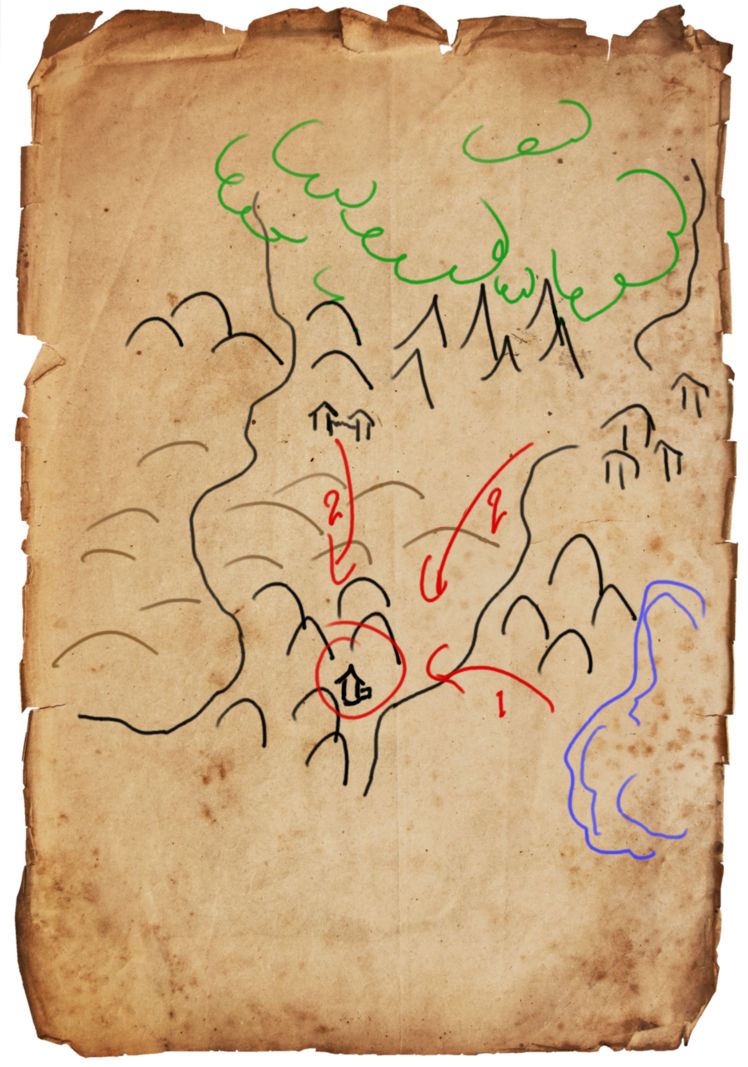
\includegraphics[width=0.9\textwidth]{fig/treasure.jpg}
  \caption*{The treasure map is old. Indicating that the ruined tower with the Torture Dungeon below lies in the Dread Duns, one day's travel west of the lake, two days' south west from Kegern, two days' south from the old keep (now only a ruin).}
\end{figure}












\clearpage
\raggedbottom
%--------|---------|---------|---------|---------|---------|---------|---------|
%       10        20        30        40        50        60        70        80
%-------------------------------------------------------------------------------
\phantomsection\addcontentsline{toc}{section}{appendix: torture dungeon}
\section*{appendix: torture dungeon}
\markboth{torture dungeon}{torture dungeon}
\label{appendixtorturedungeon}

The Old Tower and Torture Dungeon in the Dread Duns has it's own variety of undead sleeping in the laboratories and chambers below. The Undead are served by a single mad farmer, and protected on the surface by strange tower monsters.


\subsection*{mad farmer}

This old guy is just an ordinary farmer. Quite mad though. He has four dogs. Use standard stats from the core rule book.


\goodbreak 
\subsection*{tower monster}
\label{towermonster}

Large eternal guardian monsters. They attack with claws in close quarters to knock targets out of the way, and with their spike tentacles with reach up to a couple of squares away. They parry with armoured lower arms/paws. 

\

\small \begin{samepage} \begin{verbatim}
========== tower guardian =========  (size 2x2)
str 20    hp 50 abs 0
dex  7    m3 w5 r8 d12
per  8    initiative 12, ap 9
-----------------------------------
\end{verbatim} \goodbreak \begin{verbatim}
large target mod+3 to ranged attacks
claw slash 12, ap3, dam7, knockback 2
spike poke 10, ap2, dam5, pen1, reach 2 mod=0, todefend-2
bite 8, 4ap, dam10, pen2, held in maw str10, autobite each round.
arm parry 10, ap2, abs5
avoid 5, yield+2, dodge+2
mobile 2, veteran 3, balance 6, pain threshold 5
accurate 2
===================================
\end{verbatim} \end{samepage} \normalsize



\goodbreak 
\subsection*{skeleton grunt}
\label{skeletongrunt}

These undead are sorry, slow, lumbering leftovers. Sad excuses for undead. Barely intelligent and follow simple instructions. Not much magic left in them any more, after all these years.\\
They will not defend as long as they have >5hp, 3ap, M, just attack,\\
when damaged, <5hp, they will parry if attacked.

\

\small \begin{samepage} \begin{verbatim}
========== skeleton grunt =========  (skeleton02)
str  6    hp 10 abs 0
dex  5    m1 w3 r- d-
psy  3    vision 10
per  3    initiative 6, ap 4
-----------------------------------
\end{verbatim} \goodbreak \begin{verbatim}
immune to pain
no low hp mods (Black Knight 3)
takes half damage from piercing attacks
-----------------------------------
\end{verbatim} \goodbreak \begin{verbatim}
spear     5 dam 5/6, pen 1/2, abs 8, reach 1 mod-3
sword     5 dam 6, abs 10
shield    8 abs 10, parry+3
===================================
\end{verbatim} \end{samepage} \normalsize


\goodbreak 
\subsection*{skeleton guard}
\label{skeletonguard}

More powerful than their sad lost grunts. They can think independently and are evilly linked to their Master's will and intent.\\
When healthy, >5hp : 8ap, M, no parry, just attack : 2x glave\\
when damaged, <5hp, they will start defending by avoid actions.

\

\small \begin{samepage} \begin{verbatim}
========= skeleton guard ==========  (skeleton guard)
str  9    hp 15 abs 2
dex  5    m2 w4 r6 d8
psy  3    vision 15
per  9    initiative 8, 8ap
-----------------------------------
\end{verbatim} \goodbreak \begin{verbatim}
immune to pain
no low hp mods (Black Knight 3)
takes half damage from piercing attacks
-----------------------------------
\end{verbatim} \goodbreak \begin{verbatim}
glave  8 dam 9, pen 2, abs 8, parry-3, slow-1, toavoid+1
         reach 0 mod-1, reach 1 mod-0, reach 2 mod-6,
avoid  7 yield+3
===================================
\end{verbatim} \end{samepage} \normalsize


\goodbreak
\subsection*{scary skeleton Master}
\label{skeletonmaster}

The undead Master of the Tower and Torture Dungeon. All the skeleton minions are slaved to his will. He can automatically synchronise his attacks with them at no cost, and if spending an action he can effectively Oy! them into action at his initiative and synchronise them all with himself and each other across the whole dungeon. He cannot synchronise with the wraiths.

Spending an action, automatic success, he can raise/reanimate one of his fallen skeletons within range 3 at cost of 1 mana, or spending a full round he can raise/reanimate all of his fallen within range 5 at cost of 3 mana. The skeletons rise to go active next round. He can also by spending one round and 3 mana turn on the wraith generator by mental remote.

Skeletons that are manually pulled apart and dispersed, taking 1r, cannot be automatically raised/reanimated without someone spending 3r putting them back together again. They can also be smashed to pieces so they cannot be raised again by applying half full hp bludgeoning or slicing damage once they have fallen.

\

\small \begin{samepage} \begin{verbatim}
===== Undead Master Skeleton ======  (scary skeleton)
str  8    hp 20 abs 0
dex  7    m2 w4 r7 d10
int  8    vision 20
psy  8    mana 26
per  5    ap 9
-----------------------------------
\end{verbatim} \goodbreak \begin{verbatim}
immune to pain
takes half damage from piercing attacks
no low hp mods (Black Knight 3)
-----------------------------------
\end{verbatim} \goodbreak \begin{verbatim}
sword 11, duelling, poke, swing, counter attack, double 6, str bonus 2
avoid 8, yield+2
mobile 1, charge 3, rapid 5 
\end{verbatim} \goodbreak \begin{verbatim}
raise/reanimate  autosuccess, 3ap, 1 mana, range 3, one skeleton
raise/reanimate  autosuccess, 1r, 3 mana, range 5, all skeletons in range
wraith generator autosuccess, 1r, 3 mana, mental remote at any range
-----------------------------------
\end{verbatim} \goodbreak \begin{verbatim}
2x exquisite     master crafted: pen 1  abs +50%
small sword      11, dam 5(4), pen 1(0), abs 12(8), finesse-7(6)
(duelling spc)   str 2 (max +1 str bonus, max +1 str pen bonus),
                 fast+1: str 5 dex 7
                 poke: mod-1 dam-1 pen+1
                 swing: slow-1 mod-1 dam+1 todefend+1
===================================
\end{verbatim} \end{samepage} \normalsize

\

Note that the normal use of the swords are at fast+1 (2ap) speed, requiring str 5, meaning he only has one strength bonus for damage. If he use them as regular 3ap he has 2 strength bonus and gets dam+1 pen+1 for dam 5 pen 2 total.


\goodbreak 
\subsection*{wraith}
\label{wraith}

Wisps of terror and death. The fearful run away as soon as one gets close. Even the brave flee when they scream their icy shrill shriek. Close enough they will touch your heart and suck out your life. Doors or even walls cannot stop them.

\

\small \begin{samepage} \begin{verbatim}
============= wraith ==============
dex  -    hp 12 abs 0
int  4    m2 w4 r5 d6
psy  8    vision 15 night (set elf poor)
per  7    initiative 8, ap 3
-----------------------------------
\end{verbatim} \goodbreak \begin{verbatim}
can move through walls/ground
pain threshold 5
immune to non-magical physical attacks
half damage from non-magical elemental damage
full damage from magical weapons/elemental/damage
-----------------------------------
\end{verbatim} \goodbreak \begin{verbatim}
avoid 5 yield+3
touch 7 dam 1 penetrating
\end{verbatim} \end{samepage}   \   \goodbreak \begin{samepage} \begin{verbatim}
scary 3: aura 3,
    move closer (into/in aura): psy+3 vs 3
    attack melee: psy vs 3
    passing a move test gives mod+3 to future move tests
    passing an attack test gives mod+3 to future attack tests
\end{verbatim} \end{samepage}   \   \goodbreak \begin{samepage} \begin{verbatim}
touch attack: dam 1 penetrating. roll 8 vs psy on successful attack for drain,
    parried only with magical weapons, avoid is only other defence
    drains 1d4 stamina, 1d4 mana, heal self 1hp
    attacks until target passed out / dead
    magical armour protects completely: attack mod = -abs, and no penetration
\end{verbatim} \end{samepage}   \   \goodbreak \begin{samepage} \begin{verbatim}
scream attack/defence: resistance: 8 vs psy
    area range 5, psy attack to scare people away
    run away dash/run each round until not scared
    scared until passes psy roll, mod+1 cumulative per round
    Targets who recover have mod+3 against future scream attacks
    Failing a scream resistance roll resets the bonuses.
===================================
\end{verbatim} \end{samepage} \normalsize
























\clearpage
\raggedbottom
%--------|---------|---------|---------|---------|---------|---------|---------|
%       10        20        30        40        50        60        70        80
%-------------------------------------------------------------------------------
\phantomsection\addcontentsline{toc}{section}{appendix: mountain hool goblins}
\section*{appendix: mountain hool goblins}
\markboth{mountain goblins}{mountain goblins}
\label{appendixmountaingoblins}

There are two goblin clans in the BlackPeak Mountains. They have a cave each, two leagues apart, but the terrain is rugged and very slow to traverse. The two groups have very little contact and try to keep apart.

\

\todo dig out the old campaign files on nela and get the numbers, stats, and details on the hool1 clan

\


\subsection*{Blood Giant clan}

Living in the western of the two BlackPeak hools, the Blood Giant clan, scavengers and occasional opportunistic bandits and thieves. Normally they actually work for a living, menial labour in Kegern, Kleinshof, or the outlying farms when they need coin, food, or gear. The blood giants are terrified of the strange spiders of the SpiderWitch clan, and try to stay far away. Occasionally when one of them go missing they always blame the SpiderWitch, but never dare do anything about it.

In total there are about 20 heads in the Blood Giant clan. They are a sorry bunch, starved, weak, without a future. No women or runts, no loot, nothing.
XX bandits, 
XX fighters, 
XX warriors, 
XX champions, 
and the boss himself.

\

\noindent No one knows where the name comes from. What's a Blood Giant?


\subsection*{Blood Giant hool}

Sloping up from the single entrance and with very poor ventilation the hool is a death trap. Close the entrance and start a heavy smoke fire and anyone in the hool will be dead by smoke inhalation soon enough.

\


\subsection*{SpiderWitch clan}

The SpiderWitch clan lives well off of the proceeds from the wonderful spider silk cloth and clothing they produce. They can occasionally be found in the villages selling their wares and buying food, tools, and other necessities. Some of the clan members are not above stealing, but the SpiderWitch will not tolerate any behaviour which can damage their relationship with the hoomans in the area. The SpiderWitch sometimes capture lost goblins, travellers, animals, or whatnot as sacrifice to the worshipped Spider Mother.

The Witch commands six veteran fighters, eight warriors, two champions, and six archers.


\subsection*{SpiderWitch hool}

The SpiderWitch hool has a hidden escape tunnel behind the nest of the Spider Mother. The entrance slopes downwards and the cave is naturally ventilated through lots of cracks in the rock. If it rains it even has a small supply of water seeping in. 

%\
\noindent

\includegraphics[width=0.999\textwidth]{./map/hool2.png}


\goodbreak
\subsection*{Blood Giant Boss}

The chieftain, GrosOrc, is doing his limited best to keep his clan fed and alive, but that doesn't amount to much. He will accept joining forces with GamGang if persuaded at psy difficulty, or psy-3 if presented with food or women.

\

\todo finish up when access to the nela archive

\

\small \begin{samepage} \begin{verbatim}
============================================
asdfasdf
\end{verbatim} \end{samepage} \begin{samepage} \begin{verbatim}
asdfasdf
\end{verbatim} \goodbreak \begin{verbatim}
asdfasdf
\end{verbatim} \end{samepage}   \   \goodbreak \begin{samepage} \begin{verbatim}
asdfasdf
============================================
\end{verbatim} \end{samepage} \normalsize





\

\goodbreak 
\subsection*{SpiderWitch}
\label{spiderwitch}

The SpiderWitch leads her clan by the power of the Great Spider Mother. She has created a clan around herself and the massive spider monster of the cave. Apart from herself the clan is all male and functions as her own harem. She will not tolerate any female Heroes staying in her cave, psy+3 difficulty to convince, and will sneakily kill off any females when she feels able to do so. Any high charisma male Heroes are very welcome, to the point where she might choose to kidnap them if she can. Repeated application of her paralysing poison over a week or so breaks the targets mind (permanent psy-3) and bends him to her will. Roll against con, for at least three successes, one application per day.

SpiderWitch is not literate and has no grimoire to loot. She can perhaps be persuaded to teach her magic, but the spider web spell requires that the Spider Mother approves and bites the victim a few times. Say con-3 chance to survive the ordeal?

\

\small \begin{samepage} \begin{verbatim}
=========== SpiderWitch, goblin ============
str  3                    hp 11 abs 0
dex  8                    m2 w4 r6 d8
con  6                    stamina 6
int  7                    vision 20 dusk 235 goblin good
psy  8                    mana 14
per  4                    action points 5
cha  7                    xp 108
--------------------------------------------
\end{verbatim} \goodbreak \begin{verbatim}
Common 4, Svartlingo 8, haggle 5
knife 8, intercept
brawl 3, throw 2
avoid 9, yield+4, off balance
mobile 1, veteran 1, balance 9
naturally spidery, can climb perfectly, poisonous bite (see knife)
--------------------------------------------
\end{verbatim} \goodbreak \begin{verbatim}
nasty dagger  8, dam 3, pen 1, abs 6, parry-1, toparry-2, toavoid-1, finesse-7
    fast+1 (str3 dex7), good quality, evil looking, poison str 7 paralysing
    poison 7 ap-3 mp-3 until treated, roll each round for poison vs con until
    success, then the effect lasts for one day or until treated.
\end{verbatim} \end{samepage}   \   \goodbreak \begin{samepage} \begin{verbatim}
witch web  12, int 7, psy 7
    cast 1r 1m, size 3 +2/m, duration 10r +5/m
    size in sq, can be placed as caster please but contiguous
    acts as web str 8 +3/m, sticky and strong
\end{verbatim} \end{samepage}   \   \goodbreak \begin{samepage} \begin{verbatim}
force wall  8, int 3, psy 6
    cast 1r 1m, size 3 +1/m, duration 10r +5/m
    psy vs str +3/m to stop anyone passing the blocked passage
    attacks and thrown or shot objects are always blocked
\end{verbatim} \end{samepage}   \   \goodbreak \begin{samepage} \begin{verbatim}
fumbly      7, int 4, psy 4
    cast 1r 1m, duration 5r, range 5 +2/m, target 1 +1/m
    Gives a base mod-3 -1/m to all actions during the duration.
============================================
\end{verbatim} \end{samepage} \normalsize

\


\goodbreak
\subsection*{Spider Mother, the Great Queen}

A monstrously huge intelligent Spider Queen. She cooperates with the goblin clan since the SpiderWitch help feed and protect her and her brood.

The huge body is 3x3sq size, the legs are usually tucked in under the side of the body three by three, but can extend out 1sq, and the fore legs can stretch out 2sq. The fore legs are a bit larger and usually stick out 1sq forward from the body.
%\todo add image of spider token 3x3 plus placement of eight legs when tucked or stretched

Fights mainly with the two longer front legs. Stabbing with a leg can either knock back the target or hold it down for easier biting or webbing.

She can also lay web on terrain, blocking passage or ensnaring anything that enters. She can web up to 5sq/r contiguous.

\

\small \begin{samepage} \begin{verbatim}
============== Spider Mother ===============   (size 3x3) + 8x legs (small)
str 30                    hp 120 abs 2, 8x legs hp 15 abs 2
dex  7                    m4 w6 r12 d18
con 15                    vision 15 dusk 235, vibration sense
int  7                    mana 4
psy  8                    action points 6
per 14                    xp - , worth 20xp
--------------------------------------------
\end{verbatim} \goodbreak \begin{verbatim}
Common 3, Svartlingo 3, Ancient 3, spiderchitter
leg avoid 12, 2ap, (simply lifts the leg away)
body avoid 5, 4ap, yield+4 (can also lift the body so it requires reach 1 tohit)
leg stab  8, 2ap, dam 8, reach 2 mod=0, auto held down or knockback 2
    hold down str 20, mod+3 to bite or web.
bite  6, 4ap, dam 6, pen 4, poison str 8 paralysing ap-6 mp-6
web  6, 6ap, dam 2, web str 12 cumulative, no move or action except break free
double 6 (for fore legs only)
pain threshold 10, veteran 3
loosing legs: mp-1, pain+1, attacks with other than fore legs have mod-3.
\end{verbatim} \end{samepage}   \   \goodbreak \begin{samepage} \begin{verbatim}
poison str 8, ap-6 mp-6, roll each round for poison vs con until
    success, then the effect lasts for one day or until treated.

web str 12, no move or action except break free. Multiple webs are cumulative
    strength. Even broken free the target has mod-3 to all actions for each
    broken web until it's cleaned off (3r). Any weapon in contact with web gets
    a mod-3.
============================================
\end{verbatim} \end{samepage} \normalsize

\

\goodbreak 
\noindent The smaller spiderlings are nowhere near as impressive as their big momma, but still annoying in groups. They can web 1sq/r, web str 8. Their poison is str 5. They can grab with leg stabs, dragging on their target, to make it easier to bite or web.

\

\small \begin{samepage} \begin{verbatim}
================ spiderling ================   (size small)
str  3                    hp 6 abs 1
dex  8                    m3 w5 r9 d14
per  4                    initiative 14, ap 4
--------------------------------------------
\end{verbatim} \goodbreak \begin{verbatim}
spiderchitter
leg stab  7, ap 2, dam 2, double 4, auto grab-hold optional
    grab-hold str 3, target mod-3 move costs double, mod+3 to bite and web
bite  8, ap 4, dam 1, penetrating, mod-(target abs), poison str 5
web  6, ap 4, str 8, no action except break free, tohit+3, web str cumulative
avoid 7, yield+4
mobile 1, balance 6
web and poison are same as momma, but weaker
============================================
\end{verbatim} \end{samepage} \normalsize


































%\clearpage
%\raggedbottom
%%--------|---------|---------|---------|---------|---------|---------|---------|
%%       10        20        30        40        50        60        70        80
%%-------------------------------------------------------------------------------
%\phantomsection\addcontentsline{toc}{section}{appendix: monsters}
%\section*{appendix: monsters}
%\markboth{monsters}{monsters}
%%
%bla bla bla
%
%
%\subsection*{some dude}
%
%bla bla
%
%\
%
%\small \begin{samepage} \begin{verbatim}
%Some Dude
%================== human ===================
%str  4                    hp 11 abs 0
%dex  8                    m1 w4 r6 d8
%con  6                    stamina 6
%int  5                    vision 22 day 223
%psy  6                    mana 6
%per  4                    action points 3
%cha 10                    xp 108
%--------------------------------------------
%\end{verbatim} \end{samepage} \begin{samepage} \begin{verbatim}
%Common 3
%brawl 3, throw 3
%avoid 4, yield+3, off balance
%--------------------------------------------
%\end{verbatim} \goodbreak \begin{verbatim}
%money: 3 gold, 1 silver, 10 copper
%weapons
%equipment
%\end{verbatim} \end{samepage}   \   \goodbreak \begin{samepage} \begin{verbatim}
%spells
%============================================
%\end{verbatim} \end{samepage} \normalsize
%
%\
%
%\goodbreak \small \begin{samepage} \begin{verbatim}
%Other Dude
%================== human ===================
%str  4                    hp 11 abs 0
%dex  8                    m1 w4 r6 d8
%con  6                    stamina 6
%int  5                    vision 22 day 223
%psy  6                    mana 6
%per  4                    action points 3
%cha 10                    xp 108
%--------------------------------------------
%Common 3
%brawl 3, throw 3
%avoid 4, yield+3, off balance
%--------------------------------------------
%money: 3 gold, 1 silver, 10 copper
%weapons
%equipment
%\end{verbatim} \end{samepage}   \   \goodbreak \begin{samepage} \begin{verbatim}
%spells
%============================================
%\end{verbatim} \end{samepage} \normalsize
%
%\
%






















%===============================================================================
%                           P L A Y T H R O U G H
%                           ---------------------




















\clearpage
\raggedbottom
%--------|---------|---------|---------|---------|---------|---------|---------|
%       10        20        30        40        50        60        70        80
%-------------------------------------------------------------------------------
\phantomsection\addcontentsline{toc}{section}{playthrough}
\section*{playthrough}
\markboth{playthrough}{playthrough}
\label{playthrough}

\begin{readoutloud}
The idea was shitty little goblins, lots of them, tryin' and dyin'. Didn't quite turn out like I thought. Again, in my defence, some of my players can super optimise with surgical precision and managed to turn out "shitty little goblins" with the murder potential of a herd of Minotaurs led by Sauron himself.
\end{readoutloud}

\noindent The playthrough took ca 100 hours over 44 sessions. Weekday evenings with ca 2h of game time each. 
%Late 2017 to late 2019 with a seven months' gap around mid 2018. 
Most aspects worked well, some not so much. My players still said this was one of the most entertaining campaigns so far. The setting was great.

The Heroes got to almost 500xp in the end, but very little good gear. A few excellent +30-50\% abs weapons, one Hero in full plate and 2h axe, one old OP misbalanced (\texttt{dam 7/8}) legacy heavy staff. Even at the end several Heroes were fighting with damaged weapons, temporary shields, etc. \emph{That I see as success considering the tilt of this campaign.}

\begin{description}

    \item[fun:] Several aspects of the gobliny character essence lead to fun play, and my players embraced this a lot. They bicker and fight in ridiculous manner. Rarely plan ahead and even the best plans only survive a few rounds until someone has a \emph{better} plan and run off on their own on chasing whatever insane spur of the moment decision. They cheat and lie, steal money and equipment. Only one Hero had the counting skill and consistently miscounted all money and loot to privately gather quite a pile which the others never found, effectively keeping the group very poor.

    \item[slow:] Having up to six players with two goblins each, some sidekicks, and lots of ap lead to very slow rounds. This was a serious fail on my part, but is inherent to the flawed campaign design. Still, the large fights lead to interesting tactics and combat.

    \item[starving:] Having the Heroes pressed for food and money was fun. But I failed to have my human opponents flee fast enough. This gave the goblins too much food (corpses) and a little too much money and loot too early. Remember to have the opposition flee in time.

    \item[survival:] I didn't kill enough of them. They should die more often. Be brutal and establish a high death rate. Most of the opposition should be quite smart and fight well coordinated. Perhaps more humans should \emph{make certain} of kills, rendering possum less useful.

    \item[powerful:] My players are quite good at optimising characters and I underestimated how potent they could make even a bunch of goblins when they have enough of them.

    \item[SturSkurk:] I failed to get the players to attack SturSkurk early. Recommend having GammelTant threaten them with the cooking pot and Hemskelina early on so that they don't take on too many battles before trying SturSkurk at least once. It's more fun if they fail to kill SturSkurk the first time they try.
    
    \item[XP:] Since they are so many, each share of the XP from opposition and accomplishments is quite low. I rewarded all Heroes a 5xp baseline per session to establish a steady slow progression. I always enforce that all sidekicks, hirelings, and buffer bringalongs get full XP share, even the ones that died during the adventure. This limits the amount of extra bodies the Heroes will bring with them on their adventures. I also kept levelling up their sidekicks and bringalongs, as well as surviving opposition.

\end{description}

\noindent Throughout the campaign they only lost three PC Heroes and two sidekick pets. This is not nearly enough. I had expected to kill around 10 of them. They did loose almost the entire complement of GamGang bandits though, some 15+ goblins, wolves, runts. On top of that they recruited and lost another 10+ goblins and orcs. There was plenty of blood and death, just not much PC death. But they were at death's door with negative hp and precarious situations in almost every fight.

Several battles would see the Heroes loose several of their allies, with most of the Heroes themselves in serious danger, a few at or below 0hp, negative stamina and no mana left. Then manage to flee, kill off or scare away the opposition, or otherwise slink away into the night to fight another day.

\


\subsection*{Hoom Hool, where it all begins}                            % 171126

The campaign opens with four players, eight goblins and one sidekick pet. Around 90xp freshlings, highly varied builds. 

\

Session 1:\\                                                            % 171126
They get familiar with the Hoom Hool camp and cave, and with the local region map. They go through the knowledge they got from the two goblins the GamGang met and ate along the way north when fleeing the southlands. The gang has settled in at Hoom Hool over a few weeks, done one raid at Bestest Lootspot already, and scoured the woods for good eating.

Now Gamling kicks the Heroes into action and sends them off to get more food and loot. There is a small internal fisticuffs argument and the Heroes loose their first pet sidekick, a giant trained fighting rat. They quickly bring out another giant pet rat and set off towards Bestest Lootspot. The expedition is expected to take around seven days.


\subsection*{00 just another day at the office}

For opposition I brought Hjalmar Hjälte and three wagons, two carrying hireling swordsmen guards and one with an archer.
The fight was balanced to be a simple introduction. They lost one goblin and their second trained rat, several of the opposition fled the fight.

\

They started with felling a tree to block the road before the wagons show up, then spread out and hid. Waited until the wagon train arrived and two farmers got axes to chop up the tree and clear the road. Then the Heroes attacked at multiple fronts.

Hjalmar Hjälte was alone ahead of the wagons and got seriously hurt before the farmers and swordsmen could arrive to help out. He retreated, hid in a tree, and quaffed to be able to get back in the fight. The swordsmen and farmers started fighting, and the archer was harassed by a backstabbing sneaky goblin Hero(?).

\

Session 2: \\                                                           % 171203
Quickly continuing they killed one of the swordsmen before he had the time to quaff. Hjalmar Hjälte killed one goblin and a support critter. Then HH fled with the surviving archer, swordsman, and farmer. 

All carts were captured along with one donkey, the other two escaped when the goblins couldn't capture or handle them.
After re-packing the wagon and hitching the donkey they walk north out of the forest and travel back west on the grasslands but close enough to the forest to be able to flee if trouble comes for them. 

On the seventh day they arrive back at Hoom Hool, where GammelTant immediately starts cooking Victory Stew and Gamling grabs all the nice loot and cash they brought, except a few coins one of them managed to hide away in a stash in the forest close to camp.

\

Total 31 rounds, r1-9 positioning and waiting, r9-31 fight, r26-31 opposition retreat and flee. 
In the end they had killed two farmers and a swordsman. One of the Heroes was disabled and about half were hurt down below 50\% hp.


\

Loot: \\
Misc loot from the wagons and some weapons and armour from the dead humans. The corpses are mighty fine eating and they start with a few ears and fingers.
They captured all three wagons but can only take one with them since they only managed to capture one donkey. None of the goblins have ride, but one has animal handling which is enough to lead the donkey dragging the wagon. They find the hidden silver pouch in a wagon.

Awarded 10xp each for the adventure and ca 30xp to share for opposition.

\

Followup: \\
Hjalmar Hjälte survived together with a swordsman, an archer, and a farmer. They travel on to Sleepy Cove and send word to Robert the Reeve saying that the new goblin bandit gang is very dangerous and must be hunted down and killed. Hjalmar Hjälte then starts gathering a posse to hunt down the goblin bandits.

Robert moves one patrol gang to spend more time along the SouthWoods road between Sleepy Cove and Kleinshof. Thus it's more likely in the future that patrol groups are encountered in Sleepy Cove and Kleinshof, or when travelling along the road or grasslands. The patrol group won't venture into the forest alone.


\subsection*{Good Times}

With enough food to last for a while GamGang rests, relaxes, and don't do much of anything for a few days. By day 15 the larder is almost empty again and GammelTant is shouting at Gamling for more food! The next day he rounds up the Heroes and they set off to get some eating and peace of mind.

GamGang is ca 20 goblins, 10 runts, 2 wolves and minor others. They eat around 15-20 day's worth of food each day, even with part of the gang out foraging. So the wagon load of ca 100 enc simple food they looted, together with the corpses, and stretching the supply with foraging, the larder is running low in just 10 days.


\subsection*{01 robbery gone wrong}

Five players, ten goblins, the third giant rat sidekick, Gamling and one wolf. They also bring the donkey they raided last time, but no the wagon. At Bestest Lootspot they start by felling a tree and drag the trunk across the road for an ambush point, then hide, waiting for the wagon train...

The fight goes well against the wagons but when SturSkurk enters and kills Gamling the Heroes soon decide to flee:

\

% session 3                                                             % 171217
% session 4                                                             % 180107

Sessions 3-4:\\                                                 % 171217, 180107
Put up a robbery site in the NW part of the map, blocking the tight corner with a tree trunk. The wagon train enters and fighting ensues. Misc damages but no death. They cut loose a donkey to get hold of at least one wagon. The heavy wagon with the armoured-illers reach the road block and starts pushing it out of the way slowly to escape a few rounds later.

Then SturSkurk Gang arrives. The Heroes quickly notice the BigBlueBoss and his front line orcs entering the map. Gamling is closest to them, mid way between SturSkurk and rest of GamGang. Gamling charges and dies in two rounds. The others retreat and regroup. They force the farmers and archers to flee, and kill a swordsman. They loot the wagon where they cut loose the donkey, and steal the other two wagons with donkeys when they flee. Gamling is lost together with one of the Heroes. A few are at very low health and most are severely exhausted.

They manage to drag one donkey and wagon out from the fighting, laden with some random loot and the corpse of a fallen Hero. Gamling's carcass was left behind as SturSkurk Blue Boss was marching over it towards them, drenched in the blood of their fallen leader.

\

31 rounds total. r1-16 positioning and prep. r17-28 fighting wagon train. r 20-21 SturSkurk enter. r22-28 fighting both wagons and SturSkurk. r25 Gamling falls. r29-31 GamGang flees, grabbing one wagon as they go.

\

Loot:\\
They only escape with a donkey and a wagon of random loot, about 40enc simple food, a few barrels of beer, some hides, and minor coin from a dead swordsman.

Awarded 15xp each for the adventure: 10xp base, and 5xp for getting away with some loot. Then ca 24xp shared for the opposition they bested before fleeing.

\

Followup:\\
SturSkurk gang doesn't have any magical healing. Their wounds will heal at normal speed, so if the GamGang is quick to go on with \hyperref[02killthebandits]{\texttt{kill the bandits}} the opposition will still be wounded. But instead the Heroes dilly dally and delay attacking the SturSkurk camp despite GammelTant's orders.


\subsection*{Bad Times~\mdash~Death by GrimGnash}

Day 21, back at Hoom Hool. GammelTant is furious! Screaming for Revenge! The Heroes manage to get a few coins from the treasure chest for shopping some weapons in Sleepy Cove so they can attack and kill SturSkurk Blue Boss! Hemskelina has left to scout where SturSkurk can be found. She'll be back in 5-10 days if all goes well.

Sad times in GamGang Camp. Eating Fail Stew made from the goblin lost in the fight. The second cousin of a lost Hero wanders into the camp and offers his services. He's eaten a few days later since there is not enough food.

\

Next day, GammelTant gathers the whole band and tells them about the Dread Prophecy of Death by GrimGnash. When the Big Leader falls to the Blue Faced Intruder the prophecy has begun. The only way to survive is to go Kill GrimGnash before he kills them all! But no-one know who GrimGnash is, or where...


\subsection*{XX patrols} 

Four players, eight goblins. Encountering patrols on their way to Sleepy Cove to go shopping for food and weapons. Communication fails and they end up fighting the (actually quite nice) hoomans. Easy one sided fight.\\
19 rounds total, barely stopping the last soldier from escaping.

\

Session 5:\\                                                            % 180114
They pack into two wagons and head north towards the village, (day 21). Early next day, out on the grassland, they encounter a patrol. One soldier on horse and three on foot. The Horseman rides up ahead of his squad and greets them. \hyperref[misunderstandings]{Severe miscommunication ensues and the goblins attack, (page \pageref{misunderstandings}).} Contact r1-10. Fight r11-19. The soldiers are overwhelmed and they manage to kill the rider before he escapes, as well as hunt down and kill the last fleeing foot soldier, snaring him in a \emph{slow} spell.

\

Loot:\\
All the soldiers had, incl. the tasty human corpses. They manage to not kill the Horse, so now they have an good mount. The soldiers also have a small tent, a cook pot, a lamp and 100r oil, 2x flint and steel, 4x sleeping blankets, and 4 enc travel food.

Awarded 5xp each for encounter, 5xp each for victory and great style and cool timing of events in the battle, another 16xp to share for the opposition.

\

The patrol leader thought they were just some travelling traders. He tried to warn them about the goblin bandits that had been seen in the surrounding area, but the Heroes didn't understand him, all failed simple+3 Common rolls). He would also have told them that Hjalmar Hjälte was gathering a posse in Sleepy Cove to go hunt down the goblin bandits. When they got some of it they had the brilliant idea to try to push the Patrol Soldiers towards SturSkurk, telling them about the competing bandit gang. But then the goblins killed them all so no word of SturSkurk will travel back to the other lawmen.

They of course forget all about Sleepy Cove, weapons, revenge, and instead go directly back to Hoom Hool to feast on the delicious dead hoomans. GammelTant cooks Victory Stew, then aims to send them out again soon.

\

Day 23, evening. Feasted on Victory Stew, bellies stuffed round and taut. Hemskelina has not yet returned with any information on the whereabouts of SturSkurk. Did the tasty hoomans say something about a hero in Sleepy Cove? Perhaps best to go somewhere else to shop? Perhaps time to try to look for a new Hoom Hool? Somewhere further away from Sleepy Cove? The two roadkill goblins said there might be hools in the BlackPeak mountains? Wannago check it out?


\subsection*{XX mutamonsters}

The Heroes decide to go hunting for a new Hoom Hool after they fear that Hjalmar Hjälte is searching for people to form a posse to go root out the Evil Goblin menace he thinks have settled in the old Goblin Cave in the west of SouthWoods. GammelTant is against the idea since they have defeated Hjalmar Hjälte before. But seeing as Hemskelina is not yet back with the location of SturSkurk and they have enough food for a little while she doesn't care much.

Keeping to the woods so no one can find them, a couple of days later they walk through a dark and heavy section of the forest when they see small glimmering lights flit about the trees up ahead. Mmm, shiny tasty! As they approach they see large light bugs flit about, flying fish, walking lumps of moss and sticks, and a magical serene light further in the depth behind the trees. A calm relaxed feeling seeps into their minds until one of the light bugs explode and the walking moss attacks them.

Six players, 11 Heroes around 130-140xp. Approximate initial critters: 12 bugs, 4 fish, 6 lumps, 2 larva, 1 crab, spread out and not attacking in any coordinated or planned fashion. New critter entering the map in staggered spread: 8 bugs, 3 fish, 4 lumps.

Fighting 39 rounds. Three heroes almost died, two more seriously wounded. All heroes around zero stamina and no mana.
Playing the opposition mutamonster in a totally uncoordinated and simple fashion with no tactical deviousness. The players could quickly see the monstery behaviour patterns and start planning and coordinating their side of the fight.

\

% Session 6:                                                            % 180121
% Session 7:                                                            % 180128
% Session 8:                                                            % 180204
% Session 9:                                                            % 180211

Sessions 6-9:\\                                  %180121, 180128, 180204, 180211
On map they start exploring, run into exploding bugs, quickly realise the problem and change tactics. Start bolting bugs. Get stuck hammering away at moss lumps, fish and more lumps are attracted with staggered arrival. Goblins manage to control positioning and have the control of the fight until one of the larva joins in and wrecks their strategy. One goblin gets seriously wounded and has to flee the fight.

The larva gives them headaches until they can re-position their fighters for better efficiency against the heavy armoured grub and bring spear wielders to the right positions. Once they have figured out the details they immediately handle the arrival of the second larva in a quicker more efficient way, but still have problem with positioning since the heavy larva can tackle and force them out of the way easily. In the end their spell casters have near zero mana, and most fighters have very low stamina. They have also seen the big tentacle crab by now.

They kill off the second larva and the following staggered reinforcements very effectively now that they know the monster behaviour and weaknesses. They mop up the last critters, almost clearing the map, and can rest for a couple of rounds as they advance on the crab. The crab fight is relatively quick since they can bring in the heavy club wielders in the frontline, though one of them almost dies and the other gets seriously wounded.

After the crab they go for a quick cleanup to get some safe space for a bit. Then the goblins swarm the island to fiddle with the magical light while keeping occasional monsters at bay. They are surprisingly cautious and don't stay long. A few of them get mutated ability seeds, others small boosts or weird cosmetics. They also drink some of the stream waters for refreshing temporary stamina and mana reinvigoration.

\

Rounds 1-3 explore, 4-13 fight bugs, lumps, and fish.                       % s6
Rounds 14-23 mostly fighting larva, some more bugs, lumps, and fish.        % s7
Rounds 24-28 larva fight, 29-31 critter cleanup, 32-39 crab.                % s8
Rounds 39-55 cleanup and hold off for magical light fiddling.               % s9


\

Loot:\\
They bring some tasty mutamonster meat with them as they pack up. This will cause some strange issues further on. Some of them have mutated ability seeds they can choose to spend xp on later if they wish. Some got boosts and cosmetic oddities. Licking the island stone gets you weird.

\

Day 27, they have stayed near mutamonster area to rest and heal all, and now travel onward up the foothills of BlackPeak mountains, aiming for the western hool they have scouted, unbeknownst home of the Blood Giant clan.


\subsection*{XX mountain hools: BlackPeaks~\mdash~Blood Giant clan}

Finding the cave entrance they see a single lookout. They sneak up and convince him to not sound the alarm. Knife to the throat and offer of loot and women if he joins them instead of his current clan. The terrified and starving goblin happily joins GamGang, after wide eyed and wondrous questioning the quality and quantity of food, as well as women. Now they can sneak well into the cave before they are noticed.

The fight is quick, 13 rounds. With overwhelming force they kill off a couple of goblins then persuade the rest by repeating the mantra: \emph{We have Women! We have Loot!}. Blood Giant clan will be welcome into GamGang. And for GrosOrc, GammelTant is lacking a lover after Gamling died, so he will have an important job to keep her happy and cooking for them all. All in all a power grab with little bloodshed. Though one of the trigger happy Heroes kept throwing murderous black bolts long into the discussions of surrender.

\

Loot:\\
Except for the new recruits the Blood Giant clan is very poor and doesn't really have anything worth looting. A couple of days of poor food, a leaky tarp, some old rope, and a rusty dagger. The Heroes don't even bother. Even their bedding is old, mouldy, and lumpy.

\

\todo check alt version (need nela files) for notes on the hool1 attack, two sessions, search "althool1:". notes s9 says "finished in r13", without any more info. The nela campaign and note files has the full info.


\subsection*{Hoom Hool~\mdash~Feast and Fornication}

Next day they decide to travel back to Hoom Hool, introduce the newly recruited Blood Giant goblins and GrosOrc. Deliver some mutamonster meat to GammelTant as proof of the excellent location of New Hool. They also leave a heap of mutameat in a corner of New Hool. Leaving the mountains they see an IffyGriff flying out over the moors. Excellent eating! Must remember!

Back in Hoom Hool day 31 for Feast and Fornication. GammelTant is very happy with her new boytoy and the plentiful tasty meat bounty the Heroes have brought.

The next day they have discussed with GammelTant, who is still not sure about New Hool, but she agrees to bring half GamGang with her and go see for herself. The other half to remain guarding Hoom Hool.

A few days later they are back in New Hool to find that there are lots of glow fly bugs all over the place, coming from the now thoroughly rotten pile of mutameat they left behind. First order of business: pest control! 
In the end, despite all their work, GammelTant is not impressed. She does not like the indefensible properties of New Hool. She is also starting to feel a bit ill and strange. So does most of the others as well. \textit{She and everyone else has been eating a lot of mutamonster meat lately. The side effects are beginning to show}.


\subsection*{XX IffyGriff eggs}

While most of GamGang clan is being ill in New Hool the Heroes who have eaten mostly travel food is heading south into the moors to see if they can find where the IffyGriffs come from. There has been several sightings by now. The promise of wondrous super stink bird eggs for breakfast is enticing. With improved track skill they quickly find the nesting area of the IffyGriffs, an old ruined stone keep with side buildings.

But when they close in to scout the old ruins they find a camp fire burning in the ruins of the old keep. \textit{And there is a battle worn goblin warrior, barely awake, sitting lookout in a dark hidey-hole}.

\

% Session 10:                                                           % 180225
% Session 11:                                                           % 180304

Sessions 10-11:\\                                               % 180225, 180304
At night they carefully close in on the old ruin, seeing the weak light from the glowing fire pit. Their advance group manage to sneak close before the enemy lookout sees them and sounds the alarm. A small orc warband is camping in the ruins of the main keep, and does not take kindly to being snuck up on in the middle of the night.

The Heroes manage to split the enemies into two groups by lighting a large fire storm blocking the entrance arch to the ruin. This makes it easy to defeat the first wave of enemies, but leaves the main orc force behind the fire for the next wave.

The wall of fire effectively splits the warband and the Heroes quickly grind down the opposition, some of which choose to flee instead of fight a loosing battle. They even try to recruit with their previously so successful mantra: "We have Women! We have Loot!", but the orcs are not as easily impressed.

\

Rounds 1-13 fighting the first part of the warband.                        % s10
Rounds 14-20 slaughtering the first and second wave escaping the fire.     % s11
At the end three Heroes were seriously wounded, but the fight was one sided and the outcome never in doubt. The Heroes never positioned for caution or flight, just maximum kill.

\

\begin{readoutloud}
\emph{Comment in hindsight:} The warband was intended as a small but not insignificant bump. The fire wall tactic and battle map layout was \emph{very} effective to split the warband and funnel them to a kill zone. In total the warband was a varied mix of 8 orcs and 4 goblins from the standard core rules monsters chapter, including an orc champion.
\end{readoutloud}

\

Loot:\\
Dawn of day 38 sees the Heroes looting the bodies of the warband for some 14s 43c and finding a hidden stash with the warband's savings in coin and gems.

This was a high kill session and paid out 17xp each.

\

\todo finish loot section after access to nela files: d37 d38 diff, map notes

\

No IffyGriff eggs yet, but they have seen that the stink birds nest in an old tower ruin next to the ruined keep where they fought the warband.


\subsection*{New Hool illness}

\forceindent Session 12:\\                                       % 180311
They quickly travel back to New Hool to dump some loot. They are also feeling a bit off. \emph{The mutameat is not doing them any favours.} Back in New Hool everyone is ill, puking and shitting all over. Even for goblins this is a bit nasty. GammelTant blames them for the complete horror and orders all to return to Hoom Hool, but she's too sick to do anything about it. The Heroes promise her StinkBirdEggs to placate her foul mood and murderous intent. Then immediately leave New Hool to travel back to get some IffyGriff eggs.


\subsection*{IffyGriff eggs, again}

Late at night they return to the ruined keep and make camp for the night.
\emph{During the night Hjalmar Hjälte and his posse have been tracking them to the keep. Scouted the layout, and prepared to attack.}

Next day, at first dawn the goblins wake to the screams of their lookout being seriously wounded. A gang of Hoomans are attacking. They rouse in haste and manage to make a defensive stand inside the keep, limiting the damage application coming from the attackers. The fight ends quickly in just 10r. The Heroes figure out who's leading the attack and manage to blast him to pieces with concentrated fire of magic bolts in just a couple of rounds. The rest of the posse turn and flee when they see magic bombardment felling their Leader. But the Heroes they manage to capture one hired archer alive for later interrogation.

\

Rounds 1-10: wake, chaos, defence, zap-kill Hjalmar Hjälte, all the rest flee but they manage to grab one archer.

\

Later on, after looting, instead of asking the prisoner any questions one of the goblins starts torturing her, then killing her to get at the really tasty pieces before anyone else nabs them. Well, at least they have a good meal. Roasted hooman is almost as good as IffyGriff eggs.

\

Followup:\\
With Hjalmar Hjälte dead there is currently no one else mustering for posses to hunt down the goblins. Instead, the fleeing survivors have sounded the alarm at Castle Conq, and the military has dispatched Captain Burmak and a squad of his spearmen to kill off the damned goblins, now that they know they are in a poorly defensible location out on the moor.


\subsection*{Eggs, finally}

They came here for IffyGriff eggs, right? So finally they attack the nest of the monsters and after a quick fight they gather a few eggs.


\subsection*{What's in that other tower?}

There is another tower near the keep. The Heroes check it out. Finds a ghostly voice and clearly don't speak enough Ancient to have a clue about what's going on. But, Hey!, there's a great looking sword over there. Grabby grabby.

Then find out that there was something fishy about all this. The proud new owner of the magnificent old sword has difficulties letting go of the ambiance of the ruined keep. He'd rather just go back to the tower and wait there to make sure it's well guarded, in case any wrong doers are to come calling.

Troubles, troubles. Hmm. It's a nice sword, but kinda limiting. Hey! You! New Guy! Come here, we've got a great new sword for ya! And then they leave another dude to help him with the practicalities of getting food, etc.


\subsection*{New Hool~\mdash~Never Again!}

Back again with their sick comrades in the stinking New Hool. Misery! But they make everyone a great deal happier by serving stink bird eggs. They don't smell any better on the inside, but a rare delicacy for our Heroes and their kin. After food they drag everyone out of the hool, down the mountain, packed into carts, and driven, dragged, and shambled over the moors to the old keep ruin.

Fresh air and lack of mutameat is improving their health over the next couple of days. No more will they go to New Hool! GammelTant violently enforces her will that they all return to Hoom Hool!


\subsection*{Good News and Baaad News}

\forceindent Session 13:\\                                              % 180318
Day 42. Taking the fresh air out on the Moors. Frosse the fighter arrives at their ruined keep spa site, carrying news from Hemskelina. She has found where SturSkurk is camped, in the north east of SouthWoods. Great News! Revenge murder upcoming!
But worse! She has found in her travels that the hoomans are sending a military group to kill off all them bandity goblins! They call themselves Burmak and are surely soon to arrive! No time to loose!

GammelTant screams to pack up everyone and run back to Hoom Hool to stand and fight. But one of the more clever Heroes instead actually manages to persuade her that it's better if the Heroes and some fighters stay and fight the hoomans here. That way the more \emph{important} members of the clan, like GammelTant, have more time to escape back to Hoom Hool and don't run the risk of being ambushed or run down out in the open.
With that GammelTant and most of her retinue flee towards Hoom Hool, while the Heroes and a few others stay to fight.

\

Aftermath:\\
Back in Hoom Hool Goblanda gets access to some mutameat and the glow fly eggs inside. She starts tinkering to make glow fly grenades.


\subsection*{Burmak (alt version of 03 defend Hoom Hool)}

The goblins prepare for assault, and place two lookouts on alert. And whadda-ya-know, after a while the lookouts signal that a strange group of militant hoomans come marching in. The hoomans line up for a text book assault. The goblins who have already fought several fights in the area figure out how to best run defence and do their best to not die. They start a highly defensive and well positioned attrition fight.

\

Session 14:\\                                                           % YYMMDD
By attrition, well coordinated sneaky magic, and carefully timed pop out attacks they manage to inflict enough damage on the Burmak squad that several of them fall and the rest flee. Captain Burmak himself is one of the last off the map, swearing Revenge and Bloody Murder!

\

Rounds 1-27: positioning, engagement, healing, killing, lather rinse repeat.  % s13
Rounds 28-42: slow irritating murder, rest of Burmak retreat and flee.        % s14

\

Loot:\\
Excellent strategy and large kill/defeat shared xp pool pays out a huge 24xp per Hero, and some good equipment from the fallen soldiers.

\

Followup:\\
Burmak travels back to spread the word and to muster more men. But before he has the chance to get back in action the Hoomans have lost track of the Goblin Bandits. Patrols are increased, hired knights, fighters, and spellslingers are sent for to increase the military strength in the area. The Heroes run into some of them in Kleinshof later on.


% There is a long gap between session 14 and 15. Life and logistics
% 2018 april through october has no game sessions for the goblins


\subsection*{Hoom Hool~\mdash~It's Good to be Home}

\forceindent Session 15:\\                                              % 181107
All back and settled in Hoom Hool day 45. GammelTant is screaming for the head of SturSkurk. Revenge! Then they must go kill GrimGnash! And don't forget to fix food. The larder is empty and she has already cooked a runt.
The carcasses of Burmak soldiers the Heroes come home with provides a great feast and a bit of respite for the poor runts who had taken to hiding out in the woods most of the time so as not to end up swimming dead in the cook pot.

With a few days of food back home they first head off towards Kleinshof to sell of loot and get some better weapons and good food for the gang. Revenge fight is upcoming.


\subsection*{XX shopping, off to Kleinshof}

Packed up in a couple of carts with a lot of loot to sell they arrive in Kleinshof on day 50. One of the goblins have taken it upon himself to act as treasurer and loot manager for the Heroes. He's been doing an excellent job. \emph{So excellent that there seems to be no money available, ever, to buy anything. And very little loot as well. Some armour and weapons here and there, but not a lot.} The kind and accurate goblin has now trained the hoomans "Common" language to remarkably good levels to be able to properly communicate with the merchants. And trained haggle to boot.

Riding into the village they are kindly greeted by an old framer sitting on his porch, pointing the way towards the general store. Arriving, they park their carts on the market square in front of the store and go talk with the shop keeper. Showing off wares, discussing prices, haggling and gossip, they talk for a good while. The merchant calls out his nephew for a look. They whisper a bit before the young man wanders off to the inn to get a pitcher of beer for the thirsty customers.

Meanwhile the merchant winks knowingly and says he can \emph{help} with the more ... bloody ... items, for a reduced price of course. The haggling goblin has constantly failed his rolls and is glad just to get rid of the stuff and get some coin and a large amount of simple food in return. So they quickly start unloading incriminating evidence, and loading food.

\begin{readoutloud}
The merchant is no fool. He immediately sees that most of the stuff the goblins want to sell are dead men's armour and weapons, some of it clearly from Conq patrol soldiers and military groups. But he's also greedy. He will get a good price now, then help hunt down the goblins and get a reward. There is already a group of patrol soldiers resting at the Kein Kalamity inn.

But his brilliant plan has a crack. His nephew is dumb as a doorknob and totally misunderstands his instructions. The nephew goes to the inn, but immediately tells the patrol soldiers there that a group of travelling goblin tradesmen are in town and that they should come and take a look.
\end{readoutloud}

\noindent But before they can finish the nephew comes out of the Kein Kalamity inn, a pitcher of beer in hand. He has a huge grimacing smile, giggling to himself. Is that glee? Dunno, hoomans are weird.

Before they can finish loading and unloading the carts, Patrol Soldiers slowly emerge from their leisurely lunch at the Kein Kalamity inn to investigate what the local Merchant's Nephew is talking about. The lead soldier walks up to the goblins to talk and investigate, asking about their wares, plans, origin, etc. His second in command joins in. A few of the goblins slowly infiltrate the ranks as the other patrol soldiers come out of the inn.

As one of the lead goblins do a horrible job trying to explain away all the problematic items while at the same time trying to actually load the food \emph{and} drive the cart away from prying eyes the lead soldier gets irritated and tells them to stop for inspection. They argue a bit, the still moving cart trailing food packages and equipment pieces, before one of the goblins looses her patience and throws a magic black bolt at a soldier. Aaand off we go!

\

A running fight. The goblins are stretched out, trying to get the carts across the bridge and away in safety. Several of the Heroes are still mixed in with the patrol soldiers, defending and hitting back while trying to find a safe situation to disengage. A couple of the more blood thirsty goblins are still doing their best to pursue fleeing patrolmen, and didn't quite get the message that the rest are trying to disengage and get out of town with all their stuff.

\

Session 16:\\                                                           % 181114
What the Heroes didn't know was that a group of hired knights and a spellslinger was also resting at the inn, summoned to help root out some menace of the land. Being proactive they start getting ready when they hear the patrol soldiers are to go check out a strange band of travelling goblin salesmen: Didn't the summons mention goblins? Why, yes it did!

As the goblins both try to flee and fight off the patrolmen, the knights come thundering out from behind the inn, riding large war horses. Fighting patrolmen is quickly forgotten and all goblins focus on fleeing from the incoming war machines. The last cart and goblin just barely make it off map to safety. One of the Hereos stumbles off map and falls unconscious from negative hp.

\

Total of 18 rounds, strange fight, no casualties on either side.
Rounds 1-6 : flee, fight, and scatter the patrol soldiers.                 % s15
R7-18 : hunt patrol soldiers, see knights, flee and run away!              % s16
One of the Heroes almost die, just barely win initiative in the last round and stumbles off map to safety.

\

The hired knights don't pursue the goblins, opting instead to have a thorough discussion with the patrol soldiers about orders, payment, and targets. One of the patrol soldiers set off to Castle Pawa for reinforcements while the rest of the patrol group and the hirelings track down the fleeing goblins.

\

Loot:\\
The Heroes come away from their shopping with a bit of food and some silver. They still have a bit of equipment left that they never had time to unload, and they didn't have time to load all the food they bought. Some stuff also fell off the cart when they were fleeing the village.


\subsection*{02 kill the bandits}
\label{playthroughkillthebandits}

\forceindent Session 17:\\                                              % 181122
A clever idea has taken shape in the brain bumps of the smarter goblins. SturSkurk camp is not far away. They are not immediately pursued, meaning they must be tracked while the hoomans wait for reinforcements. \emph{How right they are.} So, let's lead them hoomans to SturSkurk camp and have them duke it out while the goblins wait in the shrubbery to ambush the weakened survivors.

With excellent sneak/hide rolls they lay good tracks up until they come near SturSkurk camp. There they make it look like the carts are rolled up close to the camp and disappear into it. But instead they hide the carts a bit away, expertly covering their tracks. Then they set up a great ambush and hide to await the coming hoomans. All without SturSkurk scouts finding them. Quite impressive.

\

\todo xp levels etc at s17, when got nela files

\

This turns into a highly chaotic, very large, and long fight. Raging across most of a complex 50x40sq battle map for a total of around 50 rounds. The heroes field 11 goblins, the hoomans are 12 strong, and SturSkurk with a full band of 20+ head. With sidekicks and extras there were 50+ tokens on map. \emph{Plus} all the little demons. \emph{Sooo many demons.}

It ends with five heroes hovering near death at negative hp, negative stamina, and zero mana. Another had to flee the field to survive. The rest seriously wounded. Of the hoomans only one knight and a few hirelings flee and survive, as well as Sune Summoner who took shelter in the dimensional pocket. From SturSkurk's gang only a half dozen goblins make it out alive, dragging a donkey and some treasure.

The fight spans several sessions.

\

Goblins are not good at waiting. By the time the patrol group, hired knights, and reinforcements arrive and follow the tracks to SturSkurk camp the goblins are \emph{very} antsy.

The hoomans quickly scout the escape routes from the camp, then assault. Mounted knights thundering into the camp skewering goblins and fight dogs on their lances. It takes several rounds for the SturSkurk bandits to grab weapons and start to coordinate their defence, by which time they have already lost several goblins and the hoomans have prepared an excellent battle tactic. Centre point is the hired spellslinger Sune Summoner who is opening a swirling portal, vomiting forth small lightning fast demons to swarm the camp.

\

However, at this point a couple of the Heroic but impatient Goblins have forgotten their brilliant battle plan, and screamingly charge the rear line of the hoomans' position. The battle rapidly deteriorates into a three way chaos. For a few rounds the hoomans are somewhat sandwiched between the Heroes and SturSkurk, but soon it's a very spread out free-for-all with unstructured pockets of fighting forming, flowing, and dispersing all over the place. All the while the tiny demons are streaming out of the portal attacking whatever seems interesting nearby. 

\

% s18                                                                   % 181128
% s19                                                                   % 181205
% s20                                                                   % 181212
% s21                                                                   % 181219
% s22                                                                   % 190101

Sessions 18-22:\\
The fight quickly turns to chaos. Sune Summoner is very quick to escape into the portal, leaving the demons without any guidance and direction, attacking whatever seems like a good target nearby. He also boosts the spawn rate to two demons per round for a couple of rounds before dropping it down to one per round for the next 15 rounds or so. Sune Summoner wants to make sure he has cleared the vicinity so he can climb out and escape.

SturSkurk tries to get his gang into a defensive position and drive out the knights, but it's all very chaotic and he has difficulty gathering his people. The knights meanwhile have turned around and are thundering back out to protect their support line from the vile GamGang goblins while their swordsmen isolate and slaughter as many of the SturSkurk bandits that they can.

\

After some time some of the GamGang Heroes have pushed into SturSkurk's camp and is hunting down SturSkurk Blue Boss and the Witch. SturSkurk gang is retreating and trying to escape. Several of their goblins have already started grabbing valuable loot and a donkey, preparing to escape through a bolt hole in the north east section of the palisade.

SturSkurk orcs are still trying to force the hoomans to stay outside the camp, and are pursuing retreating hired swordsmen and GamGang Heroes in total chaos. Everyone is fighting everyone else and moving around a lot.

But the hoomans are retreating. The knights have pushed off GamgGang a bit so their archers can retreat safely, guarded by their surviving swordsmen. However, on knight falls just short of escape, by focused bolts from GamGang sorcerers.

All the while everyone is trying to stem the onslaught of tiny demons that are still spilling out from the portal at an alarming rate.

\

With most of the hoomans and SturSkurk forces either dead or escaped GamGang is trying to survive, they are exhausted and many are near death. They finally kill off the last orc and swordsman and have retreated from the portal. Fewer demons come through now. GamGang can taste victory.

In the end Sune Summoner emerges from the portal and makes a dash to safety, letting the portal close a few rounds after he's gone. The few standing Heroes mop up the last few demons running loose, but cannot catch Sune.

\

Loot:\\
The Heroes slowly loot the camp and the vast field of slaughtered bodies. SturSkurk treasure is gone with the fleeing goblins but most of the camp gear is left. More than they can fit on their carts, including the SturSkurk cart and two remaining donkeys.

The hoomans have lots of good weapons and armour, and even a couple of quaffs unquaffed.

All in all they make off with quite a bit of silver and three fully laden carts with Plenty of good hooman meat. So despite the shopping going to shit, they come out on top.

There is quite a bit of xp here. 30xp from sessions, swallowing the 10xp for the adventure, 15xp for a couple of nice plans and tactics, and quite a bit of kill/defeat xp for all the opposition. I gave full xp for defeating enemies even when part of the victory was due to third party, as long as the Heroes were involved and it went according to good planning and execution.

\

Followup:\\
The surviving knight, hirelings, and patrol soldier send word for reinforcement then track the goblins back to Hoom Hool. When the message reaches Castle Conq they will dispatch Captain Lundqvist to take care of the menace once and for all.

\

\begin{readoutloud}
This was a fun battle. Tactically interesting here and there. Very much dancing on the razor's edge for the Heroes. But it was simply too large and too slow. 50-60 characters acting per round, several with multiple actions and complex behaviour. The battle took a total of 8-10h, 50r, with several rounds running over 15min each. Way too slow.

As GM I should have seen it coming and tried to force some other way. The naive plan was simply to let the Human posse and SturSkurk forces fight it out for a while in quick simplified storytelling mode until not much was left, then let the Heroes enter the fight and nicely finish it off.

But nooo. All plans are orthogonal to reality. With a couple of the Heroes simply deciding that they would rather charge the unprotected rear line of the hoomans before they had properly engaged with SturSkurk, it was just a fuckton of action all happening at once.

Fun but too slow. Try to limit the engagements. 
\end{readoutloud}


\subsection*{Hoom Hool~\mdash~Revenge Victory Stew!}

They return to Hoom Hool on day 64. The larder is empty again and GammelTant is angry but quickly turns her frown upside down to a screaming toothy grin when she is handed the corpse of SturSkurk Blue Boss himself. Revenge Victory Stew for all! She doesn't even bother to thoroughly search them for loot and treasure. Leaving them with lots of silver and plenty of food stashed away outside camp.

The evening turns into a very drunken mess when the gang finish all the beer and wine they looted from SturSkurk camp.

\

\textit{By now the knight and his group of survivors have tracked the Heroes to Hoom Hool. They lie in wait for reinforcements but decide to make an assault when the goblins are skunk drunk.}

\

Session 23:\\                                                           % 190116
The hirelings assault the camp, killing a camp babe, a couple of fighters, and wounding a few of the Heroes. The drunken Heroes fight with a drunk mod-3 mp-1 penalty, but still manage to run down and kill the knight and an archer before the rest of the hoomans flee. 

It's a quick fight, 12 rounds. Nothing remarkable. The goblins casting slow spells are murderously effective in battle, making it very difficult to defend and flee.

\

Followup:\\
The survivors will tell Lundqvist exactly how many goblins there are, how they fight, what kind of magic they use, and so on. They also set two survivors to keep track of any goblin groups leaving the camp.


\subsection*{XX shopping~\mdash~Kegern}

\begin{readoutloud}
To get smaller faster fights the players choose to bring just one goblin each, plus side kicks. So now they are a total of 6-8 characters on maps for the next adventure. The Heroes are now around 290-330xp
\end{readoutloud}

Session 24:\\                                                           % 190213
Happy and hung over, before GammelTant wakes up, they pack up a smaller shopping expedition. Just seven goblins and a sidekick. Three carts loaded with loot to sell and plenty of provisions. On the road they encounter a patrol group, but manage to talk their way out of the situation instead of just murdering them as usual. \emph{This patrol group had been away for a while and not heard about the last battles with the Heinous Goblins in the SouthWoods.}

For once the Heroes visit a village without causing a mess. They calmly enter Kegern, sell stuff, buy stuff, and place some orders with the blacksmith. They want custom work to repair a couple of damaged valuable weapons, one weapon modification, and order a couple of custom made duelling swords for a dual wielding, fast fighting goblin. The blacksmith in Kegern is happy to take the jobs, but won't be ready before day 80. So they have some time to burn. They pay about 8 gold up front, deferring the rest for later.

\begin{readoutloud}
This is a significant investment for them. They still don't have much ready cash available. Some has been taken by Gamling and GammelTant, some still locked up in loot they have not been able to sell, but a lot is also "lost" to the black hole of their accountant. I loved how that player kept the group poor, hoarding treasure, without my help. Wonderful style!
\end{readoutloud}

The old treasure map was showing something nearby in the Dread Duns, right? That's not far away from Kegern. Treasure! What can possibly go wrong?


\subsection*{XX torture dungeon}

So they leave Kegern and travel to the Dread Duns looking for whatever the map is pointing to. And with their track skill they find it pretty fast.

They cautiously approach the Tower Ruin, but don't scout properly. They see the mad farmer and his dogs. They actually try to talk with him but since he is quite off his rocker they quickly kill him and the dogs. Not scouting is an issue since now they are flanked by the two Tower Guardian monsters.

Generally easy fights, total ca 10-15r, quick damage focus with a bit of positioning. The two tower guardians have reach and lots of hp but no armour. The goblins are too many and have a couple of high damage dealers, especially against opponents without armour. So the Hereos could do a bit of dodging while the rest of the gang just flat out massacred the guardians. They did manage to position properly to limit damage application from the secondary guardian while focusing down the first one.

\

During the fights and following loot search they occasionally have to kill emerging black bugs, and soon they find where they come from. Hacking up the entrance they enter the darkness below, day 72.

\

% s25 d72 r01+                                                          % 190220
% s26 d72 r??+                                                          % 190227
% s27 d72 r49+                                                          % 190306
% s28 d72 -r81                                                          % 190410
% s29 d72 r82-r99 all exit                                              % 190605

Sessions 25-29:\\                                                       % 190220
\textit{Most of these sessions were short, finishing the dungeon took ca 7h and 99 rounds. Significant time went to discussions about tactics when fighting the wraiths and the boss group. I allowed the players to take a lot of time to discuss becuase it's an interesting tactical problem to solve, and they have a couple of clever Heroes in the group.}

\textbf{In darkness}! \emph{Yep, they forgot to bring any light}. Thankfully one of the goblins have glowing snot since the mutamonster-magic-island episode. So that's how they explore the early parts of the dungeon: he picks his nose and throws small gobs of tiny green snot-lights around. Mmm-hmm, really.

The entrance trap is an issue but they don't loose anyone to it. \textit{I had them bring an extra dude off map "to handle their donkeys", in case they would loose a Hero to the trap.}

Exploring the dungeon they slaughter black bugs and hack through slow moving skeletons. They pause here and there to look at the strange equipment, the lab cells, work tables, and have no clue what's going on.
At one point they find the wraith generator. Fiddling with it they manage to turn it on. Not good! The wraiths give them significant problems for a long time until they figure out how to burn them to death with magic fire and oil they have found.

The stasis trap exit gives them pause for a while but they manage to fiddle with it to the point where it powers up and spits out a trapped goblin adventurer. Svampinjon, the sole survivor of a team of adventurers who went to look for the treasure in the dungeon a long time ago. For Svampinjon it's been aeons in the blink of an eye. He has no clue what's going on, and the world has changed in his absence. But he pushes the idea that there must be treasure hidden somewhere, which eventually get them to search and discover the cache in the egg slime vat under the big black bug.

After much fighting and exploring they run into the undead Master of the tower. The ancient wizard, now undead thing, wakes up and start resurrecting the skeletons they have already slaughtered! So as a precaution they start spending time to completely crush and dismantle the skeletons when they can. Effective in stopping further resurrections, but time is a luxury they don't have.
And to make things worse, the undead Master also turn on the wraith generator again, and it has time to spew out several wraiths before they notice and send a fleet footed hero to turn it off again.

Exploring and fighting through the Torture Dungeon takes 99 rounds. They don't loose any Heroes, and even gain an ally. But at several times they were on the edge, with Heroes hovering around 0hp, no stamina, and running low on mana for artillery and healing. When climbing out of the dungeon most Heroes are <30\% hp and have no mana left for healing.

\

Loot:\\
They find the hidden treasure of ca 25 gold total, take a few of the ancient weapons, especially the two small duelling swords from the scary skeleton.
The freed Svampinjon, their new recruit, could also be considered as useful loot I guess.

Quite a bit of xp, 25xp for sessions swallowing the 10xp for adventure, and a bit of opposition xp per hero since they were a small group.


\subsection*{XX shopping~\mdash~Pickup in Kegern}

Arriving in Kegern day 75. They pick up their wagons from storage and go visit the blacksmith to see how he's coming along with fixing their weapons. Turns out the craftsman has been working night and day, and has already completed the work. So they pay the the man the rest of what they owe him, go out back to test their shiny arsenal, and smile happily. Before leaving the town they sell off some loot, buy food, then ride away without killing anyone at all.


\subsection*{XX mountain hools: BlackPeaks~\dash~SpiderWitch clan}

The Blood Giant goblins they recruited have talked about a second potentially good New Hool up in the BlackPeaks. The SpiderWitch clan lives there now, ruled by the SpiderWitch herself, and they are really dangerous. They eat goblins who get lost in the mountains. They ate Bob! He never came back.

Hiding the carts in the foothills and leaving a couple of guards they send a small group of Heroes up to scout the spidey-cave. In their new peaceful manner they actually approach the lookout without sneaking and simply strike up a conversation with him. Before long the Heroes are shown into the mighty fine cave and presented to the SpiderWitch herself. Feeling a bit scared by the large spiderlings crawling about, most of the Heroes stay near the entrance for a quick escape while they send in the prettiest of them all to charm her. And he does a good job. She's very pleased with the guests, proposing they stay for the night, offering to sell them some of the finest spider silk clothing.

Afraid of becoming spider food they decline the offer of lodging, but buy a shiny new hat. 
The SpiderWitch cave seems like an excellent New Hool though.


\subsection*{travelling back to Hoom Hool}

The coming days they travel homeward. Passing Kleinshof they make a wide circuit around since they think they will be recognised after their last few disasters there. Instead they send in Svampinjon, the new recruit they picked up from the Torture Dungeon. \emph{He's horrible at gossip though}. They find out that the talk of the town is that the Vile Villains have bested several posses, reinforced patrol groups, and the Burmak squad. So now Baron Conq has been forced to send Lundqvist to clear the matter once and for all! Mighty Lundqvist will vanquish and decimate any goblin bandits! A true War Hero he is!


\subsection*{XX plunder}

Taking a night's rest at the caravan camp site in SouthWoods they meet a few tradesmen who says Lundqvist will certainly kill off all of those nasty goblin bandits.

\

% s30                                                                   % 190612
% s31                                                                   % 190626

Sessions 30-31:\\
After talking with the friendly humans for a while a patrol group arrives together with the old Wagoneer, also to make night camp. Both the Wagoneer and one of the patrol soldiers recognise a couple of the Heroes from earlier fights! At least that's what the Heroes think must be happening, so they do the safe thing and strike back first.

A quick chaotic fight for 14 rounds. All but one of the patrol soldiers escape, most of the farmers, tradesmen, and hirelings as well. But they manage to kill the wagoneer, and a couple of farmers and hirelings.

Following the fight they see the strange eye-critter standing in the edge of the trees, watching. They approach and try to attack it, resulting in a chock-stun and a rapidly escaping eye-critter.

After the slaughter they of course have to flee through the night. Can't stay here and sleep! And now they are in a hurry. Everyone who escaped will scream about the Horrible Goblins.

\

Loot:\\
They have captured the mighty Wagoneer's wagon. Unfortunately the armoured-illers have escaped during the fight so they try to hitch a team of four donkeys to pull it.


\subsection*{XX posse: defeat, escape}

\forceindent Session 32:\\                                              % 190703
The escaped patrolmen and hirelings have quickly gathered reinforcements and chased down the goblins out on the plains just north of SouthWood, westward towards Hoom Hool. The Heroes are way too slow to escape with the wagon and the carts. They are attacked in the middle of the night by an unseen large force. The attacking Hoomans start seeding the Heroes general location and path with fire arrows, then rain down regular arrows on anyone who come into the light.

For 21 rounds they try to find a tactical opening but to no avail. They almost loose two Heroes without doing any serious damage to the hoomans' force. A few all-too-brave patrol soldiers flee or fall, but that's all. In the end the Heroes decide to flee and scatter into the night. A few ride away on the horse, a few escape on three donkeys, and the rest on foot. They leave the wagon, the carts, and all their loot and food behind.

\begin{readoutloud}
Since it's night and they get chased down they can't choose positioning for the fight. The never see the full human force, they just hear a lot of metal armour jingling, lots of heavy horses, and see fire arrows thumping down all around them.

The reinforced posse I brought into the darkness on map was two patrol groups, total 8 soldiers, four experienced hired archers, four experienced hired swordsmen, and two hired knights. That's two patrol groups and a medium mercenary squad. The patrol group and mercs from Sleepy Cove, and the second patrol group from the survivors and town watch.
\end{readoutloud}

%\

Loot:\\
They have to leave the wagons and just get away with what they are carrying and had stuffed in the saddle bags of the horse. They have lost all the rest of the nice loot, almost all the food, and the wagon, the carts, and two donkeys. They still have some coin left from the Torture Dungeon treasure though, as well as their nice shiny weapons.

\

Followup:\\
The posse keep tracking the goblins as best they can, back towards Hoom Hool, they also send message to sync with Lundqvist.


\subsection*{03 defend Hoom Hool: posse}

\forceindent Session 33:\\                                              % 190710
Day 80, late, after the Heroes very unheroically have fled the field and gathered back at Hoom Hool. They know the hoomans can't be far behind. They shout and scream, and run around, trying to prepare GamGang to defend Hoom Hool.

\begin{readoutloud}
The heroes are now around 350-410xp. They have just had their first large defeat and feel the pressure of the law and military bearing down on them. This is where I start wrapping up the campaign. They have played through most of the side adventures at this point, and the goblins are definitely no longer shitty little goblins, but quite powerful heroes.
\end{readoutloud}

The camp clearing, lure:\\
Outside Hoom Hool, around the cooking fire, GamGang has had a little time to prepare for an assault with a clever plan. Positioning a small group around the camp fire in the clearing to lure the hoomans to attack with confidence.
The lure will flee into the cave and trick the Hoomans force to follow them inside.

The goblins have a larger force waiting outside to attack the Hoomans in the rear, while another group is in the cave plugging up the tunnels and forcing the hoomans to clump up in the T section. This way they hope to force the hoomans into a multi-front fight in the entry way tunnels.

\

The posse arrives late in the evening. They scout the camp but fail to find the goblin assault force hidden outside. The hoomans start the assault and murder their way through the clearing and up to the opening of the cave. 

Over 22 rounds the hoomans kill a few runts and goblin fighters while "all the rest" of the bandits flee into the cave. When the hidden goblin force rush in to close the trap they manage to kill one hired archer and a few patrol soldier. One hired archer escapes and the hoomans' scouts go undetected.

\

The cave entrance, trap:\\
Closing the trap the goblin assault group kills the hooman rear guard defending the cave entrance and push into the cave. Over the first 6 rounds the strong hooman knights and experienced swordsmen slaughter eight goblin fighters and warriors. GamGang is loosing goblins too fast and the Heroes must change their tactic...

\

Session 34:\\                                                           % 190724
Switching the focus, sacrificing a couple of goblin fighters, risking a couple of the Heroes to squeeze the hoomans into the east tunnel they force the hoomans into a tight situation where they can't apply much melee strength. Aggressively throwing magic fire area spells, burning even their own people, the Heroes bottle up the hoomans enough so they in the end can pick off the front line one by one in alternate aggressive focus kills. The final eastern tunnel fight is over in only 10 rounds.

\

Aftermath:\\
The fights end with a much smaller GamGang. And they know that at least one archer fled the fight to survive. They are not safe any more. \textit{They never found the posse scouts.}

Despite their heavy recruitment and merging in most of the Blood Giant clan, after the assault GamGang is only 18 head strong, plus some runts and wolves. Morale is low. Almost all survivors are seriously wounded.

%The Heroes: 12 goblins and a sidekick giant fighting rat.
%Hemskelina, Goblanda, BoyToy(GrosOrc), one goblin fighter, one goblin warrior, one camp runt and the two mutated runts, two wolves, and three camp babes.


\subsection*{XX coup}

One of the Heroes choose this point to stage a coup. The Heroes start by healing each other as much as possible after the fight, postponing healing the gang's other fighters, GammelTant, etc. Then they send Hemskelina out with the wolves to scout the surrounding area for more hoomans, mostly to get rid of her for the coming fight.

The Heroes set the positioning of the gang so their intended New Great Leader can kill off GammelTant in a direct decisive one on one battle without much interference from the other gang members. That way they should be able to convince them of his strength, and leadership. And to increase their chances he has trained the leader skill quite high.

\

Killing GammelTant:\\
Is not as easy as one would have thought. The intended New Great Leader makes a surprise attack, but still GammelTant manages to bring him down to a 1hp before he can slay her. Almost dead he shouts to proclaim himself the new leader, to try to stop the killing of the gang members who are loyal to GammelTant. Despite their best efforts they have to kill two runts and a fighter.\\
In 5 rounds it's all over.

\

Loot:\\
They go through GammelTant's belongings and find her Crystal Ball, grimoire, and scribbled feverish notes about the Dread Prophecy of Death by GrimGnash. They also find the key to the GamGang treasure chest, not that they have much time to rejoice.

In the coming days one of the Heroes start having horrible dreams ever night about teeth and claws ripping goblins apart in varied and horrible ways. He knows that GrimGnash will kill them all! ... unless the monster can be stopped ... ?

Goblanda wants to make sure the New Leader is happy with her so she gives him a small supply of her highly unstable but quite effective new glow fly grenades.

\

\noindent All Hail Old Maz! Leader of GamGang! ... or is that MazGang?


\subsection*{03 defend Hoom Hool: proactively ambush Lundqvist}

\forceindent Session 35:\\                                              % 190731
They know the Lundqvist force is coming. Hemskelina has scouted them to be "around 12 hoomans and two horses", already only a few leagues from Hoom Hool.
\emph{Hemskelina has not seen the entire Lundqvist column. The main column is 15 strong, plus two trailing patrol soldiers on horseback. She has also missed the four sneaky outriders.}
The gang finds a good likely ambush location and set up for an attack about a league from Hoom Hool.

\

Ambush:\\
The Lundqvist force is very different from what the Heroes have fought before. They can't manage to control their positioning and focus damage like they are used to. Lundqvist is very mobile and has exceptional coordination, and the archers quickly wear down anyone who remains in line of sight and out of cover. 

The Heroes quickly loose both their wolves and a goblin champion. The Hereos reposition but soon thereafter one of the Heroes falls. All the while Lundqvist only loose one light infantry soldier and get some of his force wounded.

The Heroes quickly scatter and flee off the map, with one dead and five around 0hp. They must find some other way.

\

28 rounds for the whole ambush, ca 12r for initial positioning and waiting, and this time none of the goblins go off script and improvise when they get bored. Then a tough fight trying a few different approaches for ca 14r, then fleeing the last two rounds.


\subsection*{04 flee and relocate: to SpiderWitch hool}

\forceindent Session 36:\\                                              % 190807
They quickly send Hemskelina back to Hoom Hool to send the soft and squishy members of the gang out into the woods to hide, and the rest to form up at BlackPeak SpiderWitch hool. The main force make clear tracks as they move with haste to the SpiderWitch clan. They want to lead Lundqvist away from Hoom Hool.
\emph{Lundqvist sends a couple of scouts to track the main gang, but continues to march on Hoom Hool to root it out and burn as much as they can.}

\

The Heroes are fleeing fast and never get time to rest properly. They are running dangerously low on mana and can't heal up the survivors properly.

\

SpiderWitch:\\
Arriving at the SpiderWitch hool they are welcomed and the witch feeds them. The Heroes attempt a tall tale about having found out that Lundqvist is coming to kill SpiderWitch, and that they will help the defence. The SpiderWitch listens to them, does not figure out that they are lying, believing instead that there is a misunderstanding, and will send someone to talk with the hoomans in Kleinshof next day to sort it out. SpiderWitch has always had a good relationship with the hoomans.


\subsection*{03 Defend (temp) Hool: Lundqvist attacks SpiderWitch hool}

The SpiderWitch never gets the chance to sort things out. Lundqvist scouts have followed the Heroes and kept eyes on the SpiderWitch cave since they arrived, counting in the last few GamGang goblins arriving from Hoom Hool. All penned up and ready for slaughter.

Hemskelina has managed to track the Lundqvist main force and sneaks into SpiderWitch hool in advance to warn the Heroes. Total chaos erupts. SpiderWitch sends out a scout who doesn't return. Meanwhile the Heroes start building barricades to squeeze Lundqvist positioning and reduce their melee application, and to allow a side ambush in the darkened cave.

The Brave New Leader is indeed brave and certain of victory. He wants to kill all of Lundqvist men so none can escape to report. Again they hide an attack group close the cave entrance to attack from behind after Lundqvist force has entered.
\textit{When the Heroes send out their rear attack group of 10 goblins to hide in the cliffs and shrubs around the cave entrance, Lundqvist scout sees it.}



\textit{
Captain Lundqvist splits his force in three parts. 
The main heavy core with himself, 4 heavy, 4 light, and Dogoban the Disruptive to limit the effect of the dangerous Goblin Wizards.
The second is the support group with 4 archers, 1 light, and Sune Summoner, hired in to provide a grind down attrition option if the goblins have small cave warrens. 
Due to the scout's report he leaves a third trap group of his own, hidden outside, with 4 light and 2 archers, to plug up the cave once the Goblins trap group has entered.}

\textit{Since the Heroes don't have good enough count of the Lundqvist force they can't tell when the entire force is in the cave.}


\begin{readoutloud}
This fight is again too large and too slow. But considering that it is probably the last large fight of the campaign I choose to run with it. The cave enforces more structure, and there are only two sides this time: Lundqvist against all the goblins and spiders.
\end{readoutloud}

% s36                                                                   % 190807
% s37                                                                   % 190814
% s38                                                                   % 190828
% s39                                                                   % 190904
% s40                                                                   % 190918

Sessions 36-40, Lundqvist assault:\\
Day 83, evening. The Lundqvist force arrives, splits in the main heavy core group marching in first, the support group waiting by the entrance, and the rear trap group hiding a little bit away.

Lundqvist core march in, follow the funnel and go into heavy melee with the goblin defensive plug force. The Heroes' funnelling and surround tactics work reasonably well for a little while but Lundqvist are too focused and coordinated for the goblins to be able to put any main melee line against them and survive.

Captain lundqvist and his main core, total 10 men, slam into the goblin defense line. 

Lundqvist core heavy main heavy line enters first with Captain Lundqvist, 4 Heavy Infantry, 4 Light Infantry, and Dogoban the Disruptive. The Heroes have set up a defensive front line and a sneaky side assault, with the idea that the outside force will come in just a round or two after the last Lundqvist have entered. \textit{But Lundqvist doesn't play their game, and leaves his lighter rear force at the cave entrance for a later entry. This seriously stumps the Heroes Great Plan.}

Lundqvist main line marches straight into the goblin defense plug and start decimating it with fast synchronised attacks. Several goblins fall quickly before the side attack group can spring into action. The outside force can't enter since the Lundqvist rear guard is still formed up at the cave entrance.
The sneaky side attack group engage but is nowhere near stong enough to push the main heavy Lundqvist core into disarray. The Heroes quickly loose another skilled goblin champion and one of the strongest melee Heroes hang onto life at negative hp. Dogoban have thrown his feedback football causing serious problems for the goblin spellslinger in the side attack group.

But at least the core Lundqvist group is beset and their advance has ground to a stop. A couple of rounds later Lundqvist shout for his rear force to enter the cave.




\

\todo finish up Lundqvist hool2 fight

\

Loot:\\
They quickly loot the cave and corpses until they don't like the way the spiders are moving. Amongst the stuff is the SpiderWitch's pillow, super comfortable, giving max stamina +1 for the first fight of the day.


\begin{readoutloud}
I did not expect them to actually beat Lundqvist here. I thought they would have to flee out of the secret escape tunnel while the Spider Mother effectively covered their retreat. Then they would escape into the dark rainy mountains, bloody and beaten.

Instead now they have forced Lundqvist to retreat with a diminished force, unable to effectively pursue them. He leaves two scouts to track them, then rides north to regroup and pick up a stronger force. Next time he will \textbf{not} underestimate the devilish foe.
\end{readoutloud}


\subsection*{05 Death by GrimGnash}

\forceindent Session 41:\\                                              % 190925
The goblins flee SpiderWitch Hool. They know Lundqvist will continue to hunt them, and when the SpiderWitch died they cannot stay in the cave with the monstrous Spider Queen and her brood. They never did find out about the hidden escape tunnel, nor the SpiderWitch treasure stash. So when they leave the cave they are followed by Lundqvist scouts for a while, but later lost to the night and the rain. The Heroes disappear into the south east foothills of the BlackPeaks. Lundqvist's scouts are unable to follow.

\

Through more nightmares the New Leader has figured out that the most likely place for GrimGnash to be found is the lonely mountain top near Kegern, so he sends Hemskelina ahead to scout, while they rest for the night and heal their wounds, then begin the trek themselves the next day.

Day 85 they break camp by the high mountain. Hemskelina has returned to tell them that she has found a cave above the clouds, lit from within. She did not enter. Over the day they climb the mountain and reach the cave shortly before the sun dips towards the majestic cloud scape below them.

Determined they check their weapons and enter the cave. Ready to face GrimGnash.

\

They cautiously enter the cave, advance, and spread out to scout. It takes them a long time before they see the sleeping Dragon. Carefully sneaking up their melee force close to the Monster while their support gets into position. Then attack while the Beast still sleeps.

\

% s42                                                                   % 191002
% s43                                                                   % 191009
% s44                                                                   % 191016

\forceindent Sessions 42-44:\\   
GrimGnash immediately wakes when they attack, and with his intellect, perception, and psyche he is immediately aware of his surroundings and loose no time to force a more defensive situation by swishing his huge tail, throwing most of the close by heroes several squares further away.

\

\todo finish up GrimGnash and campaign closing

\

\begin{readoutloud}
It was a weird way to defeat GrimGnash. Suited the fun of the situation, suited the logistics of our scheduling. The evening was already quite late and I was leaving for several months. I would not have the possibility to schedule another session for quite a while. It was a good way to close the campaign.

Obviously I could have chosen to have GrimGnash be gone in the darkness for a few rounds and let the Heroes celebrate their victory. Then when they are rolling in his gold, unaware, he crawls back up out of the chasm and attacks them.

\

GrimGnash will crawl out of the underworld, eventually. Pissed and out for revenge. The GamGang / Old Maz Gang still have most of the Heroes alive, and can be used in future campaigns.
\end{readoutloud}































\clearpage
\raggedbottom
%--------|---------|---------|---------|---------|---------|---------|---------|
%       10        20        30        40        50        60        70        80
%-------------------------------------------------------------------------------
\phantomsection\addcontentsline{toc}{section}{leftovers}
\section*{leftovers}
\markboth{leftovers}{leftovers}

The idea for this campaign had been slowly crawling around in the back of my skull for quite a while when we were playing \texttt{Edwin the Chromophobe} and \texttt{Destroy the Altar}. I wanted to build a campaign for really crappy Heroes. Overdrive ridiculous. A goblin bandit gang was the obvious way to go. Lots of people have done it before, but it's still a little bit novel for most players.

Then I had a couple of years away from the game while moving around, and when I finally had the time and situation to pick up hosting the game again I had the opportunity to start with a fresh set of Heroes.

All in all, I had a good time and my players were happy with the campaign. Time well spent :)




%-------------------------------------------------------------------------------
\end{document}
